% The most entangled states of four and seven qubits.
% The paper and its supplement refer to each other: build the pair twice,
%   latexmk -pdf four_qubit_entropy.tex; latexmk -pdf supplement.tex; latexmk -g -pdf four_qubit_entropy.tex; latexmk -g -pdf supplement.tex
\documentclass[11pt]{article}
\usepackage[T1]{fontenc}
\usepackage[utf8]{inputenc}
\usepackage{lmodern}
\usepackage[a4paper,margin=23mm]{geometry}
\usepackage{amsmath,amssymb,amsthm,mathtools}
\usepackage{booktabs,longtable,array,graphicx}
\graphicspath{{figures/}}
\usepackage{xcolor,xurl}
\usepackage{xr-hyper}
\usepackage[colorlinks=true,linkcolor=blue!45!black,citecolor=blue!45!black,urlcolor=blue!45!black]{hyperref}
\newtheorem{theorem}{Theorem}
\newtheorem{lemma}[theorem]{Lemma}
\newtheorem{proposition}[theorem]{Proposition}
\newtheorem{corollary}[theorem]{Corollary}
\newtheorem{conjecture}[theorem]{Conjecture}
\theoremstyle{remark}
\newtheorem{remark}[theorem]{Remark}
\setlength{\emergencystretch}{2em}
\allowdisplaybreaks
\newcommand{\Psiico}{\Psi_{\mathrm{ico}}}
\newcommand{\Sussex}{Department of Physics \& Astronomy, University of Sussex, Brighton BN1 9QH, UK}
\newcommand{\affiliation}[1]{\\[2pt]{\small\normalfont #1}}
\newcommand{\tr}{\operatorname{tr}}
% A statement of the paper, restated in the supplement ahead of its full proof: kind, paper label, optional title.
\newenvironment{restated}[3][]{\par\addvspace{\medskipamount}\noindent\textbf{#2~\ref{#3}}%
  \ifx\relax#1\relax\else\textbf{ (#1)}\fi\textbf{.}\ \itshape}{\par\addvspace{\medskipamount}}

\externaldocument[][nocite]{supplement}
% Pointers to tables printed in the supplement.
\newcommand{\LNtab}[1]{Table~\ref{#1} of the supplement~\cite{Companion}}
\newcommand{\LNtabs}[2]{Tables~\ref{#1} and~\ref{#2} of the supplement~\cite{Companion}}
\hypersetup{pdfauthor={Antony Lewis},pdftitle={The most entangled states of four and seven qubits}}
\title{The most entangled states\\of four and seven qubits}
\author{Antony Lewis \affiliation{\Sussex}}
\date{}
\begin{document}
\maketitle
\begin{abstract}
Pure states of four and seven qubits cannot be maximally entangled across every balanced bipartition; we determine
how entangled they can be on average. For four qubits we prove the conjecture of Higuchi and Sudbery: the mean von
Neumann entropy of the three $2|2$ cuts is at most $1+\tfrac12\log_2 3$ bits, with equality exactly on the
local-unitary orbits of their state $M_4$ and its complex conjugate. For seven qubits the mean purity of the 35
balanced $3|4$ cuts is at least $121/917$ and their mean entropy is at most $2.965356029\ldots$ bits, each with a
unique optimiser up to local unitaries and qubit permutations. The two optimisers are distinct members of one
icosahedral family, so minimum purity and maximum entropy select different states.

The proofs bound moments of the marginal spectra by positive identities on several copies of the state, some of them
spin flipped, and bound the entropy by a polynomial in those moments. The four-qubit maximum has an analytic proof; the
seven-qubit proofs, and some of the four-qubit refinements below, are computer-assisted, with exact arithmetic and
rigorous error bounds. We also prove the
Gour--Wallach conjecture for R\'enyi entropies of all orders, with the maximiser changing from $M_4$ to cluster
states at $q_*\approx1.588$, and obtain sharp Tsallis bounds, mixed-state bounds and quantitative stability.

The results and text were all produced by AI agents under human supervision.
\end{abstract}

\section{Introduction}\label{sec:fqe-intro}

Multipartite entanglement requires a compromise: a state maximally entangled across one division of its qubits
need not be maximally entangled across another. A state that achieves maximal entanglement across every
bipartition is called \emph{absolutely maximally entangled} (AME). Such states are closely related to
quantum error-correcting codes~\cite{Scott} and ``perfect'' tensors~\cite{PYHP}; Ref.~\cite{AMEreview} reviews them. They exist for two, three, five and six qubits,
but not for four~\cite{HS,HSi26}, seven~\cite{HGS}, or eight or more~\cite{Scott}.
Four and seven qubits are therefore the first two sizes at which no state can maximise
entanglement across every cut simultaneously; at most four of the six two-qubit marginals, and at most 32 of the 35
three-qubit marginals, can be maximally mixed~\cite{HS,HGS,ZNSZ}. Balanced cuts expose this obstruction: if all
balanced marginals are maximally mixed, their smaller reductions are too. Conversely,
states with all one- and two-qubit marginals maximally mixed exist for every $n\ge5$~\cite{Scott},
so small marginals alone do not reveal the seven-qubit obstruction. We determine the greatest
mean entropy across balanced cuts at both sizes; minimisers of the mean balanced purity are the maximally multipartite
entangled states of Facchi et al.~\cite{FFPP}, and highly entangled states have been sought numerically since
Refs.~\cite{BSSB,Borras}. At four qubits this is the question posed by Higuchi and Sudbery in ``How entangled can two couples get?''~\cite{HS}.

Label the qubits $1,2,3,4$. There are three ways to divide them into two
groups of two:
\[
12|34,\qquad 13|24,\qquad 14|23.
\]
A \emph{bipartition}, or \emph{cut}, is balanced when its two groups are as close in size as possible:
$2|2$ here, and $3|4$ for seven qubits. For a pure state $\psi$, the reduced density matrix
$\rho_{12}=\operatorname{tr}_{34}|\psi\rangle\langle\psi|$ describes qubits $1,2$ alone; define
$\rho_{13}$ and $\rho_{14}$ similarly. Its von Neumann entropy
\[
S(\rho)=-\operatorname{tr}\rho\log_2\rho
\]
measures the entanglement across the cut. Operationally, it is the
number of Bell pairs per copy that the two sides can distil from many copies of the pure state, or need to prepare those copies,
using local operations and classical communication~\cite{BBPS}. The complementary pair has the same entropy, so each cut
is counted once. A pair of qubits
has a four-dimensional state space, so $S\le2$ bits, with equality when $\rho$ is maximally mixed,
$I_4/4$, with four equal eigenvalues $1/4$. Entropies are in bits throughout, except in the Tsallis
corollary and in proofs that use $\ln$, which say so.

We give the three cuts equal weight and study the average
\[
E(\psi)=\frac13\bigl[S(\rho_{12})+S(\rho_{13})+S(\rho_{14})\bigr]
       =\frac13\sum_{j=2}^{4}S(\rho_{1j}).
\]
It is the entanglement, in Bell pairs, available across a balanced cut chosen at random, and it is unchanged by
relabelling the qubits. Reaching $E=2$ would require all three reduced states to be
maximally mixed, hence an AME state. Their compatibility---all three come from one wavefunction---prevents
this~\cite{HS}: three maximally mixed cuts would give total purity $P=\sum_j\operatorname{tr}\rho_{1j}^2=3\cdot\tfrac14$,
whereas every pure four-qubit state has $P\ge1$ (Lemma~\ref{lem:fqe-purity}). The best average is
therefore strictly below $2$.

\paragraph{The two main results.} Higuchi and Sudbery (HS) exhibited the state
\[
M_4=\tfrac1{\sqrt6}\bigl(|0011\rangle+|1100\rangle+\omega(|0101\rangle+|1010\rangle)
+\omega^2(|0110\rangle+|1001\rangle)\bigr),\qquad\omega=e^{2\pi i/3},
\]
whose amplitudes sit on the six strings of Hamming weight two, grouped into complementary pairs, one for each
pairing of the qubits, with phases $1,\omega,\omega^2$. An even permutation of the qubits permutes the three pairings
cyclically (or fixes each of them) and only multiplies $M_4$ by a phase (Remark~\ref{rem:fqe-single-orbit}), so the three cuts are
identical: each reduced state has eigenvalues
$(\tfrac12,\tfrac16,\tfrac16,\tfrac16)$. Every cut then has the same entropy, and
$E(M_4)=1+\tfrac12\log_2 3\approx1.792$. They conjectured that this is the maximum~\cite{HS}. Brierley and Higuchi
proved that $M_4$ is a local maximum~\cite{BH}. Derksen et al.\ proved that $M_4$ maximises a different measure, the
geometric measure of entanglement (distance to the nearest product state)~\cite{DFLW}. Gour and Wallach proved the corresponding Tsallis bound among
\emph{critical} states, those whose one-qubit marginals are all maximally mixed, and conjectured the R\'enyi envelope~\cite{GW}; the precise scope of these results is at the end of this section.
Independent single-qubit unitaries are called \emph{local unitaries} (LU). Two states are \emph{LU-equivalent} if
local unitaries map one to the other up to an overall phase, and the states equivalent to a given one form its
\emph{LU orbit}. Since these operations preserve cut entropies, maximisers occur in whole LU orbits.

\medskip\noindent\emph{Theorem~\ref{thm:fqe-entropy-max} (four qubits). For every pure state of four
qubits, $E(\psi)\le1+\tfrac12\log_2 3$. Equality holds if and only if $\psi$ is equivalent to $M_4$ or
to its complex conjugate $\overline{M_4}$ by independent single-qubit unitaries.}
\medskip

At seven qubits a balanced cut puts three qubits on one side, and there are $\binom73=35$ such cuts, one for each
set $S$ of three qubits with reduced state $\rho_S$. Write
$\pi_3=\frac1{35}\sum_{|S|=3}\operatorname{tr}\rho_S^2$ and $E_3=\frac1{35}\sum_{|S|=3}S(\rho_S)$ for the mean
purity and mean entropy of the 35 cuts. An AME state
would have $\pi_3=1/8$ and $E_3=3$ bits.

\medskip\noindent\emph{Theorems~\ref{thm:fqe-seven-purity} and~\ref{thm:fqe-seven-entropy} (seven qubits). Every
pure seven-qubit state has $\pi_3\ge121/917$, with equality exactly on the local-unitary and
permutation orbit of an explicit icosahedral state $\Psiico$. Every pure seven-qubit state has
$E_3\le E_3(\psi_{x_*})=2.965356029\ldots$ bits, with equality exactly on the local-unitary and permutation orbit of
a different member $\psi_{x_*}$ of the same icosahedral family (Section~\ref{sec:fqe-seven-entropy}). With qubit labels fixed,
each equality set consists of $42$ LU orbits.}
\medskip

For four qubits, many states tie for the minimum mean purity, but the
HS cut spectra uniquely maximise the entropy. At seven qubits even the purity minimiser is globally unique (up to
local unitaries and qubit permutations), yet it is not the entropy maximiser. Both optimisers lie in one explicit
one-parameter icosahedral family, and our proofs separate them globally with five-copy certificates. ``Most entangled'' thus depends on the measure, even when only balanced cuts are compared;
at four qubits the R\'enyi entropies show the same effect, with the maximiser changing at $q_*$.

\paragraph{Four qubits: compromise between cuts.} To see why a compromise is needed, compare the four-qubit linear cluster state
$C_4=\tfrac12(|0000\rangle+|0011\rangle+|1100\rangle-|1111\rangle)$. Its entropy is $1$ bit for
$12|34$ and $2$ bits for each of the other two cuts, so $E(C_4)=5/3\approx1.667<E(M_4)$. Making two cuts
perfect costs more on the third than is gained. Figure~\ref{fig:fqe-cuts} compares the reduced-state
\emph{spectra}, or lists of eigenvalues, of the two states.

\begin{figure}[t]
\centering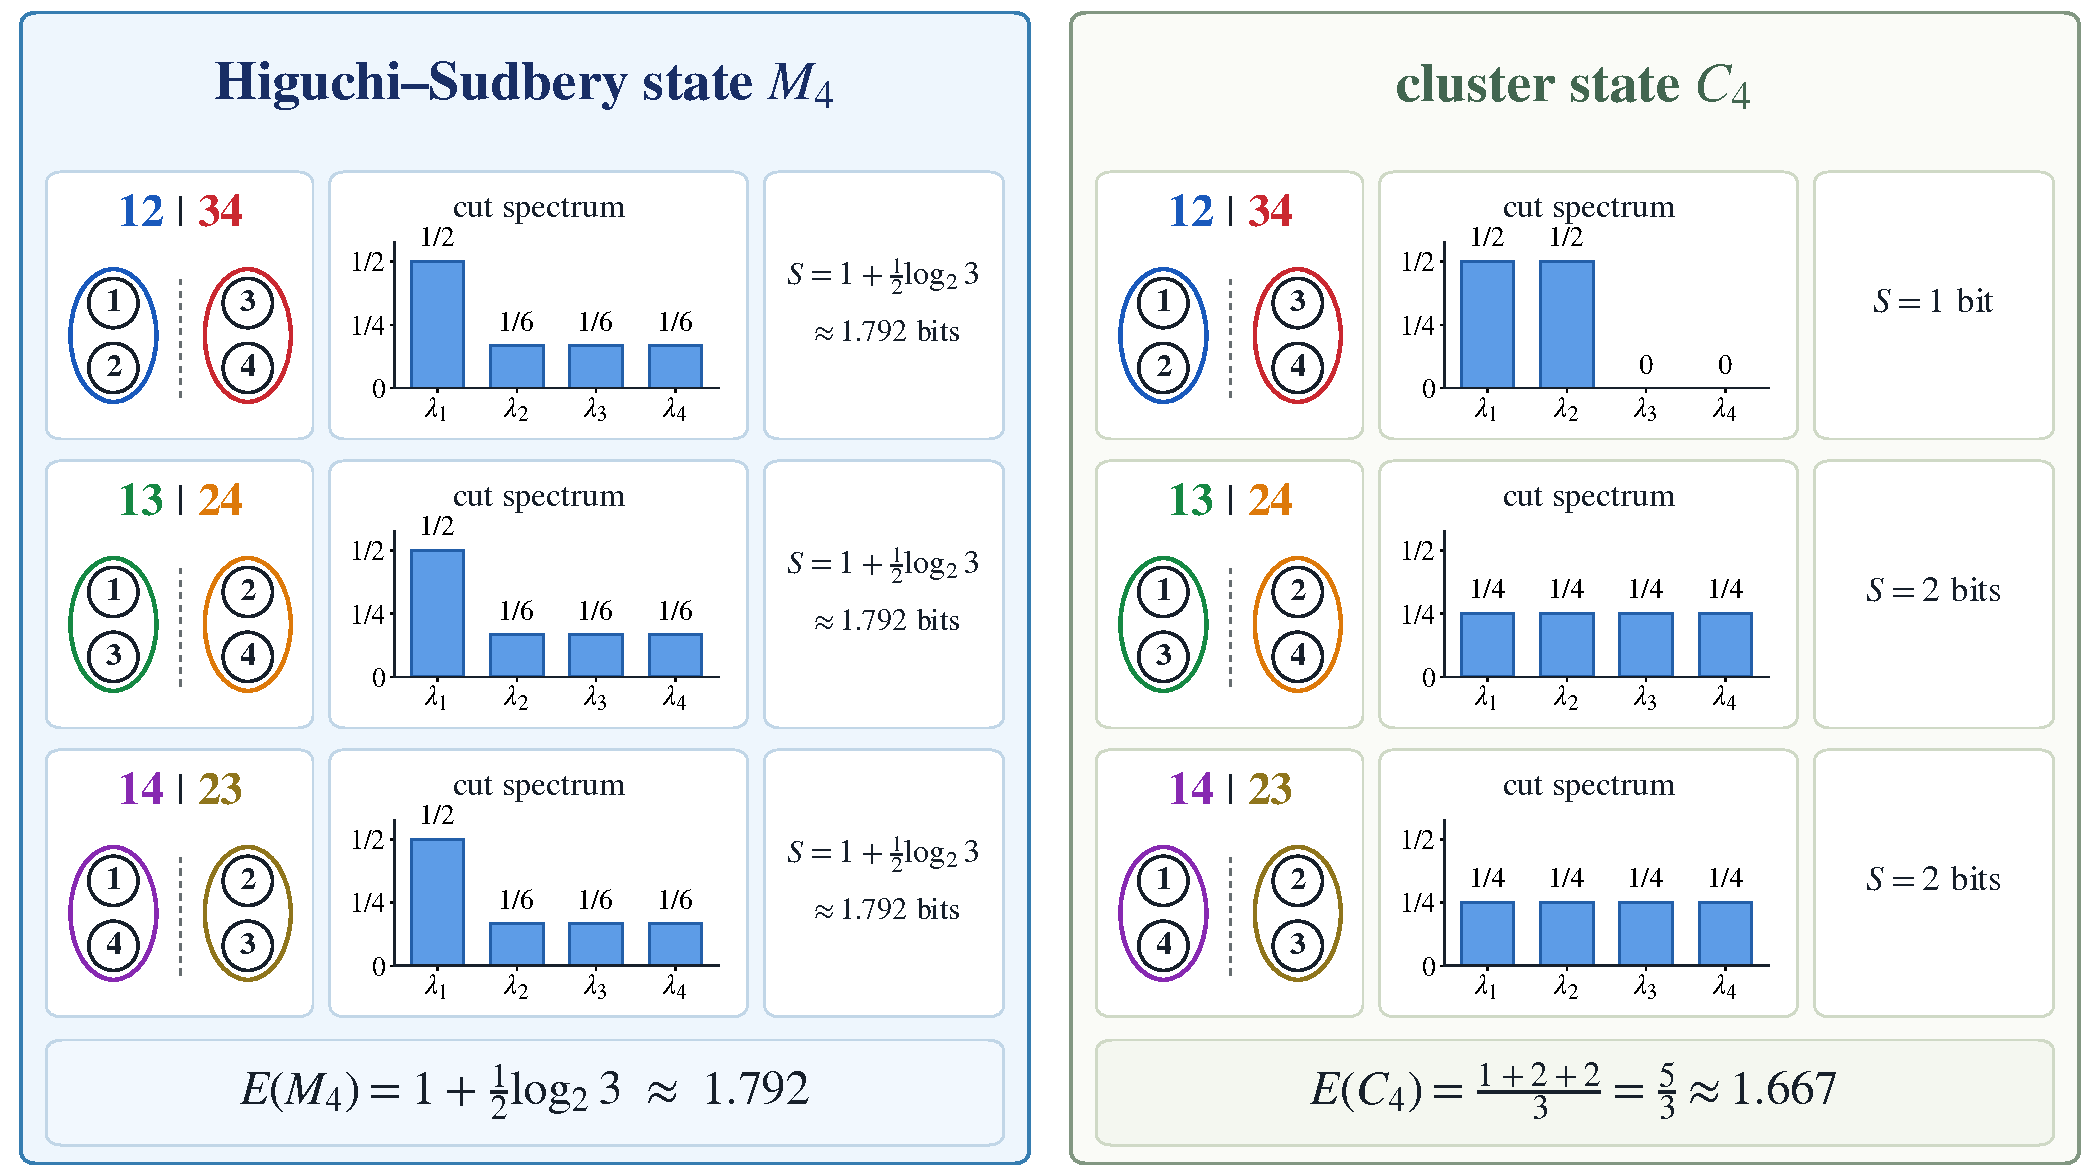
\includegraphics[width=\linewidth]{fig_cuts}
\caption{Four eigenvalues of each reduced density matrix for the three balanced
$2|2$ cuts (same vertical scale throughout). For $M_4$ each cut has spectrum
$(\tfrac12,\tfrac16,\tfrac16,\tfrac16)$ and entropy
$1+\tfrac12\log_2 3$ bits. For the cluster state $C_4$, the
$12|34$ cut has spectrum $(\tfrac12,\tfrac12,0,0)$ and entropy
$1$ bit, while the other two cuts are maximally mixed and have entropy
$2$ bits, so $E(C_4)=(1+2+2)/3=5/3<E(M_4)$: balancing the three cuts beats perfecting two at the expense of one.}
\label{fig:fqe-cuts}
\end{figure}

The LU orbits of $M_4$ and $\overline{M_4}$ are distinct~\cite[Prop.~7]{LWB} (Appendix~\ref{sec:fqe-sextic}
gives an elementary separating invariant), but an odd permutation of the qubits exchanges them
(Remark~\ref{rem:fqe-single-orbit}), so the maximiser is unique up to local unitaries and relabelling the qubits.

Purity alone cannot identify the entropy maximiser: the cluster state and $M_4$ both attain
the minimum summed purity $P=1$ but have different entropies, so a proof must also control higher moments of the cut spectra. The entanglement of
a cut depends only on the spectrum of its marginal $\rho_S$, and spectra are what copies of a state measure: $\operatorname{tr}\rho_S^k$ is the expectation value of the operator that
cyclically permutes the subsystems $S$ of $k$ copies of $\psi$. More generally, any homogeneous polynomial of degree $m$
in $|\psi\rangle\langle\psi|$ is an $m$-copy expectation value. A bound is proved by writing the gap between the bound
and the objective as the $m$-copy expectation value of a sum of manifestly positive operators $A^\dagger A$; the
optimisers are the states on which every term vanishes.

The useful positive operators also act on copies replaced by
the spin flip $\tilde\psi=\sigma_y^{\otimes n}\bar\psi$, time reversal ($\sigma_y$ composed with complex conjugation)
applied to every spin-$\tfrac12$. A Pauli string is a tensor product of Pauli matrices and identities; its weight is the number of nonidentity factors.
On density matrices, $\tilde\rho=\sigma_y^{\otimes n}\rho^T\sigma_y^{\otimes n}$ negates
the Pauli-string components of odd weight and keeps those of even weight; on one qubit it reverses the Bloch vector.
For a product state $\tilde\psi$ is orthogonal to $\psi$, while for a Bell pair it equals $\psi$ up to phase (for two qubits
$|\langle\psi|\tilde\psi\rangle|$ is Wootters' concurrence~\cite{Wootters}). Since
$\epsilon\bar u\epsilon^{-1}=u$ for $u\in SU(2)$ and $\epsilon=i\sigma_y$, a flipped copy transforms like an ordinary one, so these operators
remain local-unitary covariant.

The number of copies is set by two things. First, the entropy is not a polynomial. The proof bounds $-t\log_2t$ by a
\emph{majorant}, a polynomial lying above it on $[0,1]$, that touches it at the optimiser's eigenvalues,
and the degree needed grows with the number of touching points (Section~\ref{sec:fqe-entropy_maximum-entropy-bound}). The cuts of $M_4$ have spectrum
$(\tfrac12,\tfrac16,\tfrac16,\tfrac16)$, with two distinct eigenvalues, so a cubic suffices: two copies give $P\ge1$ and
three bound the cubic moments. Second, a few copies may not be enough even for a polynomial objective. Allowing
$m=2,3,\dots$ copies gives a \emph{hierarchy} of ever stronger bounds, but a few copies constrain only low-order
correlations between copies, and they admit moment data that pass every positivity test at that level yet come from no pure state.
At seven qubits both the purity and the entropy need five copies; Section~\ref{sec:fqe-seven-entropy} explains why and
compares the two sizes in Table~\ref{tab:fqe-four-seven}.

\paragraph{The four-qubit proof.} Write $P$ and $T$ for the sums of the second and third
moments of the three two-qubit marginals, and $F=17P-12T-12$. The two-copy spin flip~\cite{GW,WC} gives $P\ge1$
(Lemma~\ref{lem:fqe-purity}); a three-copy sum of squared tensor norms, the sextic identity, gives
$F\ge0$, that is $T\le5/12+(17/12)(P-1)$ (Theorem~\ref{thm:fqe-moment} and Appendix~\ref{sec:fqe-sextic}).
A cubic majorant of $-x\ln x$, its Hermite interpolant (the cubic matching its value and slope at $1/6$ and $1/2$,
which lies above it), turns these
moment bounds into the entropy bound. With $\Delta_H\ge0$ the total gap of the majorant over the twelve cut eigenvalues,
the entropy gap is
\[
3\ln2\,\bigl[E(M_4)-E(\psi)\bigr]=\bigl(\tfrac{15}{2}-6\ln3\bigr)(P-1)+\tfrac32(\ln3-1)F+\Delta_H,
\]
with all three terms nonnegative (Section~\ref{sec:fqe-entropy_maximum-entropy-bound},
equation~\eqref{eq:fqe-entropy-gap}). Equality forces $P=1$ and every cut eigenvalue to be $1/6$ or $1/2$, hence the $M_4$ spectrum
on each cut; the critical normal form identifies the state from just one cut
(Proposition~\ref{prop:fqe-onecut}). The classification of all zeros of the
moment inequality, also given in Appendix~\ref{sec:fqe-sextic}, is not needed for equality.

\paragraph{Relation to earlier work.} Gour and Wallach studied the analogous optimisation for Tsallis and R\'enyi
entropies~\cite{GW}, including a conjecture on R\'enyi entropies that we prove (Corollary~\ref{cor:fqe-renyi-gw}).\footnote{It is distinct from the statement on four-qubit states maximising the absolute value of the
hyperdeterminant that is usually called the Gour--Wallach conjecture, proved by Chen and
\DJ{}okovi\'c~\cite{CD}.} Their Theorem~10(a) proves the Tsallis-entropy bound for exponents $0<q<2$
among the critical states (the normal form of~\cite{VDD}), with the
bound attained by $M_4$. It does not cover every pure state. Their equality clause names only the class of $M_4$;
with labelled qubits $M_4$ and its conjugate are distinct LU classes, exchanged by an odd permutation
(Remark~\ref{rem:fqe-single-orbit}). For $q>2$ their Theorem~9(a) identifies the unrestricted Tsallis maximiser, a
state other than $M_4$ (we prove only that the cluster state beats $M_4$ there), and their Theorem~12 identifies the cluster-state maximisers of the
R\'enyi entropies for $q\ge2$~\cite{GW}; Corollary~\ref{cor:fqe-renyi-two-up} gives a self-contained
elementary proof of that high-order ceiling and its equality cut spectra. For the von Neumann entropy itself, this paper supplies
a short, self-contained analytic proof of the bound for all pure states, the classification of the
equality case, and unrestricted corollaries for other spectral entropies.\footnote{A proof of the unrestricted entropy bound and its attainment at $M_4$, with a Lean verification, appeared
independently while this work was in preparation~\cite{Omega}; it does not address uniqueness of the maximiser or the
equality case, and we make no priority claim for the moment inequality as such.}
At seven qubits, earlier numerical searches found mean three-qubit purities of $0.13387$~\cite{Facchi}
and $0.131952$~\cite{DMFF18}; the latter agrees with our minimum $121/917$ to six digits. \emph{Stabilizer states},
joint eigenstates of $n$ commuting, independent Pauli strings (graph states and the cluster state $C_4$ are examples), do worse: the best,
including that of Zha et al., have purity $19/140\approx0.1357$~\cite{Zha11,HGS}.
Before this work, the best explicit universal lower bound known to us was the
unattainable AME value $1/8$; Rico et al.\ obtained a numerical semidefinite
estimate of $0.127(8)$~\cite{Rico}, without a certificate. It agrees with the exact three-copy bound
$\pi_3\ge125/978\approx0.12781$ proved here (Table~\ref{tab:fqe-seven-levels}), the three-copy level of our hierarchy.

\paragraph{Proofs and verification.} The four-qubit von Neumann bound and its
equality case have a fully analytic proof here. Some extensions, particularly at
seven qubits, use exact-rational or rigorously bounded numerical certificates.
Table~\ref{tab:fqe-guide} is a roadmap of the paper: for each result it gives the optimiser, how it is proved
and where the complete proof is. The supplement uses S-prefixed numbering; the companion
repository~\cite{Companion} contains both documents, the scripts and their
captured outputs, and the Lean formalisation. Appendix~\ref{sec:fqe-verifiers} lists the computer checks
behind each result, and \texttt{verifiers/MAP.md} maps them to scripts. The analytic arguments do not depend on Lean.
Every theorem, proposition, lemma and corollary is proved, analytically or with the exact and computer-assisted checks named in its proof; numerical observations are labelled as such. Table~\ref{tab:fqe-other-n} in Section~\ref{sec:fqe-discussion} collects what is known at other qubit counts.

\begin{table}[htbp]
\centering\small
\begin{tabular}{@{}p{0.19\linewidth}p{0.17\linewidth}p{0.33\linewidth}p{0.23\linewidth}@{}}
\toprule
Question & Optimiser & How proved & Where \\
\midrule
Four qubits: maximum mean entropy & $M_4$, $\overline{M_4}$ &
Analytic (two- and three-copy identities, cubic majorant) &
Sections~\ref{sec:fqe-entropy_maximum-purity-identity}--\ref{sec:fqe-entropy_maximum-equality-and-one-cut-rigidity};
Appendices~\ref{sec:fqe-sextic}, \ref{sec:fqe-normal-form} \\\addlinespace
Four qubits: Tsallis $0<q<2$ & $M_4$ & Analytic (same majorant) &
Section~\ref{sec:fqe-spectral}; Appendix~\ref{sec:fqe-spectral-proofs} \\\addlinespace
Four qubits: R\'enyi $0<q<1$ & $M_4$ & Analytic (from the Tsallis bound) &
Section~\ref{sec:fqe-spectral} \\\addlinespace
Four qubits: R\'enyi $1<q<2$ & $M_4$ for $q<q_*$, cluster for $q>q_*$ &
Analytic with exact finite checks &
Appendix~\ref{sec:fqe-renyi-proofs}; supplement, Section~\ref{sec:sup-renyi} \\\addlinespace
Four qubits: R\'enyi $q\ge2$ & cluster & Analytic (elementary purity bound) &
Appendix~\ref{sec:fqe-renyi-high-order} \\\addlinespace
Four qubits: orbit stability & -- & Analytic with exact finite checks; some constants computer-assisted with rigorous error bounds &
Section~\ref{sec:fqe-stability-summary}; Appendix~\ref{sec:fqe-orbit-stability}; supplement, Sections~\ref{sec:fqe-stability-proofs}, \ref{sec:sup-stability} \\\addlinespace
Seven qubits: minimum mean purity & $\Psiico$ & Computer-assisted with rigorous error bounds (five-copy identity) &
Appendices~\ref{sec:fqe-seven}, \ref{sec:ico}; supplement, Section~\ref{sec:fivecopy} \\\addlinespace
Seven qubits: maximum mean entropy & $\psi_{x_*}\ne\Psiico$ & Computer-assisted with rigorous error bounds (five-copy identity, joint majorant) &
Supplement, Section~\ref{sec:sup-seven-entropy}; uses Theorem~\ref{thm:fqe-seven-purity} \\
\bottomrule
\end{tabular}
\caption{Optimisers, methods and the location of complete proofs. Optimisers are listed up to local unitaries and qubit
permutations; both classes attain the R\'enyi bound at $q=q_*$. Supplementary sections have an S prefix. Exact finite checks use exact arithmetic; computer-assisted
proofs evaluate explicit identities in floating point with rigorous error bounds. Neither uses a numerical search as
evidence. Appendix~\ref{sec:fqe-verifiers} lists the checks behind each result.}
\label{tab:fqe-guide}\label{tab:fqe-proof-guide}
\end{table}

\section{The four-qubit maximum}\label{sec:fqe-main}

Throughout this section, $\psi$ is a unit four-qubit state, $E(\psi)=\frac13\sum_{j=2}^4S(\rho_{1j})$ is its average
$2|2$ entropy in bits, and $M_4$ is the Higuchi--Sudbery state, all as defined in
Section~\ref{sec:fqe-intro}. Write the one-qubit marginals as
$\rho_i=(I+\mathbf r_i\cdot\boldsymbol\sigma)/2$, where $\boldsymbol\sigma$ is the vector of Pauli matrices
and $\mathbf r_i$ is the Bloch vector.

\begin{theorem}[maximum and equality]\label{thm:fqe-entropy-max} For every unit $\psi\in(\mathbb
C^2)^{\otimes4}$,
\[
E(\psi)\le 1+\tfrac12\log_2 3 ,
\]
with equality if and only if $\psi$ is local-unitarily equivalent to $M_4$ or to $\overline{M_4}$.
\end{theorem}

The bound is proved in Sections~\ref{sec:fqe-entropy_maximum-purity-identity}--\ref{sec:fqe-entropy_maximum-entropy-bound}
and the equality case in Section~\ref{sec:fqe-entropy_maximum-equality-and-one-cut-rigidity}; the two
orbits are related by a qubit permutation in Remark~\ref{rem:fqe-single-orbit}.

\begin{table}[htbp]
\centering\small
\begin{tabular}{@{}ll@{}}
\toprule
Symbol (unit states) & Meaning \\
\midrule
$P=\sum_{j=2}^4\operatorname{tr}\rho_{1j}^2$ & Sum of the cut purities \\
$T=\sum_{j=2}^4\operatorname{tr}\rho_{1j}^3$ & Sum of the third moments \\
$F=17P-12T-12$ & Nonnegative defect in the third-moment bound \\
$W_1=\sum_{i=1}^4\|\mathbf r_i\|^2$ & Total squared one-qubit Bloch-vector length \\
$\tau=|\psi^T\sigma_y^{\otimes4}\psi|^2$ & Squared spin-flip overlap (four-tangle) \\
\bottomrule
\end{tabular}
\caption{Notation for the four-qubit proof. A state is critical when all $\mathbf r_i=0$, equivalently
when all one-qubit marginals are maximally mixed. Homogeneous formulas below use $N=\|z\|^2$
and unnormalised marginals; unit states have $N=1$.}
\label{tab:fqe-moment-notation}
\end{table}

\subsection{Purity identity}\label{sec:fqe-entropy_maximum-purity-identity}

The first ingredient bounds the sum of the three cut purities. Its equality condition also
identifies the locus on which an entropy maximiser must lie.

\begin{lemma}[purity identity]\label{lem:fqe-purity} For a unit state, $P=\sum_{j=2}^4\operatorname{tr}\rho_{1j}^2=1+\tfrac12\Delta$ with
$\Delta=\sum_{i=1}^4\|\mathbf r_i\|^2+\tau$, where $\mathbf r_i$ are the one-qubit Bloch
vectors and $\tau=|\psi^T\sigma_y^{\otimes4}\psi|^2$. In particular $P\ge 1$, with equality iff all
$\mathbf r_i=0$ (critical) and $\tau=0$.

\end{lemma}

\noindent Here $\tau$ is the four-tangle of Wong and Christensen~\cite{WC}, and the lemma is
Gour and Wallach's identity $\tau_2=(4\tau_1-\tau_{ABCD})/3$~\cite[Theorem~6]{GW}, with
$\tau_k$ the averaged linear entropies $2(1-\operatorname{tr}\rho^2)$ of the $k$-qubit
marginals. We include the short spin-flip proof to keep the argument self-contained.

\begin{proof} For a \(2\times2\) matrix \(A\), spin flip is \(\sigma_y
A^T\sigma_y=(\operatorname{tr}A)I-A\). Tensoring this identity over the four qubits, a product
operator \(A_1\otimes\cdots\otimes A_4\) is sent to \(\bigotimes_i\bigl((\operatorname{tr}A_i)I-A_i\bigr)\).
By linearity the spin flip \(\tilde\rho=\sigma_y^{\otimes4}\rho^T\sigma_y^{\otimes4}\) of a four-qubit
density matrix is
\(\tilde\rho=\sum_{S\subseteq\{1,\ldots,4\}}(-1)^{|S|}\rho_S\otimes I_{S^c}\), where \(\rho_S\) is the
marginal on the sites in \(S\) and \(\rho_\varnothing=1\). Since
\(\operatorname{tr}[\rho(\rho_S\otimes I)]=\operatorname{tr}\rho_S^2\), \[
\operatorname{tr}(\rho\tilde\rho)=\sum_{S}(-1)^{|S|}\operatorname{tr}\rho_S^2 .
\] For \(\rho=|\psi\rangle\langle\psi|\) we have \(\rho^T=|\bar\psi\rangle\langle\bar\psi|\), hence
\(\tilde\rho=|\tilde\psi\rangle\langle\tilde\psi|\) with \(\tilde\psi=\sigma_y^{\otimes4}\bar\psi\), and
\[
\operatorname{tr}(\rho\tilde\rho)=|\langle\psi|\tilde\psi\rangle|^2
=|\psi^\dagger\sigma_y^{\otimes4}\bar\psi|^2=|\psi^T\sigma_y^{\otimes4}\psi|^2=\tau ,
\] because \(\psi^\dagger\sigma_y^{\otimes4}\bar\psi\) is the complex conjugate of
\(\psi^T\sigma_y^{\otimes4}\psi\) (as \((\sigma_y^{\otimes4})^*=\sigma_y^{\otimes4}\)). For a pure
four-qubit state, complementary purities agree (\(\operatorname{tr}\rho_S^2=\operatorname{tr}\rho_{S^c}^2\)),
so the sum has the two terms \(S=\varnothing,\{1,2,3,4\}\) equal to \(1\), the eight terms with
\(|S|=1,3\) adding to \(-2\sum_i\operatorname{tr}\rho_i^2\), and the six terms with \(|S|=2\)
adding to \(2P\): \(\tau=2-2\sum_i\operatorname{tr}\rho_i^2+2P\). Now
\(\operatorname{tr}\rho_i^2=(1+\|\mathbf r_i\|^2)/2\) gives the result. \end{proof}

\noindent Every term of $P-1=\tfrac12\Delta$ is quadratic in $|\psi\rangle\langle\psi|$ and hence an expectation value in two copies
of the state. The term $\tau$ is the squared overlap of one copy with the spin flip of the other. This two-copy positivity is the first
level of the hierarchy used at seven qubits (defined in Section~\ref{sec:fqe-seven-entropy} and
Appendix~\ref{sec:fqe-seven}).

\subsection{The sharp moment inequality}\label{sec:fqe-entropy_maximum-the-sharp-moment-inequality}

The purity bound alone does not give the sharp entropy bound. We also need to constrain the third
moments of the same marginals. We state this bound homogeneously so that its sum-of-squares identity
applies to unnormalised vectors.

For \(z\in\mathbb C^{16}\), write \(N=\|z\|^2\) and let \(R_{1j}\) be its unnormalised reduced matrix
on qubits \(1,j\). Put \[
P=\sum_{j=2}^4\operatorname{tr}R_{1j}^2,\qquad
T=\sum_{j=2}^4\operatorname{tr}R_{1j}^3,\qquad
F=17NP-12T-12N^3.
\]
For unnormalised \(z\) the letters \(P,T\) denote these homogeneous moments; at \(N=1\) they reduce to the unit-state
\(P,T\) of Table~\ref{tab:fqe-moment-notation}, and \(F=17P-12T-12\).

\begin{theorem}[moment inequality with polarisation remainder]\label{thm:fqe-moment} Let
$W_1=\sum_i\sum_{a=x,y,z}\langle z|\sigma_a^{(i)}|z\rangle^2$. Then
\[
F(z)\ge\frac34NW_1\ge0,
\]
and the constant $3/4$ is attained by every product state.
For unit states this implies $T\le5/12+(17/12)(P-1)$. The state $M_4$ has $(P,T)=(1,5/12)$ and a
product of two Bell pairs has $(3/2,9/8)$; both satisfy $F=0$, so both lie on the line
$T=5/12+(17/12)(P-1)$. Consequently $17/12$ is the least $\kappa$ for which
$T\le5/12+\kappa(P-1)$ holds for all unit states (the Bell point forces $\kappa\ge17/12$).
Every zero $z\ne0$ of $F$ is critical: all its one-qubit marginals are $NI/2$.

\end{theorem}

\begin{proof} The key identity expresses the moment defect as a sum of three kinds of nonnegative terms: one-qubit
polarisation, the squared norms of contractions of two copies of the state with one spin-flipped copy, and the
disagreement between the actions of the one-qubit marginals on the state. Let \(\epsilon=i\sigma_y\), \(\tilde z=\epsilon^{\otimes4}\bar z=\sigma_y^{\otimes4}\bar z\) and
\(w=z\otimes z\otimes\tilde z\), so that each qubit carries three slots \(x,y,t\), one from each copy. At one qubit define
maps from three slots to one by \(L|xyt\rangle=\epsilon_{yt}|x\rangle\) and \(M|xyt\rangle=\epsilon_{xt}|y\rangle\). Let
\(S_i\) be the orthogonal projector onto the symmetric subspace of the three slots of qubit \(i\), and contract the other
three qubits:
\[
U_i=S_i\!\prod_{j\ne i}L_jw,\qquad V_i=S_i\!\prod_{j\ne i}(L_j+M_j)w,
\]
vectors on six qubits. Write \(R_i\) for the unnormalised one-qubit marginal of \(z\) and \(R_i^{(i)}\) for its action on
qubit \(i\) of \(\mathbb C^{16}\). Appendix~\ref{sec:fqe-sextic} proves the identity \[
\boxed{\quad8F=6NW_1+3\sum_i\|V_i-8U_i\|^2+12\sum_{i<j}\bigl\|(R_i^{(i)}-R_j^{(j)})z\bigr\|^2.\quad}
\tag{S}\label{eq:fqe-remainder}
\] Identity~\eqref{eq:fqe-remainder} is a polynomial identity of degree six in the amplitudes of $z$, that is, cubic in
$|z\rangle\langle z|$ (a three-copy identity); we call it the \emph{sextic identity}.
The derivation uses contractions with the two-dimensional antisymmetric tensor, the vanishing of three-vector
antisymmetrisation in dimension two, and elementary swap traces. Nonnegativity and criticality follow at once. At a
product state of norm \(N\) every \(R_i^{(i)}z=Nz\) and \(F=3N^3=\tfrac34NW_1\). \end{proof}

\subsection{Entropy bound}\label{sec:fqe-entropy_maximum-entropy-bound}

We now combine the two moment bounds with a scalar interpolation inequality.
The resulting gap formula makes both the bound and its equality conditions explicit.

Let \(f(x)=-x\ln x\), and let \(h\) be its cubic Hermite interpolant at the nodes \(\xi_1=\tfrac16\) and
\(\xi_2=\tfrac12\): it agrees with \(f\) and \(f'\) at both nodes. Its cubic and quadratic coefficients
are \[
a=18(\ln3-1)>0,\qquad b=18-\tfrac{39}2\ln3 .
\] These coefficients are fixed by matching \(f\) and \(f'\) at both nodes.
Since \(f^{(4)}(x)=-2/x^3<0\), the Hermite remainder has the sign
\[
h(x)-f(x)=-\frac{f^{(4)}(\zeta_x)}{4!}
       (x-\tfrac16)^2(x-\tfrac12)^2\ge0\qquad(x>0),
\]
for some \(\zeta_x>0\). Equality occurs only at the two nodes; at the
endpoint \(x=0\), \(h(0)-f(0)=\tfrac12-\tfrac38\ln3>0\).
Thus \(h\) majorises the entropy function on the entire spectral interval
(Figure~\ref{fig:fqe-majorant}). In general a polynomial majorant of $-t\log_2t$ on $[0,1]$ touching it at $k$
interior points has degree at least $2k-1$, attained by the Hermite interpolant
(Proposition~\ref{prop:seven-entropy-majorant-degree} of the supplement). Two tangencies thus need a cubic; at seven
qubits this degree count leads to a two-variable majorant (Section~\ref{sec:fqe-seven-entropy}).

\begin{figure}[t]
\centering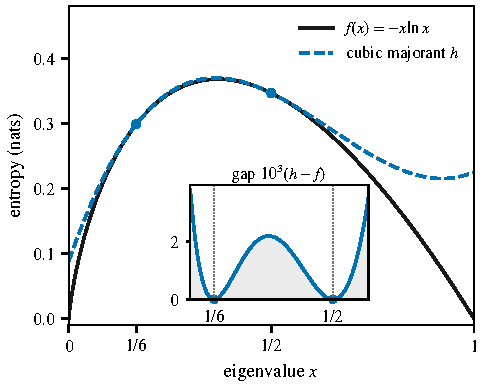
\includegraphics[width=0.5\linewidth]{fig_majorant}
\caption{The single-eigenvalue entropy contribution $f(x)=-x\ln x$ (in nats) and its cubic majorant $h$, tangent at the eigenvalues $1/6$ and $1/2$
of every cut of $M_4$. The inset magnifies the gap $h-f$ by $10^3$ on $[0.1,0.6]$: it is nonnegative, with double zeros at the nodes.
Summing $h$ over the cut spectra gives an affine upper bound on the entropy in terms of $P$ and $T$;
equality in this scalar bound requires every eigenvalue to be at a node.}
\label{fig:fqe-majorant}
\end{figure}

Return now to unit states. Each cut has four eigenvalues \(\lambda\) with \(\sum\lambda=1\),
\(\sum\lambda^2=\mathrm{tr}\rho_{1j}^2\), \(\sum\lambda^3=\mathrm{tr}\rho_{1j}^3\). Summing \(h\) over the 12
eigenvalues of the three cuts, \[
3\ln2\;E(\psi)=\sum_{j,\lambda}f(\lambda)=\kappa_0+bP+aT-\Delta_H,\qquad
\Delta_H=\sum_{j,\lambda}(h-f)(\lambda)\ge0,
\] with a constant \(\kappa_0\) independent of \(\psi\). At \(M_4\) every cut has spectrum
\((\tfrac12,\tfrac16,\tfrac16,\tfrac16)\), so \(\Delta_H=0\), \(P=1\), \(T=\tfrac5{12}\) and
\(E(M_4)=\tfrac12+\tfrac12\log_26=1+\tfrac12\log_23\). Subtracting, and using \(T=(17P-12-F)/12\)
(the definition of \(F\) at \(N=1\)), \[
\begin{aligned}
3\ln2\,\bigl(E(M_4)-E(\psi)\bigr)
&=-b(P-1)-a\bigl(T-\tfrac5{12}\bigr)+\Delta_H\\
&=\bigl(\tfrac{15}{2}-6\ln3\bigr)(P-1)
+\tfrac32(\ln3-1)F+\Delta_H.
\end{aligned}\tag{EG}\label{eq:fqe-entropy-gap}
\] Here \(-b-\tfrac{17}{12}a=\tfrac{15}2-6\ln3\) and \(a/12=\tfrac32(\ln3-1)\). All three terms
are nonnegative: \(\tfrac{15}2-6\ln3>0\) (since \(1<\ln3<5/4\)), \(P\ge1\)
(Lemma~\ref{lem:fqe-purity}), \(F\ge0\) (Theorem~\ref{thm:fqe-moment}), \(\Delta_H\ge0\). This
proves \(E(\psi)\le E(M_4)=1+\tfrac12\log_23\).

\paragraph{Why the bound is tight.} The entropy bound uses only the nonnegativity of $F$, rather than its stronger polarisation remainder. Its unit zeros are exactly the two
$M_4$ LU orbits and the three LU orbits of products of two Bell pairs, one for each pairing of the qubits
(Proposition~\ref{prop:fqe-moment-zeros} of Appendix~\ref{sec:fqe-sextic}). Only the two HS orbits saturate the entropy bound,
since products of two Bell pairs have $P=\tfrac32$. The cubic majorant touches the entropy function exactly at the eigenvalues of $M_4$, and
its coefficient signs make both moment slacks, $P-1$ and $F$, enter~\eqref{eq:fqe-entropy-gap} with nonnegative
weights. The same criterion yields the Tsallis bound for $0<q<2$ and the R\'enyi bound for $0<q<1$
(Proposition~\ref{prop:fqe-majorant}). At Tsallis order $q=2$ all critical states with $\tau=0$ tie.
Appendix~\ref{sec:fqe-correlation} gives a correlation-volume interpretation of the moment inequality. The sextic identity also
controls the spin flip: for unit states $F\ge\frac34W_1+\tau-\tau^{3/2}$ (Theorem~\ref{thm:fqe-general-envelope}), with equality on
product states and, for every $\tau\in[0,1]$, on a family of critical states. With the gap formula~\eqref{eq:fqe-entropy-gap}
this gives the Tsallis and von Neumann stability estimates in $W_1$ and $\tau$ of Appendix~\ref{sec:fqe-spectral-proofs}.

Being cubic in $|\psi\rangle\langle\psi|$, the sextic identity is a certificate at the three-copy level of the same
hierarchy, for the objective $F$ instead of a purity (Appendix~\ref{sec:fqe-seven}).

\subsection{Equality and one-cut rigidity}\label{sec:fqe-entropy_maximum-equality-and-one-cut-rigidity}

\begin{proposition}[one-cut rigidity]\label{prop:fqe-onecut} If $P=1$ and a $2|2$ cut has spectrum
$(1/2,1/6,1/6,1/6)$, then $\psi$ is LU-equivalent to $M_4$ or $\overline{M_4}$.

\end{proposition}

\begin{proof} Relabel the chosen cut as \(12|34\). Lemma~\ref{lem:fqe-purity} gives criticality and
\(\tau=0\). Write two-qubit states in the Bell basis with the phases of the magic basis,
\[
m_1=\tfrac1{\sqrt2}(|00\rangle+|11\rangle),\quad
m_2=\tfrac{i}{\sqrt2}(|01\rangle+|10\rangle),\quad
m_3=\tfrac1{\sqrt2}(|01\rangle-|10\rangle),\quad
m_4=\tfrac{i}{\sqrt2}(|00\rangle-|11\rangle),
\]
and a four-qubit state as \(\psi=\sum_{j,k}Z_{jk}\,m_j\otimes m_k\), with qubits \(1,2\) indexing the rows of \(Z\) and
qubits \(3,4\) the columns. In this basis single-qubit unitaries on each pair act, up to phase, as real four-dimensional rotations, so
local unitaries act by \(Z\mapsto O_1ZO_2^T\) with \(O_1,O_2\in SO(4)\). By the critical normal form
(Theorem~\ref{thm:fqe-critical-normal-form} of Appendix~\ref{sec:fqe-normal-form}), \(\psi\) is LU-equivalent to \(G(v)=\sum_kv_k\,m_k\otimes m_k\), that is
\(Z=\operatorname{diag}(v)\), with \(v\in\mathbb C^4\) a unit vector. The
cut spectrum and \(\tau\) are LU invariant (the latter by
\eqref{eq:fqe-spin-flip-normal-form}). On \(G(v)\) the spectrum of the cut \(12|34\) is
\(\{|v_k|^2\}\) (the \(m_k\) are orthonormal), and \(\tau=|\sum_kv_k^2|^2\) by
\eqref{eq:fqe-spin-flip-normal-form}.
Fix the large coordinate to \(1/\sqrt2\) by a common phase. Then \(\tau=0\) says that the other three
squares have modulus \(1/6\) and sum to \(-1/2\). Their sum has the largest possible modulus,
\(3(1/6)=1/2\), so equality in the triangle inequality forces all three squares to equal \(-1/6\). Thus, up to position of the large coordinate,
\[
 v=(\sqrt3,\pm i,\pm i,\pm i)/\sqrt6.
\]
The rotations \(Z\mapsto O_1ZO_2^T\) reduce these sign choices to two.
Applying the same determinant-one signed permutation on both sides of $G(v)$
moves the large entry to the first position without changing the other entries
except for their order. A diagonal rotation on one side can flip any pair of
small signs. Thus only their parity matters, giving the representatives
$(\sqrt3,i,i,i)/\sqrt6$ and $(\sqrt3,-i,-i,-i)/\sqrt6$.
Expanding the $m_k$ shows that
\[
 M_4=G\bigl((1,1,i\sqrt3,1)/\sqrt6\bigr).
\]
Multiplying by $-i$ and moving its third coordinate to the first gives the second representative.
Complex conjugation gives the first, since each $m_k\otimes m_k$ is a real vector, so $\overline{G(v)}=G(\bar v)$. Both representatives therefore belong to the stated pair
of LU orbits.
Relabelling preserves the pair of orbits, since it permutes the coefficient triple
\((1,\omega,\omega^2)\) up to common phase and conjugation.
\end{proof}

\emph{Proof of equality in Theorem~\ref{thm:fqe-entropy-max}.} Suppose $E(\psi)=E(M_4)$. The
positive coefficients in \eqref{eq:fqe-entropy-gap} force $P=1$ and $\Delta_H=0$.
The strict Hermite remainder above then forces every cut eigenvalue to be
$\tfrac16$ or $\tfrac12$. Four such eigenvalues with sum $1$ are
$(\tfrac12,\tfrac16,\tfrac16,\tfrac16)$, so Proposition~\ref{prop:fqe-onecut} applied to any one cut
shows that $\psi$ is LU-equivalent to $M_4$ or $\overline{M_4}$. This identifies the equality states without classifying all zeros
of $F$ or separately excluding Bell-pair products. Conversely, $M_4$ and its conjugate
have this spectrum on every cut and attain the bound. This proves Theorem~\ref{thm:fqe-entropy-max},
including equality.

\begin{remark}[a single orbit]\label{rem:fqe-single-orbit} The transposition of qubits $2$ and $3$
exchanges $|0011\rangle\leftrightarrow|0101\rangle$ and $|1100\rangle\leftrightarrow|1010\rangle$ and
fixes $|0110\rangle$ and $|1001\rangle$. It therefore sends the coefficient triple
$(1,\omega,\omega^2)$ of $M_4$ to $(\omega,1,\omega^2)=\omega\,(1,\omega^2,\omega)$, that is,
\[
M_4\longmapsto\omega\,\overline{M_4}.
\]
Since $E$ is invariant under qubit
permutations and $\omega$ is a global phase, the two local-unitary orbits of
Theorem~\ref{thm:fqe-entropy-max} are exchanged by a permutation of the qubits: the set of maximisers
is a single orbit under local unitaries together with qubit permutations. This is a special case of
the observation of Lyons, Arnold and Swogger~\cite{LAS}: even permutations of the qubits fix $M_4$ up to
phase, and odd ones map it to $\overline{M_4}$.
\end{remark}


\section{R\'enyi, Tsallis and mixed-state entropies}\label{sec:fqe-spectral}

Different spectral entropies give different weights to the marginal eigenvalues. For $q>0$, $q\ne1$, the R\'enyi~\cite{Renyi} and Tsallis~\cite{Tsallis} entropies
\[
 H_q(\rho)=\frac{\log_2\operatorname{tr}\rho^q}{1-q},\qquad
 S_q(\rho)=\frac{1-\operatorname{tr}\rho^q}{q-1}
\]
tend as $q\to1$ to $S(\rho)$ in bits and $(\ln2)S(\rho)$ in nats,
respectively. As $q\to0$, $H_q$ tends to the base-two logarithm of the rank of $\rho$, which is the Schmidt rank across a pure-state cut; $H_2=-\log_2\operatorname{tr}\rho^2$ is fixed by the
purity, the quantity minimised at seven qubits and the one that randomised-measurement experiments estimate
directly~\cite{Brydges19}; as $q\to\infty$, $H_q$ depends only on the largest eigenvalue. Each is Schur-concave: averaging any pair of eigenvalues cannot lower it. For
pure states it therefore does not increase under deterministic local operations and classical communication~\cite{Nielsen99}:
every member measures how entangled a cut is. Asking which state maximises them all tests whether ``most entangled''
is a robust notion. The answer depends on the order: $M_4$ maximises the mean R\'enyi entropy for $q<q_*\approx1.588$, and the cluster states maximise it for $q>q_*$. For the Tsallis entropies $M_4$ is the maximiser for $0<q<2$; the cluster states tie with it at $q=2$ and beat it for every $q>2$. The
maximiser for $q>2$ is identified by Gour and Wallach~\cite[Theorem~9(a)]{GW}; we do not reprove that result. The cut spectra explain the change. Those of the cluster state are
flat, $(\tfrac12,\tfrac12)$ on one cut and uniform $\tfrac14$ on the other two, so its mean R\'enyi entropy is $5/3$ for
every $q$; the lopsided spectrum $(\tfrac12,\tfrac16,\tfrac16,\tfrac16)$ of $M_4$ gives a mean $H_q$ falling from
$2$ bits as $q\to0$ to $1$ bit as $q\to\infty$. Small $q$ favours full rank and large $q$ a small largest
eigenvalue, hence the crossing at $q_*$. The Tsallis tie at $q=2$ holds because $1-\operatorname{tr}\rho^2$ depends
only on the cut purities, and both states have $P=1$.

The cubic-majorant argument applies to a wider class of spectral functionals. We state that criterion and
apply it to Tsallis entropies and R\'enyi orders below one; orders above one need additional estimates
(Appendix~\ref{sec:fqe-renyi-proofs}). We then transfer the pure-state bounds to mixed-state convex roofs. We retain
the notation \(P,T,F,\tau\) from the maximum proof; proofs not given here are in Appendix~\ref{sec:fqe-spectral-proofs}.

\begin{proposition}[Cubic spectral majorants]\label{prop:fqe-majorant}
For continuous $f:[0,1]\to\mathbb R$, set
\[
\mathcal E_f(\psi)=\frac13\sum_{j=2}^4\operatorname{tr}f(\rho_{1j}).
\]
Suppose $h(x)=ax^3+bx^2+cx+d$ majorises $f$ on $[0,1]$, agrees with $f$
at $1/6$ and $1/2$, and satisfies $a\ge0$, $b+17a/12\le0$.
Then $\mathcal E_f(\psi)\le\mathcal E_f(M_4)$ for every pure four-qubit state.
If both coefficient inequalities are strict, equality holds precisely on the two HS LU orbits.
\end{proposition}
\begin{proof}
Put $\alpha=-b-17a/12$ and
$\Delta_f=\sum_{j,\lambda\in\operatorname{spec}\rho_{1j}}(h-f)(\lambda)\ge0$.
Summing the cubic and subtracting its value at $M_4$ gives
\[
3\bigl(\mathcal E_f(M_4)-\mathcal E_f(\psi)\bigr)
=\alpha(P-1)+\frac a{12}F+\Delta_f.\tag{SF}\label{eq:fqe-spectral}
\]
All three terms are nonnegative, since $P\ge1$ (Lemma~\ref{lem:fqe-purity}) and $F\ge0$
(Theorem~\ref{thm:fqe-moment}). The same two nonnegative moment defects therefore control every functional
satisfying the coefficient conditions. If $a,\alpha>0$, equality requires $P=1$ and $F=0$,
so Proposition~\ref{prop:fqe-moment-zeros} gives the HS orbits; the other zeros of $F$, the products of two Bell pairs,
have $P=3/2$ and are excluded. No strict scalar
majorisation is required. For differentiable $f$, a candidate touching cubic
is its Hermite interpolant at the two nodes.
\end{proof}

\begin{corollary}[Tsallis entropies]\label{cor:fqe-tsallis} For every \(0<q<2\), \(q\ne1\), the mean
Tsallis-\(q\) entropy of the three cuts satisfies \[
\boxed{\quad
\tfrac13\sum_{j=2}^4\frac{1-\operatorname{tr}\rho_{1j}^q}{q-1}
\ \le\ \frac{1-2^{-q}-3\,6^{-q}}{q-1}\quad}
\] with equality iff \(\psi\) is LU-equivalent to \(M_4\) or \(\overline{M_4}\). \end{corollary}
The range is sharp: at \(q=2\) equality is no longer unique, and for every \(q>2\) the cluster state beats \(M_4\)
(proved in Appendix~\ref{sec:fqe-spectral-proofs}, which also gives the corresponding quadratic deficit bounds).

\paragraph{R\'enyi entropies.} With $H_q$ as above, write
\[
\mathcal E_q(\psi)=\frac13\sum_{j=2}^4H_q(\rho_{1j}),\qquad
h_q=\mathcal E_q(M_4)=\frac{\log_2(2^{-q}+3\,6^{-q})}{1-q}.
\]
At $q=1$ these have their continuous von Neumann values in bits.

\begin{corollary}[R\'enyi entropies below one]\label{cor:fqe-renyi} For \(0<q<1\), concavity of
\(\log\) and the Tsallis bound imply \[
\frac13\sum_{j=2}^4
\frac{\log_2\operatorname{tr}\rho_{1j}^q}{1-q}
\le \frac{\log_2(2^{-q}+3\,6^{-q})}{1-q},
\] again with exactly the same LU equality classes. The argument does not assert the analogous R\'enyi
bound for \(q>1\).

\end{corollary}
\noindent Equality needs equality in the Tsallis bound, hence the HS orbits, and in Jensen's inequality for the logarithm
over the three cuts, which holds there because the three cuts of $M_4$ have identical spectra.

Orders above one require additional estimates. The full result is as follows, with $q_*$ the
unique order for which $h_{q_*}=5/3$ (Proposition~\ref{prop:fqe-renyi-crossing}).

\begin{corollary}[R\'enyi envelope of Gour and Wallach]\label{cor:fqe-renyi-gw}
For every pure four-qubit state and every $q>0$, $\mathcal E_q(\psi)\le\max\{h_q,5/3\}$.
For $q<q_*$ the maximisers are exactly the two HS LU orbits;
for $q>q_*$ they are the cluster states up to local unitaries and qubit permutations (every permutation of the three cuts is induced by a permutation of the qubits).
At $q=q_*$ both classes, and only those classes, attain the bound.
\end{corollary}
Below one the bound follows from the preceding corollary, and at $q=1$ from
Theorem~\ref{thm:fqe-entropy-max}. For $q>1$ it is proved in Appendix~\ref{sec:fqe-renyi-proofs}, which opens with a
plan of the argument; for $1<q<2$ the proof is analytic apart from exact finite checks, namely an exact six-copy
certificate bounding the variance of the three cut purities and exact polynomial sign checks.
Figure~\ref{fig:fqe-renyi} shows the change of maximiser.

\begin{figure}[t]
\centering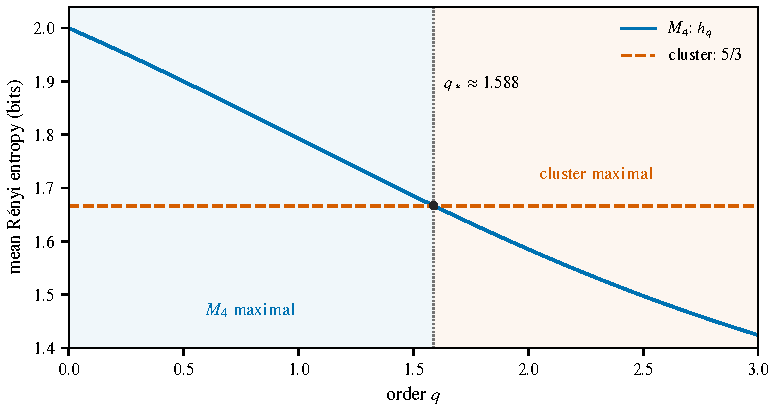
\includegraphics[width=0.8\linewidth]{fig_renyi}
\caption{Change of R\'enyi-entropy maximiser with the order $q$. The mean entropy of $M_4$
($h_q$, solid) and that of the cluster states ($5/3$, dashed) cross once, at $q_*\approx1.588$
(Proposition~\ref{prop:fqe-renyi-crossing}). The larger of the two, $\max\{h_q,5/3\}$,
is the maximum over all pure four-qubit states (Corollary~\ref{cor:fqe-renyi-gw}):
$M_4$ attains it below $q_*$ and the cluster states above $q_*$ (shaded regions). Values at $q=0$ and $q=1$
are continuous limits.}
\label{fig:fqe-renyi}
\end{figure}

\subsection{Mixed-state entanglement}\label{sec:fqe-spectral_corollaries-mixed-state-entanglement}

For a mixed state, the entropy of a marginal also counts classical mixing, which is not entanglement: the
maximally mixed four-qubit state has maximally mixed marginals but no entanglement. We therefore use the
\emph{convex roof}: the least average of a pure-state spectral functional over all ensembles representing the state,
as in the entanglement of formation~\cite{BDSW}.
For a general $f$ obeying the hypotheses below, this construction is an entanglement
monotone when the induced function of the marginal is concave and vanishes on pure marginals, as for the von
Neumann and Tsallis entropies; the ceiling below needs neither property.
In the cut notation below, $\widehat{1j}$ denotes the complementary pair.

\begin{corollary}[Convex roofs]\label{cor:fqe-convex-roof} Let \(f\) satisfy the hypotheses of
Proposition~\ref{prop:fqe-majorant}. For each cut define the convex roof \[
E_f^{1j|\widehat{1j}}(\rho)=
\inf_{\rho=\sum_\ell p_\ell|\psi_\ell\rangle\langle\psi_\ell|}
\sum_\ell p_\ell\operatorname{tr}f(\rho_{1j}^{(\ell)}).
\] Then every mixed four-qubit state satisfies \[
\frac13\sum_{j=2}^4 E_f^{1j|\widehat{1j}}(\rho)
\le\mathcal E_f(M_4).
\] If both coefficient inequalities of Proposition~\ref{prop:fqe-majorant} are strict, equality holds exactly
for pure states in the two \(M_4\) LU orbits. For \(f=-x\log_2x\) these are the three bipartite
entanglements of formation. The same HS ceiling and pure-only equality classification hold for
the Tsallis entropies with $0<q<2$ and the R\'enyi entropies with $0<q<q_*$, including their
von Neumann limits at $q=1$.

\end{corollary}
To prove the ceiling, fix any pure-state ensemble $\rho=\sum_\ell p_\ell|\psi_\ell\rangle\langle\psi_\ell|$.
Each cut's roof is at most that cut's ensemble average, so the mean of the three roofs is at most
$\sum_\ell p_\ell\,\mathcal E_f(\psi_\ell)\le\mathcal E_f(M_4)$ by Proposition~\ref{prop:fqe-majorant} (in the R\'enyi case, with
$\mathcal E_q$ in place of $\mathcal E_f$, by Corollary~\ref{cor:fqe-renyi-gw}). Appendix~\ref{sec:fqe-spectral-proofs} excludes mixed maximisers:
every mixed-state support contains a vector of deficient Schmidt rank (fewer than four nonzero Schmidt coefficients
across a given $2|2$ cut), whereas every pure maximiser has full rank there.


\section{Stability of the four-qubit maximum}\label{sec:fqe-stability-summary}
A nearly maximal four-qubit entropy forces the state close to a maximising orbit. Let $d(\psi)$ be the minimum Hilbert-space
distance from a unit state $\psi$ to the LU orbits of $M_4$ and $\overline{M_4}$, allowing a global phase, and
$\delta(\psi)=1+\frac12\log_23-E(\psi)$ the entropy deficit. Then $\delta\ge d^2/20$ for every pure state
(Theorem~\ref{thm:fqe-orbit-stability}): an entropy within $\varepsilon$ of the maximum guarantees distance at most
$\sqrt{20\varepsilon}$ from a maximiser. Near the orbits the bound improves to $\delta\ge\frac3{10}d^2$ when $d\le1/20$,
and the power two is optimal. On the critical locus, where all one-qubit marginals are maximally mixed, the optimal
bound is $\delta\ge C_*d^2$ with $C_*\approx0.19058$, attained by explicit states (Theorem~\ref{thm:fqe-p1-sharp}),
so no universal coefficient can exceed $C_*$. The coefficient
$\tfrac3{10}$ holds only for $d\le1/20$, whereas the states attaining $C_*$ lie at distance $d\approx0.55$. The proof compares the infidelity to the orbits with a sextic moment
defect, with optimal coefficient one (Theorem~\ref{thm:fqe-global-overlap}). The same estimates transfer
to the Tsallis entropies of Section~\ref{sec:fqe-spectral} (Corollary~\ref{cor:fqe-orbit-spectral}).
Appendix~\ref{sec:fqe-orbit-stability} states these results with their constants and proof strategy.

\section{Seven qubits: compatible moments and entropy}\label{sec:fqe-seven-entropy}

The four-qubit proof bounds compatible marginal moments and then converts those bounds into an entropy bound.
We follow the same strategy for seven qubits, where AME states again do not exist~\cite{HGS}.
Five-copy positivity determines the purity minimum and its equality orbit. For entropy, a majorant involving
each marginal and its spin flip gives a second five-copy certificate. The two optima occur at different
members of one icosahedral family.

\paragraph{The two optimisation problems.} A balanced cut divides the seven qubits into groups of three and four.
It suffices to consider the three-qubit side $S$, whose reduced state $\rho_S$ has eight eigenvalues. There are
$\binom73=35$ such subsets, and we average over all of them:
\[
 E_3(\psi)=\frac1{35}\sum_{|S|=3}S(\rho_S),\qquad
 \pi_3(\psi)=\frac1{35}\sum_{|S|=3}\operatorname{tr}\rho_S^2 .
\]
Every cut has entropy at most $3$ bits and purity at least $1/8$, and reaching either bound on every cut
would require an AME state.

The mean purity has a direct interpretation in terms of correlations. Expanding each marginal in Pauli strings writes $\pi_3$ as $1/8$ plus a
positively weighted sum of the squared expectation values of all Pauli strings acting on one, two or three qubits
(Appendix~\ref{sec:fqe-seven}). An AME state would make all these low-weight correlations vanish. Minimising $\pi_3$
asks how small they can be when compatibility prevents them all from vanishing. Every seven-qubit stabilizer state has
$\pi_3\ge19/140$ (Proposition~\ref{prop:stab7}), strictly above the optimum $121/917$ of
Theorem~\ref{thm:fqe-seven-purity} below; hence the purity minimiser is not a stabilizer state.

\paragraph{The two optima.} Both optimisers are members of an explicit one-parameter family of seven-qubit states
$\psi_x$, defined below. Each has one distinguished qubit $s$; the other six qubits are labelled by the six axes of an
icosahedron. A single mixing weight $x\in[0,1/2]$ parametrises the family. The purity minimiser is the
\emph{icosahedral state} $\Psiico=\psi_{37/524}$, and the entropy maximiser is $\psi_{x_*}$, where $x_*=0.0698\ldots$
is the root of equation~\eqref{eq:fqe-xstar} below.

\begin{theorem}[the seven-qubit purity minimum]\label{thm:fqe-seven-purity}
Every pure seven-qubit state satisfies $\pi_3(\psi)\ge121/917$. Equality holds if and only if $\psi$ is
equivalent to $\Psiico$ under local unitaries and permutations of the qubits.
\end{theorem}
\noindent The proof is computer-assisted: a five-copy identity verified in floating point with rigorous error bounds,
followed by an exact equality analysis. It is outlined below and given in full in Section~\ref{sec:sup-seven-purity} of
the supplement.

\begin{theorem}[seven-qubit mean-entropy maximum and equality]
\label{thm:fqe-seven-entropy}
Every pure seven-qubit state satisfies
\[
 E_3(\psi)\le E_3(\psi_{x_*})=2.965356029477675899\ldots\ \text{bits}.
\]
Equality holds if and only if $\psi$ is local-unitarily and qubit-permutation equivalent to $\psi_{x_*}$.
With fixed qubit labels, the equality set consists of exactly $42$ LU orbits.
\end{theorem}
\noindent The proof is computer-assisted: a five-copy identity verified in floating point with rigorous error bounds,
an exact certificate for the scalar majorant, Theorem~\ref{thm:fqe-seven-purity}, and an exact equality analysis. It is
outlined below and given in full in Section~\ref{sec:sup-seven-entropy} of the supplement.

At four qubits $M_4$ both minimises the summed purity $P=3\pi_2$ and maximises entropy. At seven qubits these
objectives select different states (Table~\ref{tab:fqe-seven-summary}).

\begin{table}[htbp]
\centering\small
\begin{tabular}{@{}lccp{0.3\linewidth}@{}}
\toprule
 & ideal AME value (unattainable) & optimum & optimiser \\
\midrule
$\min\pi_3$ & $0.125$ & $\dfrac{121}{917}\approx0.131952$ & $\Psiico$, unique up to local unitaries and permutations \\[2ex]
$\max E_3$ (bits) & $3$ & $2.96535602947\ldots$ & $\psi_{x_*}$, unique up to local unitaries and permutations \\
\bottomrule
\end{tabular}
\caption{Mean three-qubit purity and entropy of seven-qubit pure states. The AME values are not attained. The states
$\Psiico$ and $\psi_{x_*}$ both lie in the icosahedral family $\psi_x$ defined below.}
\label{tab:fqe-seven-summary}
\end{table}

\paragraph{An explicit state.} Label the qubits $s,0,1,\dots,5$, with $0,\dots,5$ the axes through opposite vertices of
the icosahedron. Let $e_i$ denote the six-bit string with a single
$1$ at site $i$. Set $s_{ij}=-1$ for $\{i,j\}$ an edge of the pentagon $1\!-\!3\!-\!2\!-\!4\!-\!5\!-\!1$, and
$s_{ij}=+1$ otherwise. For $0\le x\le1/2$ put $\alpha=\sqrt{(1-2x)/30}$ and (equation~\eqref{eq:ico} of
Appendix~\ref{sec:ico})
\[
\begin{aligned}
  \psi_x ={}& |0\rangle_s\Bigl(\alpha\sum_{i<j}s_{ij}|e_i+e_j\rangle + \sqrt x\,|111111\rangle\Bigr)\\
         &+ |1\rangle_s\Bigl(\sqrt x\,|000000\rangle - \alpha\sum_{i<j}s_{ij}|111111-e_i-e_j\rangle\Bigr).
\end{aligned}
\]
Every member has maximally mixed one-qubit marginals, and its three-qubit marginals fall into two spectral classes
(Theorem~\ref{thm:ico}). Writing $u=(1-2x)/30$, the $20$ marginals avoiding $s$ have eigenvalues $4u$ six times and
$3u+x$ twice; the $15$ containing $s$ have eigenvalues $8u$ once, $4u$ five times and $u+x$ twice. Consequently the mean purity $\pi_3(\psi_x)$ is an explicit quadratic in $x$, with minimum $121/917$ at
$x=37/524$: the icosahedral state $\Psiico$ (Figure~\ref{fig:fqe-icosahedral}).

\begin{figure}[tbp]
\centering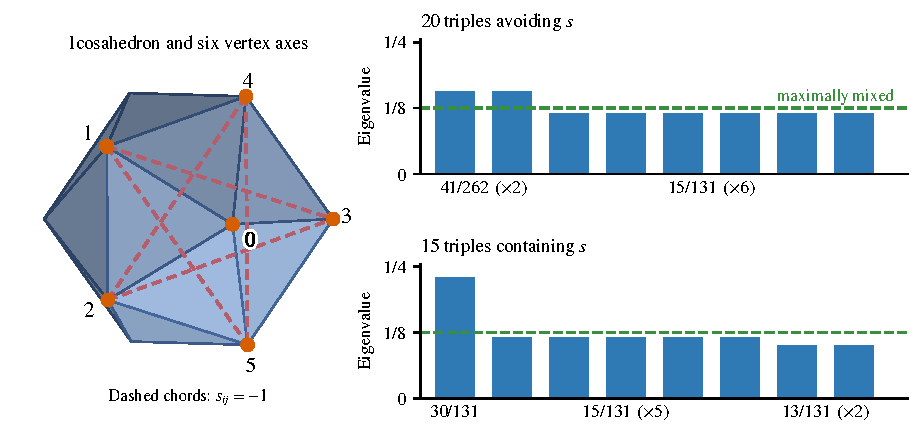
\includegraphics[width=\linewidth]{fig_icosahedron}
\caption{Icosahedral geometry and marginal spectra of $\Psiico=\psi_{37/524}$.
Left: six oriented representatives of the axes through opposite icosahedral vertices label qubits
$0,\ldots,5$; the distinguished seventh qubit $s$ is separate. Dashed chords mark pairs whose amplitude sign
$s_{ij}$ is $-1$. Right: spectra of the $20$ three-qubit marginals avoiding $s$ and the $15$ containing it;
multiplicities in parentheses (the values $(4u)^6,(3u+x)^2$ and $8u,(4u)^5,(u+x)^2$ above at $u=15/524$); every marginal in a class has the spectrum shown. The dashed horizontal line marks the maximally mixed eigenvalue
$1/8$. This state minimises the mean purity over all pure states. The entropy maximiser $\psi_{x_*}$,
$x_*=0.0698\ldots$, is a different member of the same family; its spectra have the same multiplicities, and each
eigenvalue differs from the one shown by less than $10^{-3}$, too little to see at this scale.}
\label{fig:fqe-icosahedral}
\end{figure}

The icosahedron enters through the signs. The matrix $C$ with zero diagonal and entries $s_{ij}$ off it is a symmetric
\emph{conference matrix}: $C^2=5I$. Its eigenvalues are $\pm\sqrt5$, each three times, so $I+C/\sqrt5$ is positive
semidefinite of rank three with unit diagonal. It is therefore the Gram matrix of six unit vectors in $\mathbb R^3$ with
$v_i\cdot v_j=s_{ij}/\sqrt5$: six equiangular lines~\cite{LS} at angle $\arccos(1/\sqrt5)$, which are the axes through opposite
vertices of an icosahedron. The same identity block-diagonalises every two- and three-qubit marginal of $\psi_x$ in
the computational basis, which is how Theorem~\ref{thm:ico} obtains the spectra.

The family is the fixed set of a symmetry group generated by local unitaries, qubit permutations and complex
conjugation (up to signs and phase). Hence a member stationary within the family is stationary on the whole sphere for
the purity, the entropy or any other differentiable functional invariant under these symmetries
(Lemma~\ref{lem:seven-family-symmetric-criticality} of the supplement, which identifies the group).

\paragraph{Why an icosahedron.} An exact purity identity shows why minimising purity selects this geometry. Widen the
family: replace the pair amplitudes $\alpha s_{ij}$ of $\psi_x$ by complex numbers $t_{ij}$ in the $|0\rangle_s$ branch
and by their conjugates in the $|1\rangle_s$ branch. They form a complex symmetric $6\times6$ matrix $Q=(t_{ij})$ with
zero diagonal; put $p_i=\sum_j|t_{ij}|^2$ and $\sigma=\sum_{i<j}|t_{ij}|^2$, so normalisation is $2\sigma+2x=1$. For every
such state the weight-one and weight-three Pauli correlations on the six ordinary qubits cancel between the two branches
(Theorem~\ref{thm:spinflip-double} of the supplement), and (Theorem~\ref{thm:complexsos} of the supplement)
\begin{equation}\label{eq:fqe-complex-sos}
\begin{aligned}
 \pi_3-\frac{121}{917}={}&\frac{(524x-37)^2}{137550}+\frac4{35}\sum_i\Bigl(p_i-\frac\sigma3\Bigr)^2\\
 &+\frac{48}{35}\sum_{i<j}\Bigl(|t_{ij}|^2-\frac\sigma{15}\Bigr)^2+\frac{24}{35}\sum_{i<j}\bigl|(QQ^\dagger)_{ij}\bigr|^2.
\end{aligned}
\end{equation}
At equality $x=37/524$, all $|t_{ij}|$ are equal and the rows of $Q$ are orthogonal: $Q$ is a multiple of a complex
conference matrix of order six, which is unique up to diagonal phases and permutations
(Proposition~\ref{prop:confphase} of the supplement) and is the icosahedral sign pattern above. Minimum purity thus
forces the six rows of pair amplitudes to be orthogonal with equal moduli. The identity is exact only within this
family and does not bound arbitrary states; the global bound is the five-copy certificate of
Theorem~\ref{thm:fqe-seven-purity}, whose equality analysis reduces an arbitrary minimiser to this family and this identity.

\paragraph{Entropy selects a different state.} Since the marginal eigenvalues of $\psi_x$ are affine in $x$, its mean entropy
is explicit: with $f(t)=-t\log_2t$ and $u=(1-2x)/30$,
\[
 E_3(\psi_x)=\tfrac1{35}\bigl[195f(4u)+40f(3u+x)+15f(8u)+30f(u+x)\bigr]
\]
(Appendix~\ref{sec:ico}). It is strictly concave in $x$, and its unique maximum occurs at the root $x_*\in(0,1/2)$ of
\begin{equation}\label{eq:fqe-xstar}
 2^{32}(1-2x)^{15}=3^8(1+8x)^8(1+28x)^7
\end{equation}
(Proposition~\ref{prop:entropy-seven-stationarity} of the supplement),
giving $E_3(\psi_{x_*})=2.965356029\ldots$ bits. This root lies strictly below $37/524$
(Corollary~\ref{cor:ico-entropy-separation}), so $\Psiico$ is not stationary for the entropy, even within the family.
By Theorem~\ref{thm:fqe-seven-purity} no purity minimiser maximises the mean entropy: unlike at four qubits, the two
problems have different solutions. Their objective values are nevertheless very close: $E_3(\Psiico)$ lies only $7.1597\ldots\cdot10^{-6}$ bits
below the maximum, and $\pi_3(\psi_{x_*})$ exceeds $121/917$ by $1.2204\ldots\cdot10^{-6}$ (rigorous interval enclosures).

The marginal moments give a heuristic explanation for this difference; the exact derivative in
Corollary~\ref{cor:ico-entropy-separation} supplies the proof. In the Taylor expansion of $f$ about the mean eigenvalue $1/8$,
the second-moment contribution favours small $\pi_3$, while the positive cubic coefficient favours a large
$b_3=\tfrac1{35}\sum_{|S|=3}\operatorname{tr}\rho_S^3$. At four qubits $M_4$ does both: it minimises $P$ and maximises
the cubic moment $T$ on the slice $P=1$ (Theorem~\ref{thm:fqe-moment}). Along $\psi_x$, instead,
$b_3(\psi_x)=(35008x^3+17328x^2-3084x+709)/31500$ has $b_3'(37/524)=-432/120127<0$ (Appendix~\ref{sec:ico}): moving
$x$ below $37/524$ raises $b_3$ at first order and costs $\pi_3$ only at second order.

The marginal spectra and pair purities of the minimiser agree, to the six digits published, with
those of a seven-qubit state found numerically by Di~Martino, Facchi and Florio~\cite{DMFF18}. This suggests that the two
states are LU-equivalent (Appendix~\ref{sec:ico}); Theorem~\ref{thm:ico} gives an explicit closed-form state.

\paragraph{Copies of the state.} A purity is an expectation value in two copies, and a homogeneous polynomial of
degree $m$ in $|\psi\rangle\langle\psi|$ is an expectation value in $m$ copies. Averaging the projector onto
$\psi^{\otimes m}$ over local unitaries, qubit permutations and complex conjugation gives the \emph{twirled $m$-copy
moment}. Replacing some copies by the spin-flipped state $\tilde\psi=\epsilon^{\otimes n}\bar\psi$ (which differs from $\sigma_y^{\otimes n}\bar\psi$ only by the phase $i^n$),
$\epsilon=i\sigma_y$, gives further positive operators, all linear images of it. Minimising $\pi_3$ over all moment operators subject to these positivity conditions gives lower bounds
that increase with $m$ to the true minimum, a bosonic-extension hierarchy in the spirit of~\cite{DPS}, and close to the copy hierarchy of Yu et al.\ for the pure-state
marginal problem~\cite{YSWNG} (Appendix~\ref{sec:fqe-seven} and Theorem~\ref{thm:spinflip-ppt-hierarchy} of
the supplement). A certificate at level $m$ is an identity
\begin{center}
(objective) $-$ (bound) $=$ a sum of squared norms of linear images of $m$ copies of $\psi$, some spin flipped.
\end{center}
At four qubits $P\ge1$ follows at the two-copy level from Rains' shadow inequalities~\cite{Rains}, and the sextic
identity~\eqref{eq:fqe-remainder} is a three-copy certificate for the different objective $F$ (Appendix~\ref{sec:fqe-seven}). At seven qubits the levels separate: two copies give only the AME value $1/8$, three copies
provably cannot reach $121/917$, four copies provably fall short (numerically by about $7.5\cdot10^{-5}$), and five copies are the first level that attains the sharp purity bound
(Table~\ref{tab:fqe-seven-levels}).

\paragraph{Proof outline for the purity minimum.} The proof has three steps; the entropy proof below repeats them at a
different point of the family.
\begin{enumerate}
\item \emph{Bound.} A five-copy identity writes $\pi_3-121/917$ as a sum of twelve terms, each the expectation value of a
positive operator in five copies of $\psi$, some of them spin flipped, averaged over local unitaries and qubit
permutations. Every term is therefore nonnegative, which gives the bound. Unlike at four qubits, the identity needs
computer assistance: floating-point linear algebra with rigorous error bounds establishes that suitable positive definite
coefficient matrices exist.
\item \emph{Equality moments.} At equality all twelve terms vanish. Their vanishing fixes the averaged five-copy moment of
$\psi$ to that of $\Psiico$ (Theorem~\ref{thm:fivecopy-family-equality} of the supplement): every conjugation-even,
permutation-invariant five-copy invariant of $\psi$ takes its icosahedral value.
\item \emph{Equality state.} A reconstruction theorem (Theorem~\ref{thm:moment-orbit-rigidity} of the supplement) then
shows that $\psi$ differs from $\Psiico$ only by local unitaries and a qubit permutation. Some of these invariants put
$\psi$ in the form of the widened family above, and the identity~\eqref{eq:fqe-complex-sos}
makes the amplitude matrix $Q$ a conference matrix.
With qubit labels fixed, the orbit of $\Psiico$ consists of $42$ LU orbits: $7$ choices of the distinguished qubit times
$6$ inequivalent sign patterns of the conference matrix.
\end{enumerate}
Appendix~\ref{sec:fqe-seven} defines the terms and records the tangent-line step, the invariants used and the sizes of the
computations; Section~\ref{sec:fivecopy} of the supplement gives the full proof.

\paragraph{Proof outline for the entropy maximum.} The proof follows the four-qubit pattern: a polynomial majorant
touching the entropy at the spectra of the maximiser, then a moment certificate. Across the 35 cuts of $\psi_{x_*}$, four
distinct eigenvalues occur. A single one-variable majorant of $-t\log_2t$ sharp on every cut would therefore touch at
four points and need degree at least seven, and hence seven copies (Proposition~\ref{prop:seven-entropy-majorant-degree}
of the supplement). We instead use each marginal $\rho_S$ together
with its spin flip $\widetilde\rho_S=\sigma_y^{\otimes3}\rho_S^T\sigma_y^{\otimes3}$, which is also the marginal of
$\tilde\psi$ on $S$; it has the spectrum of $\rho_S$ but in general different eigenvectors. At $\psi_{x_*}$ the two commute,
and their joint eigenvalue pairs $(\lambda,\mu)$ take only five values. With $u=(1-2x_*)/30$, the cut
eigenvalues of $\psi_{x_*}$ are $\nu_1=3u+x_*$, $\nu_2=8u$, $\nu_3=4u$ and $\nu_4=u+x_*$ (Theorem~\ref{thm:ico}), and the
pairs are $(\nu_3,\nu_3)$, $(\nu_1,\nu_1)$, $(\nu_4,\nu_4)$, $(\nu_2,\nu_3)$ and $(\nu_3,\nu_2)$.
A scalar inequality bounds the average entropy of two eigenvalues by a degree-five polynomial: there is a symmetric
polynomial $H(\lambda,\mu)$ of degree five majorising $\tfrac12[-\lambda\log_2\lambda-\mu\log_2\mu]$, with first-order
contact at those five pairs (Section~\ref{sec:seven-joint-analytic-proof} of the supplement proves it, with exact
one-variable sign checks). For arbitrary marginals the two eigenbases need not coincide. Their squared overlaps
nevertheless form a doubly stochastic matrix, so averaging the scalar inequality with these weights gives, with
$h_{kl}$ the coefficients of $H$,
\[
S(\rho_S)\le
\sum_{k,l}h_{kl}\operatorname{tr}(\rho_S^k\widetilde\rho_S^{\,l}),
\]
even when $\rho_S$ and $\widetilde\rho_S$ do not commute. The right side is a five-copy moment.

It suffices to bound this polynomial for states attaining or exceeding $E_3(\psi_{x_*})$, so the certificate is only
needed on a compact domain containing them, cut out by two technical restrictions (Proposition~\ref{prop:seven-competitor-band}
and Corollary~\ref{cor:seven-entropy-eigen-cap-497} of the supplement). The purity minimum and the entropy--purity slope
for eight eigenvalues give the \emph{purity band} $121/917\le\pi_3<8693/64000$, and
spin-flip compatibility between overlapping cuts caps every marginal eigenvalue at $497/1000$. On this
domain a positive five-copy identity bounds the polynomial by the candidate value $E_3(\psi_{x_*})$
(Theorem~\ref{thm:seven-entropy-localized-identity} of the supplement; Appendix~\ref{sec:fqe-seven} lists its terms).
At equality all its terms vanish, and the equality-moment argument and reconstruction
theorem used for purity identify the orbit (Theorems~\ref{thm:fivecopy-family-equality} and~\ref{thm:moment-orbit-rigidity} of the
supplement).

\paragraph{Stability.} Both optima are quadratically stable: each optimiser is a strict local optimum modulo local
unitaries and phase with an explicit quadratic basin, and compactness extends this to a global lower bound on the objective deficit by a constant
times the squared distance to the orbit under local unitaries and qubit permutations. We do not make the constant explicit (Theorems~\ref{thm:icolocal},
\ref{thm:icoquantbasin}, \ref{thm:entropy-seven-local} and~\ref{thm:entropy-seven-quantbasin} and
Corollary~\ref{cor:seven-global-quadratic} of the supplement).

\paragraph{Comparison with four qubits.} The two sizes differ in the equality set. At four qubits the purity minimum $P=1$ is attained on a positive-dimensional
set, containing $M_4$ and the cluster state, and the entropy needs the cut spectrum to single out $M_4$
(Proposition~\ref{prop:fqe-onecut}). At seven qubits the purity alone selects a single orbit under LU and qubit permutations,
and the two-copy level of the hierarchy is no longer sharp (Section~\ref{sec:fqe-discussion} compares other sizes).

Table~\ref{tab:fqe-four-seven} summarises the common method and the additional constraints needed at seven qubits. The degree rule of
Section~\ref{sec:fqe-entropy_maximum-entropy-bound} explains both majorants: $k=2$ gives the cubic of Section~\ref{sec:fqe-entropy_maximum-entropy-bound}, and the joint
majorant evades $k=4$ by adding the spin-flip variable. It also shows that degree five is the least possible for a joint
majorant. A joint majorant sharp at $\psi_{x_*}$ must touch at the three diagonal pairs $(\lambda,\lambda)$ among its
contacts. On the diagonal it is therefore a majorant of $-t\log_2t$ touching at three distinct points, which needs degree at least five
(Corollary~\ref{cor:seven-joint-degree-five} of the supplement). Within this majorant method five copies are therefore necessary for the entropy; that says nothing about other certificates.

\begin{table}[ht]
\centering\small
\renewcommand{\arraystretch}{1.15}
\begin{tabular}{@{}lll@{}}
\toprule
 & four qubits, $2|2$ cuts & seven qubits, $3|4$ cuts\\
\midrule
mean purity minimum & $\pi_2=1/3$ (two copies) & $\pi_3=121/917$ (five copies)\\
purity equality set & positive-dimensional, contains $M_4$ & one orbit, $\Psiico$\\
entropy maximiser & $M_4$ & $\psi_{x_*}\ne\Psiico$\\
majorant & cubic in $\lambda$, contacts $1/6,1/2$ & degree five in $(\lambda,\mu)$, five contact pairs\\
moment certificate & sextic identity, three copies & certified identity, five copies\\
extra constraints & none & purity band, cap $\lambda\le497/1000$\\
entropy equality & $M_4$ orbit (Theorem~\ref{thm:fqe-entropy-max}) & $\psi_{x_*}$ orbit\\
\bottomrule
\end{tabular}
\caption{The copy-hierarchy method at four and seven qubits. Here $\pi_2=P/3$ and $\pi_3$ are the mean balanced cut
purities. Orbits include local unitaries and qubit permutations; $\mu$ is an eigenvalue of the spin-flipped marginal.}
\label{tab:fqe-four-seven}
\end{table}



\section{Discussion and open problems}\label{sec:fqe-discussion}

\paragraph{Intermediate R\'enyi orders.} Gour and Wallach conjectured that $M_4$ maximises the mean
R\'enyi-$q$ entropy for $q<\alpha_0\approx1.59$ and the cluster states for $q>\alpha_0$, and proved the
cluster-state bound for $q\ge2$~\cite[Fig.~2 and Theorem~12]{GW}; their $\alpha_0$ is the crossing $q_*$ of
Proposition~\ref{prop:fqe-renyi-crossing}, and Corollary~\ref{cor:fqe-renyi-gw} proves the conjecture. For $1<q<2$ a
single-crossing property of individual spectra (Lemma~\ref{lem:fqe-renyi-single-crossing}) transfers two anchor bounds to
all intermediate orders, and Appendix~\ref{sec:fqe-renyi-proofs} gives the argument and the finite checks it uses.

\paragraph{Quantitative stability.} The universal coefficient $1/20$ in
Theorem~\ref{thm:fqe-orbit-stability} is not claimed to be sharp, and whether the critical optimum $C_*$ of
Section~\ref{sec:fqe-stability-summary} holds for all states is open. Numerical tests of locally filtered
critical states have found no smaller $\delta/d^2$
(Remark~\ref{rem:fqe-critical-noncritical} of the supplement). Local filtering does not preserve the entropy deficit,
even though the overlap bound of Theorem~\ref{thm:fqe-global-overlap} holds without a
criticality assumption.

\paragraph{Seven-qubit questions.} The five-copy proofs give sharp purity and
entropy bounds, but an analytic certificate comparable to the four-qubit
sextic identity would better explain the global role of the icosahedral
geometry. The entropy ceiling also holds for mixed-state convex roofs, with equality only for pure states
(Proposition~\ref{prop:seven-mixed-roofs} of the supplement); where the four-qubit argument finds a support vector of
deficient Schmidt rank, the seven-qubit one uses that the optimiser's local-unitary tangent space contains no complex line.

\paragraph{The method.} At both sizes the proof starts from the spectra of the candidate optimiser, builds a
polynomial majorant touching the entropy at those spectra, bounds the required moments by positivity of
multicopy operators with some copies spin flipped, and reads off the equality states from the vanishing
terms. The spin-flip constraints rely on the pseudoreality $\epsilon\bar u\epsilon^{-1}=u$ of $SU(2)$. For $SU(d)$,
$d\ge3$, the defining representation is inequivalent to its conjugate, so this form of the multicopy argument does not extend directly
to qudits.

\paragraph{Purity and entropy at other sizes.} Table~\ref{tab:fqe-other-n} collects what is known. Four qubits is the
smallest size at which the question has content. At five qubits AME states exist, so the mean entropy reaches its
elementary upper bound, exactly at the AME states; their LU classes form a continuum, each LU-equivalent to a point of the
unique $((5,2,3))$ code (five qubits, a two-dimensional code space and distance three), with points identified under a
group of order~24~\cite{Tan}. The minimum purity is
the value of the Rains linear programme~\cite{Rains,HESG}, the two-copy level of the hierarchy, attained by a graph state, at
every $n\le18$ except $7$ and $13$ (Theorems~\ref{thm:lptable}, \ref{thm:fourteenfifteen}, \ref{thm:sixteenseventeen}
and~\ref{thm:eighteen} of the supplement~\cite{Companion}). A graph state is the stabilizer state obtained from
$|+\rangle^{\otimes n}$ by a controlled-$Z$ gate along each edge of a graph on the qubits; every stabilizer state is
locally equivalent to one~\cite{VdN,HEB}, and $C_4$ is locally equivalent to the graph state of the four-vertex path. Seven qubits is the first size at which the two-copy level is
not sharp: the linear-programming value would require the weight distribution of a pure $((7,1,4))_2$ code, which does
not exist~\cite{HGS}. At thirteen qubits it is not sharp either: the three-copy level gives $\min\pi_6\ge0.018171249$, above the
linear-programming value $25/1408$, and an explicit stabilizer state gives $\min\pi_6\le85/4576$, but the exact minimum
is open (Proposition~\ref{prop:thirteeninterval} of the supplement); here the linear-programming value would require a
pure $((13,1,6))_2$ code, which the three-copy bound excludes.

The maximum entropy is known only at the AME sizes
and at four and seven qubits. Elsewhere each purity minimum, or at thirteen qubits its lower bound, gives an explicit
entropy ceiling through a sharp linear inequality: every $d$-dimensional density matrix, $d\ge3$, satisfies
$\log_2d-S(\rho)\ge c_d(d\operatorname{tr}\rho^2-1)$ with $c_d=(d-1)\log_2(d-1)/(d(d-2))$
(Lemma~\ref{lem:seven-entropy-linear-purity} of the supplement). Being linear in the purity, this inequality averages over the
balanced cuts, $E_k\le k-c_{2^k}(2^k\pi_k-1)$, whereas the largest entropy at fixed purity is not concave in the purity and
does not average this way. At thirteen qubits an explicit state also gives $\max E_6>5.8336$
(Corollary~\ref{cor:thirteen-entropy-witness} of the supplement). The ceilings are not attained by the graph-state
purity minimisers. A stabilizer state's marginals are normalised projectors, so unless $n\in\{2,3,5,6\}$ some balanced
marginal is rank-deficient; such a marginal can always be perturbed to raise the entropy at order $t^2|\ln t|$.
Hence no stabilizer state is even a local maximum of the mean balanced entropy
(Corollary~\ref{cor:stabilizer-entropy-noname} of the supplement); in particular neither seven-qubit optimiser is a
stabilizer state.

\begin{table}[htbp]
\centering\small
\begin{tabular}{@{}cccl@{}}
\toprule
$n$ & ideal purity $2^{-k}$ & $\min\pi_k$ & $\max E_k$ (bits)\\
\midrule
2, 3 & $1/2$ & $1/2$ & $1$ (AME)\\
4 & $1/4$ & $1/3$ & $1+\tfrac12\log_23$ (Theorem~\ref{thm:fqe-entropy-max})\\
5 & $1/4$ & $1/4$ & $2$ (AME)\\
6 & $1/8$ & $1/8$ & $3$ (AME)\\
7 & $1/8$ & $121/917$ & $2.96535602947\ldots$ (Theorem~\ref{thm:fqe-seven-entropy})\\
8 & $1/16$ & $3/35$ & $<3.9029$\\
9 & $1/16$ & $1/14$ & $<3.9627$\\
10 & $1/32$ & $1/21$ & $<4.9163$\\
11 & $1/32$ & $1/28$ & $<4.9772$\\
12 & $1/64$ & $5/224$ & $<5.9594$\\
13 & $1/64$ & $[0.018171249,\ 85/4576]$ & $(5.8336,\ 5.9846)$\\
14 & $1/128$ & $331/27456$ & $<6.9702$\\
15 & $1/128$ & $1/104$ & $<6.9874$\\
16 & $1/256$ & $1/156$ & $<7.9800$\\
17 & $1/256$ & $1/208$ & $<7.9928$\\
18 & $1/512$ & $7/2288$ & $<8.9901$\\
\bottomrule
\end{tabular}
\caption{Mean balanced purity and entropy of $n$-qubit pure states. With $k=\lfloor n/2\rfloor$, $\pi_k$ and $E_k$ are
the mean purity and mean von Neumann entropy of the $k$-qubit marginals over all $\binom nk$ subsets of $k$ qubits. The
ideal purity $2^{-k}$ and entropy $k$ are attained exactly at the AME sizes $n=2,3,5,6$. The known purity minima other than
at $n=7$ are Rains linear-programming values attained by graph states (Table~\ref{tab:minima} and
Theorem~\ref{thm:eighteen} of the supplement); at $n=13$ the minimum is open, and the entry is the interval of
Proposition~\ref{prop:thirteeninterval} of the supplement. Single entropy entries without $<$ are exact maxima; entries with $<$
are upper bounds on unknown maxima, the ceilings $k-c_{2^k}(2^k\min\pi_k-1)$ rounded up, with the lower end of the
purity interval in place of $\min\pi_k$ at $n=13$. There the maximum is open; the upper end of its interval is that
ceiling, and the lower end is exceeded by an explicit state (Corollary~\ref{cor:thirteen-entropy-witness} of the
supplement).}
\label{tab:fqe-other-n}
\end{table}

\paragraph{Purity and time reversal.}\label{rem:fqe-spinflip-tradeoff}
A large overlap with the spin-flipped state costs purity: at $n=4$, $\pi_2=\tfrac13+\tfrac16(W_1+\tau)$
(Lemma~\ref{lem:fqe-purity}), and Rains' shadow inequalities give sharp analogues at larger sizes
(Section~\ref{sec:spinflip-tradeoffs} of the supplement~\cite{Companion}).

\paragraph{Formal verification.} The four-qubit maximum, its attainment by $M_4$ and its equality case are formalised in
Lean~4 with Mathlib~\cite{Companion}, together with the moment inequality, the general and critical envelopes, most of the
four-qubit spectral corollaries, the overlap bound with the global orbit-stability estimates, the sharp quadratic
variance bound with the R\'enyi envelope above order one, and the exact
computations for the icosahedral family. Finite checks of two certificates, for the overlap bound and the quadratic
variance bound, use compiled code; the results depending on them inherit that trust assumption, and everything else uses
the Lean kernel alone. The global seven-qubit theorems are not formalised. Section~\ref{sec:fqe-lean} of the supplement
lists the scope, declarations and trust assumptions.

\section*{Use of AI}
All results, documents and scripts were generated by AI agents (mainly Claude Opus and Sonnet 5.5, and OpenAI's GPT 6.1 sol) with human supervision and many cross-checks,
including AI-generated Lean verification of most of the four-qubit results.

\section*{Acknowledgements}
We acknowledge support by the UK STFC grant ST/T000473/1.

\appendix
\section{The sextic from elementary swap contractions}\label{sec:fqe-sextic}

The proof of Theorem~\ref{thm:fqe-moment} has two parts. We first express three tensor contractions as marginal
moments in \eqref{eq:fqe-contractions}. We then eliminate their mixed moment $\Pi_2$ using norms of one-qubit
marginals acting on the state. The derivation uses two-dimensional antisymmetry, partial traces and matrix algebra;
the eleven-type table evaluates the longest contraction. An independent coefficient-by-coefficient check of
\eqref{eq:fqe-remainder} in the sixteen complex amplitudes is also available (SI-1, SI-2,
Appendix~\ref{sec:fqe-verifiers}); it does not use that table.

Write \(R_S=\operatorname{tr}_{S^c}|z\rangle\langle z|\), \(N=\|z\|^2\),
\(P=\sum_{j=2}^4\operatorname{tr}R_{1j}^2\), \(T=\sum_{j=2}^4\operatorname{tr}R_{1j}^3\),
\(\Pi_1=\sum_i\operatorname{tr}R_i^2\) and \(\Pi_2=\sum_{i<j}\operatorname{tr}[R_{ij}(R_i\otimes
R_j)]\). The unnormalised Bloch vectors \(\mathbf r_i=(r_i^a)\) have components \(r_i^a=\langle
z|\sigma_a^{(i)}|z\rangle\); put \(W_1=\sum_i\|\mathbf r_i\|^2=2\Pi_1-4N^2\) and \(F=17NP-12T-12N^3\).

\subsection{One residual tensor and the local moment
map}\label{sec:fqe-sextic_identity-one-residual-tensor-and-the-local-moment-map}

Let \(\epsilon=\begin{pmatrix}0&1\\-1&0\end{pmatrix}=i\sigma_y\) and \(w=z_x\otimes z_y\otimes\tilde z_t\), \(\tilde z=\epsilon^{\otimes4}\bar z\). At one physical site define maps from three qubits to one by \[
L|xyt\rangle=\epsilon_{yt}|x\rangle,\qquad
M|xyt\rangle=\epsilon_{xt}|y\rangle.
\] For each site \(i\), let \(S_i\) symmetrise its three slots (the orthogonal projector onto the symmetric subspace). On the other three sites contract
with \(L\), or with \(L+M\), respectively: \[
U_i=S_i\!\prod_{j\ne i}L_jw,\qquad
V_i=S_i\!\prod_{j\ne i}(L_j+M_j)w.
\] These are ordinary vectors on six qubits (three slots at site \(i\), one at each other site), with the inherited
Hilbert-space norm. Write \(R_i^{(i)}\) for the one-qubit marginal
\(R_i\) acting on qubit \(i\) of \(\mathbb C^{16}\). The exact identity is \[
\boxed{\quad8F=6NW_1+3\sum_i\|V_i-8U_i\|^2+12\sum_{i<j}\bigl\|(R_i^{(i)}-R_j^{(j)})z\bigr\|^2.\quad} \tag{S}
\] It immediately proves the sharp bound \(F\ge\tfrac34NW_1\ge0\). For a product state
\(z=\sqrt N\,a_1\otimes\cdots\otimes a_4\) every \(R_i^{(i)}z=Nz\), so the pair norms vanish, and \(F=3N^3=\tfrac34NW_1\);
the constant \(3/4\) cannot be improved. Proposition~\ref{prop:focus} of the supplement writes \(32F\) as a sum of
site terms alone; (S) keeps the separate \(W_1\) term, which gives this bound and the envelope below.

\emph{How the terms are chosen.} All norms and overlaps of \(U_i,V_i\) are expectation values in \(z^{\otimes3}\) of
slot permutations (Section~\ref{sec:fqe-sextic_identity-the-three-contractions}), so they are polynomials in the
marginal moments. Besides \(N^3,NP,T\), they involve \(\Pi_1\) (equivalently \(W_1\)) and the mixed moment \(\Pi_2\), which
\(F\) does not contain. The pair norms contain exactly this mixed moment. Since \((R_i^{(i)})^2\) acts on qubit \(i\) only,
and a \(2\times2\) matrix of trace \(N\) has \(\operatorname{tr}R^3=\tfrac12(3N\operatorname{tr}R^2-N^3)\),
\[
\bigl\|(R_i^{(i)}-R_j^{(j)})z\bigr\|^2=\operatorname{tr}R_i^3+\operatorname{tr}R_j^3-2\operatorname{tr}[R_{ij}(R_i\otimes R_j)],
\qquad
\sum_{i<j}\bigl\|(R_i^{(i)}-R_j^{(j)})z\bigr\|^2=\tfrac92N\Pi_1-6N^3-2\Pi_2 .
\tag{Pr}\label{eq:fqe-pair-norms}
\]
In \(\sum_i\|V_i-tU_i\|^2\) the coefficient of \(N^3\) is \(-\tfrac43(t-8)(t+4)\). At the root \(t=8\) the \(N^3\)
terms cancel, and the \(\Pi_2\) that remains is removed by the pair norms, leaving the nonnegative multiple
\(6NW_1=18\|U\|^2\); at the other root \(t=-4\) the same elimination leaves a negative multiple of \(NW_1\).

The first tensor is just local polarisation. Contracting the three epsilon pairs gives
\(U_i=-S_i(z_x\otimes(R_i\epsilon^T)_{yt})\). Diagonalise \(R_i\) with eigenvalues \(\lambda,\mu\),
and write \(z=\sqrt\lambda\,|0\rangle|\varphi_0\rangle+\sqrt\mu\,|1\rangle|\varphi_1\rangle\) with orthonormal
\(\varphi_a\) on the remaining sites. Then \(R_i\epsilon^T\) has entries \(-\lambda\) at \((y,t)=(0,1)\) and \(\mu\) at \((1,0)\), the two
Schmidt terms of \(U_i\) are orthogonal, and symmetrising \(|0\rangle(\mu|10\rangle-\lambda|01\rangle)\) and
\(|1\rangle(\mu|10\rangle-\lambda|01\rangle)\) gives \((\mu-\lambda)\) times
\(\tfrac13(|001\rangle+|010\rangle+|100\rangle)\) and \(\tfrac13(|011\rangle+|101\rangle+|110\rangle)\), each of squared norm \(1/3\); the two Schmidt terms carry the weights \(\lambda\) and \(\mu\). Hence \[
\|U_i\|^2=\frac{(\lambda+\mu)(\lambda-\mu)^2}{3}
=\frac N3\|\mathbf r_i\|^2. \tag{U}\label{eq:fqe-local-polarization}
\] Thus the first term in \eqref{eq:fqe-remainder} is \(18\|U\|^2\), an ordinary one-qubit marginal defect. For
nonzero \(z\), equality \(F=0\) forces every \(R_i=NI/2\), hence \(U_i=0\); it then requires \(V_i=0\) for all \(i\).
Section~\ref{sec:fqe-sextic_identity-all-zeros-and-why-the-moment-bound-is-tight} classifies the
remaining zeros.


\subsection{The three contractions}\label{sec:fqe-sextic_identity-the-three-contractions}

Write \(\|U\|^2=\sum_i\|U_i\|^2\), \(\|V\|^2=\sum_i\|V_i\|^2\) and
\(\langle U,V\rangle=\sum_i\langle U_i,V_i\rangle\). We will show \[
\begin{aligned}
\|U\|^2&=(2N\Pi_1-4N^3)/3,\\
\operatorname{Re}\langle U,V\rangle&=(-8N^3-2N\Pi_1+8\Pi_2)/3,\\
\|V\|^2&=(128N^3-226N\Pi_1+136NP+152\Pi_2)/3-32T. \end{aligned}\tag{C}\label{eq:fqe-contractions}
\] These contraction identities imply \eqref{eq:fqe-remainder} by direct substitution:
\(\sum_i\|V_i-8U_i\|^2=\|V\|^2-16\operatorname{Re}\langle U,V\rangle+64\|U\|^2\), and
\eqref{eq:fqe-contractions} turns this into \[
\sum_i\|V_i-8U_i\|^2=\tfrac{136}{3}NP-32T-22N\Pi_1+8\Pi_2 ,
\] in which \(N^3\) has cancelled. Adding twelve times \eqref{eq:fqe-pair-norms} and \(6NW_1=12N\Pi_1-24N^3\) to three
times this gives \(136NP-96T-96N^3=8F\), as claimed. The rest of this subsection
proves \eqref{eq:fqe-contractions}. Every step uses only the invariance of $z^{\otimes3}$ under simultaneous permutations of the
copies, the vanishing of the one-site antisymmetriser and averaging over sites, so \eqref{eq:fqe-contractions} holds as a
linear identity in the twirled three-copy moment with one flipped copy.

\paragraph{Slot permutations.} In this subsection \(p=(12)\), \(q=(13)\), \(r=(23)\) are the
transpositions of the three slots \((x,y,t)\) of one site, acting by permuting the three tensor factors, and \(c\)
is the cycle \(c|a_1a_2a_3\rangle=|a_2a_3a_1\rangle\), with inverse
\(c^{-1}|a_1a_2a_3\rangle=|a_3a_1a_2\rangle\). (Here the letters \(p,q,r\) denote only these
transpositions; in particular \(q\) is not the Tsallis exponent.) Products are composed as operators, right factor first; then \[
cr=q,\qquad pr=c^{-1},\qquad qr=c,\qquad pq=c,\qquad qp=c^{-1}.
\] Antisymmetrising three vectors in dimension two gives zero, so \[
I-p-q-r+c+c^{-1}=0,\qquad S=\tfrac16(I+p+q+r+c+c^{-1})=(p+q+r)/3, \tag{A}\label{eq:fqe-antisym}
\] where \(S\) is the symmetriser of the three slots of one site (a projector).

\paragraph{The kernels.} Let \(\Gamma_3\) denote the partial transpose on slot \(3\), and for an
operator \(A\) on the three slots of a site put
\(\mathfrak t(A)=\bigl[(I\otimes I\otimes\epsilon)^TA(I\otimes I\otimes\epsilon)\bigr]^{\Gamma_3}\). Since
\(\tilde z=\epsilon^{\otimes4}\bar z\), moving \(\epsilon\) from the vector \(\tilde z\) to the operator and
transposing slot \(3\) (which turns \(\bar z\) into \(z\)) gives, for an operator
\(A=\bigotimes_{s=1}^4A_s\) with \(A_s\) acting on the three slots of site \(s\),
\[
\langle w,Aw\rangle=\langle z^{\otimes3},\textstyle\bigotimes_s\mathfrak t(A_s)\,z^{\otimes3}\rangle .
\]
The matrix elements (output \(x'y't'\), input \(xyt\)) of the four needed operators are listed below, with
\(\epsilon_{01}=1=-\epsilon_{10}\); for instance \(L^\dagger L=I\otimes|\epsilon\rangle\langle\epsilon|=I-r\),
where \(|\epsilon\rangle=|01\rangle-|10\rangle\). Conjugation by \(\epsilon\) on slot \(3\) acts on the two
\(\epsilon\)'s that carry the index \(t,t'\) as \(\sum_s\epsilon_{as}\epsilon_{sb}=(\epsilon^2)_{ab}=-\delta_{ab}\);
the two signs cancel, and each such \(\epsilon\)-pair becomes a Kronecker \(\delta\). Then \(\Gamma_3\) exchanges
\(t\) and \(t'\). Hence \[
\begin{aligned}
L^\dagger L&=\delta_{xx'}\epsilon_{y't'}\epsilon_{yt}\ \to\ \delta_{xx'}\delta_{y't}\delta_{yt'}:
&|xyt\rangle&\mapsto|xty\rangle=r,\\
M^\dagger M&=\delta_{yy'}\epsilon_{x't'}\epsilon_{xt}\ \to\ \delta_{yy'}\delta_{x't}\delta_{xt'}:
&|xyt\rangle&\mapsto|tyx\rangle=q,\\
L^\dagger M&=\delta_{x'y}\epsilon_{y't'}\epsilon_{xt}\ \to\ \delta_{x'y}\delta_{y't}\delta_{xt'}:
&|xyt\rangle&\mapsto|ytx\rangle=c,\\
M^\dagger L&=\delta_{xy'}\epsilon_{x't'}\epsilon_{yt}\ \to\ \delta_{xy'}\delta_{x't}\delta_{yt'}:
&|xyt\rangle&\mapsto|txy\rangle=c^{-1}.
\end{aligned}
\] On permutation operators, \(\mathfrak t(I)=I\) and \(\mathfrak t(p)=p\) (slot \(3\) is not involved), while for
\(q=\tfrac12(I+\sum_a\sigma_a\otimes I\otimes\sigma_a)\) and likewise \(r\), the identity
\(\epsilon^T\sigma_a\epsilon=\sigma_y\sigma_a\sigma_y=-\sigma_a^T\) gives \(\mathfrak t(q)=I-q\),
\(\mathfrak t(r)=I-r\). Hence \[
\begin{aligned}
\mathfrak t(S)&=(2I+p-q-r)/3=:S',\\
\mathfrak t((L+M)^\dagger(L+M))&=r+q+c+c^{-1}=-I+p+2q+2r=:K,\\
\mathfrak t(L^\dagger(L+M))&=r+c,\qquad
\mathfrak t(L^\dagger L)=r, \end{aligned}\tag{K}\label{eq:fqe-kernels}
\] using \eqref{eq:fqe-antisym} for \(c+c^{-1}=p+q+r-I\). Since \(S_i^\dagger S_i=S_i\), \[
\|V\|^2=\sum_i\bigl\langle z^{\otimes3},S'_i\textstyle\prod_{j\ne i}K_j\,z^{\otimes3}\bigr\rangle .
\]
The vector \(z^{\otimes3}\) is fixed by every simultaneous slot permutation (the same permutation at all
four sites); these can be multiplied on either side of any word inside its expectation, or used to
conjugate it.

\paragraph{Words and the table.} Expanding \(S'_i\prod_{j\ne i}K_j\) gives a combination of
\emph{words} \((\pi_1,\dots,\pi_4)\), \(\pi_s\in\{I,p,q,r\}\), with \(\pi_s\) acting on the slots of site \(s\).
The coefficient of \(S'\) on \(I,p,q,r\) is \((2,1,-1,-1)/3\) and that of \(K\) is \((-1,1,2,2)\); their
ratios are \((-\tfrac23,\tfrac13,-\tfrac16,-\tfrac16)\). So a word with \(a\) letters \(I\) and
\(\beta_p,\beta_q,\beta_r\) letters \(p,q,r\) has total coefficient (summed over the focused site \(i\)) \[
(-1)^a2^{\beta_q+\beta_r}\bigl[-2a+\beta_p-(\beta_q+\beta_r)/2\bigr]/3 .
\] Conjugation by a global slot permutation (the same permutation on all four sites) permutes the
transposition labels \(p,q,r\) in all six ways and does not change expectations, so the expectation of a word depends only on its \emph{type}
\((a;b,c,d)\): \(a\) is the number of identity letters and \(b\ge c\ge d\) are the multiplicities of the three
transpositions, sorted (together with the placement on the four sites). Let \(\#\) be the number of words of a type (these numbers sum to
\(4^4\)), \(C\) the sum of their coefficients, and \(J\) the mean expectation of the type over its placements
and labellings; then \(\|V\|^2=\sum CJ\). Multiplying every letter on the left by one global transposition \(g\) (written
\(\times g\)) does not change the expectation, and changes \(pq\to c\), \(pr\to c^{-1}\).
The table gives, for each type, a representative word, its reduction, \(J\) and \(C\).
\[
J_*:=\tfrac12(N^3+NP+\Pi_2)-\tfrac34N\Pi_1-\tfrac13T .
\]

{\small
\begin{longtable}{@{}l r l l l r@{}}
\caption{The eleven contraction types in $\|V\|^2$. $\#$ counts the words of each type,
$J$ is their mean expectation over site placements and transposition labels, and $C$ is the sum
of their coefficients, so $\|V\|^2=\sum CJ$. A word acts on the three copies at each of the four
sites; $I$ is the identity and $p,q,r$ are slot transpositions. Types are grouped by the number
of identity letters.}\label{tab:fqe-contractions}\\
\toprule
type & \(\#\) & word & expectation of the word & \(J\) & \(C\) \\
\midrule
\endfirsthead
\multicolumn{6}{@{}l}{\small Table~\ref{tab:fqe-contractions}, continued}\\
\toprule
type & \(\#\) & word & expectation of the word & \(J\) & \(C\) \\
\midrule
\endhead
\bottomrule
\endlastfoot
\((4;0,0,0)\) & 1 & \(IIII\) & \(N^3\) & \(N^3\) & \(-8/3\) \\
\addlinespace
\((3;1,0,0)\) & 12 & \(pIII\) & \(N\operatorname{tr}R_1^2\) & \(N\Pi_1/4\) & \(124/3\) \\
\addlinespace
\((2;2,0,0)\) & 18 & \(ppII\) & \(N\operatorname{tr}R_{12}^2\) & \(NP/3\) & \(-84\) \\
\((2;1,1,0)\) & 36 & \(pqII\) & \(\operatorname{tr}[R_{12}(R_1\otimes R_2)]\) & \(\Pi_2/6\) & \(-136\) \\
\addlinespace
\((1;3,0,0)\) & 12 & \(pppI\) & \(N\operatorname{tr}R_{123}^2=N\operatorname{tr}R_4^2\) & \(N\Pi_1/4\) & \(220/3\) \\
\((1;2,1,0)\) & 72 & \(ppqI\ \overset{\times p}{=}\ IIcp\) & \(\operatorname{tr}[R_{34}^2(R_3\otimes I)]\) & \(\frac{NP+\Pi_2}6-\frac{N\Pi_1}8\) & \(296\) \\
\((1;1,1,1)\) & 24 & \(pqrI\) & see (c) & \(J_*\) & \(64\) \\
\addlinespace
\((0;4,0,0)\) & 3 & \(pppp\ \overset{\times p}{=}\ IIII\) & \(N^3\) & \(N^3\) & \(-20\) \\
\((0;3,1,0)\) & 24 & \(pppq\ \overset{\times p}{=}\ IIIc\) & \(\operatorname{tr}R_4^3\) & \(\frac{3N\Pi_1}8-\frac{N^3}2\) & \(-248/3\) \\
\((0;2,2,0)\) & 18 & \(ppqq\ \overset{\times p}{=}\ IIcc\) & \(\operatorname{tr}R_{34}^3\) & \(T/3\) & \(-48\) \\
\((0;2,1,1)\) & 36 & \(ppqr\ \overset{\times p}{=}\ IIcc^{-1}\) & \(\operatorname{tr}[(R_{34}^{\Gamma})^3]\) & \(J_*\) & \(-16\) \\
\end{longtable}
}

Here \(\operatorname{tr}R_S^k\) is the expectation of the \(k\)-cycle on the sites of \(S\) (and \(\operatorname{tr}R_S^2\)
that of a transposition), as for the usual replica trick, and \(R^\Gamma\) is a partial transpose of a two-qubit matrix on one qubit (see (e)); the entries come from following the index lines
of \(z^{\otimes3}\). The means are obtained as follows.
To make the nontrivial partial-transpose entry explicit, consider the representative
$ppqr$. Multiplication on the left by the global $p$ gives $IIcc^{-1}$.
Trace out sites $1,2$ and write $R=R_{34}$ with entries $R_{ab,a'b'}$.
For partial transpose on the second qubit,
$(R^\Gamma)_{ab,a'b'}=R_{ab',a'b}$, and the opposite cycles give
\[
\begin{aligned}
\langle z^{\otimes3},(IIcc^{-1})z^{\otimes3}\rangle
&=\sum_{a,a',a'';\,b,b',b''}
 R_{ab',a'b}R_{a'b'',a''b'}R_{a''b,ab''}\\
&=\sum_{a,a',a'';\,b,b',b''}
 (R^\Gamma)_{ab,a'b'}(R^\Gamma)_{a'b',a''b''}
 (R^\Gamma)_{a''b'',ab}\\
&=\operatorname{tr}[(R^\Gamma)^3].
\end{aligned}
\]
All six indices run over $\{0,1\}$. This explains why opposite local cycles produce
a partial-transpose moment, whereas equal cycles give $\operatorname{tr}R^3$;
part (e) below evaluates its mean in the marginal invariants.

\begin{enumerate}
\item[(a)] Types \((4;0,0,0)\), \((0;4,0,0)\): \(N^3\) on every word. Types \((3;1,0,0)\), \((1;3,0,0)\), \((0;3,1,0)\):
average over the four sites of \(N\operatorname{tr}R_l^2\) or \(\operatorname{tr}R_l^3\), using
\(\operatorname{tr}R_{123}^2=\operatorname{tr}R_4^2\) for a pure state and
\(\operatorname{tr}R^3=(3N/2)\operatorname{tr}R^2-N^3/2\) for a \(2\times2\) matrix of trace \(N\).
\item[(b)] Types \((2;2,0,0)\), \((0;2,2,0)\): complementary pairs have equal spectra, so over the six pairs
\(\sum_{i<j}\operatorname{tr}R_{ij}^2=2P\) and \(\sum_{i<j}\operatorname{tr}R_{ij}^3=2T\), giving the means
\(NP/3\) and \(T/3\). Type \((2;1,1,0)\): the mean of \(\operatorname{tr}[R_{ij}(R_i\otimes R_j)]\) over the six pairs is \(\Pi_2/6\).
\item[(c)] Type \((1;1,1,1)\): replace the identity letter by \(p+q+r-c-c^{-1}\) (equation~\eqref{eq:fqe-antisym}).
The three transpositions give words of type \((0;2,1,1)\). In the words with \(c\) or \(c^{-1}\), multiplying all letters
by \(c^{-1}\) or \(c\) turns the cycle into \(I\) and permutes the three transpositions, so the type is \((1;1,1,1)\) again.
Thus \(J_{(1;1,1,1)}=3J_{(0;2,1,1)}-2J_{(1;1,1,1)}\): the two types have the same mean.
\end{enumerate}
To evaluate the remaining means, we use the Pauli expansion of a two-qubit matrix, derived for $N=1$ in
Appendix~\ref{sec:fqe-correlation}; the homogeneous forms below follow by scaling.
For the unnormalised \(R_{ij}=\frac14\bigl(NI+\mathbf r_i\!\cdot\!\boldsymbol\sigma_i+\mathbf r_j\!\cdot\!\boldsymbol\sigma_j
+\sum_{a,b}C^{ab}_{ij}\sigma_a\otimes\sigma_b\bigr)\), with \(\mathbf r_i,C_{ij}\) the (unnormalised) expectations
and \(u_{ij}=\|\mathbf r_i\|^2+\|\mathbf r_j\|^2+\|C_{ij}\|_F^2\), \[
\begin{aligned}
&\operatorname{tr}R_{ij}^2=\tfrac14(N^2+u_{ij}),\qquad
\operatorname{tr}[R_{ij}(R_i\otimes R_j)]=\tfrac14\bigl(N^3+N\|\mathbf r_i\|^2+N\|\mathbf r_j\|^2+\mathbf r_i^TC_{ij}\mathbf r_j\bigr),\\
&\operatorname{tr}R_{ij}^3=\tfrac1{16}\bigl(N^3+3Nu_{ij}+6\,\mathbf r_i^TC_{ij}\mathbf r_j-6\det C_{ij}\bigr),\qquad
\operatorname{tr}\bigl[R_{ij}^2(\mathbf r_i\!\cdot\!\boldsymbol\sigma_i\otimes I)\bigr]=\tfrac12\bigl(N\|\mathbf r_i\|^2+\mathbf r_i^TC_{ij}\mathbf r_j\bigr).
\end{aligned}
\]
\begin{enumerate}
\item[(d)] Type \((1;2,1,0)\): writing \(R_i\otimes I=\frac N2I+\frac12\mathbf r_i\!\cdot\!\boldsymbol\sigma_i\otimes I\), the last formula gives the
two-qubit identity \[
\operatorname{tr}[R_{ij}^2(R_i\otimes I)]
=\frac N2\operatorname{tr}R_{ij}^2
+\operatorname{tr}[R_{ij}(R_i\otimes R_j)]
-\frac N2\operatorname{tr}R_j^2 ,
\] since both sides exceed \(\frac N2\operatorname{tr}R_{ij}^2\) by \(\frac14(N\|\mathbf r_i\|^2+\mathbf r_i^TC_{ij}\mathbf r_j)\). Averaging over the twelve ordered pairs
\((i,j)\), whose sums are \(4P\), \(2\Pi_2\), \(3\Pi_1\) for the three terms, gives \(\frac1{12}\bigl(2NP+2\Pi_2-\frac32N\Pi_1\bigr)\), the stated \(J\).
\item[(e)] Type \((0;2,1,1)\): partial transposition of the first qubit (or the second; they differ by a full transpose, which does not change the spectrum) reverses the sign of \(\sigma_y\) there, so
with \(D=\operatorname{diag}(1,-1,1)\) the data become \(\mathbf r_i\to D\mathbf r_i\), \(C_{ij}\to DC_{ij}\) and \(\mathbf r_j\) is unchanged. Hence
\(\mathbf r_i^TC_{ij}\mathbf r_j\) and \(u_{ij}\) are unchanged and \(\det C_{ij}\to-\det C_{ij}\), and the cubic formula above gives
\(\operatorname{tr}[(R_{ij}^{\Gamma})^3]=\operatorname{tr}R_{ij}^3+\tfrac34\det C_{ij}\). Solving the formulas above for
\(\det C_{ij}\) and summing over the six pairs, with \(\sum_{i<j}u_{ij}=8P-6N^2\), \(\sum_{i<j}(\|\mathbf r_i\|^2+\|\mathbf r_j\|^2)=3W_1\) and \(\sum_{i<j}\operatorname{tr}R_{ij}^3=2T\), gives
\(\sum_{i<j}\det C_{ij}=4N^3+4NP+4\Pi_2-6N\Pi_1-\tfrac{16}3T\); hence \(\sum_{i<j}\operatorname{tr}[(R_{ij}^\Gamma)^3]=3(N^3+NP+\Pi_2)-\tfrac92N\Pi_1-2T\), whose mean over six pairs is \(J_*\).
\end{enumerate}
Summing \(CJ\) over the table proves the last line of \eqref{eq:fqe-contractions}.

\paragraph{The other two contractions.} By \eqref{eq:fqe-kernels},
\(\langle U_i,V_i\rangle\) is the expectation of \(S'_i\prod_{j\ne i}(r+c)_j\). Multiply on the right by the global \(r\):
the factors at \(j\ne i\) become \((r+c)r=I+q\), and at \(i\) we get
\(S'_ir_i=\frac13(2r_i-I)+\frac13(c_i^{-1}-c_i)\). Conjugation by the global \(q\) fixes \(q\) and exchanges
\(c\) and \(c^{-1}\), so the expectation of the last term equals its own negative and vanishes. Hence \[
\operatorname{Re}\langle U,V\rangle=\tfrac13\sum_i\Bigl\langle\bigl(2r_i-I\bigr)\prod_{j\ne i}(I+q_j)\Bigr\rangle
=\tfrac13\sum_i\sum_{m=0}^3\ \sum_{A\subseteq\{j\ne i\},\,|A|=m}\bigl\langle(2r_i-I)\,q_A\bigr\rangle ,
\] where \(q_A\) puts \(q\) on the sites of \(A\). There are \(4\binom3m\) pairs \((i,A)\) for each \(m\), and the terms
\(r_iq_A\) have the types \((3;1,0,0)\), \((2;1,1,0)\), \((1;2,1,0)\), \((0;3,1,0)\) for \(m=0,1,2,3\),
and the terms \(I_iq_A\) the types \((4;0,0,0)\), \((3;1,0,0)\), \((2;2,0,0)\), \((1;3,0,0)\), each placement occurring equally often. With
\(J_{(a;b,c,d)}\) the means of the table, \[
\begin{aligned}
\operatorname{Re}\langle U,V\rangle=\tfrac43\Bigl[&2\bigl(J_{(3;1,0,0)}+3J_{(2;1,1,0)}+3J_{(1;2,1,0)}+J_{(0;3,1,0)}\bigr)\\
&-\bigl(J_{(4;0,0,0)}+3J_{(3;1,0,0)}+3J_{(2;2,0,0)}+J_{(1;3,0,0)}\bigr)\Bigr].
\end{aligned}
\] The first bracket is \(\frac12NP+\Pi_2+\frac14N\Pi_1-\frac12N^3\) and the second is \(NP+N\Pi_1+N^3\), which gives
\((-8N^3-2N\Pi_1+8\Pi_2)/3\). Only the first six rows and the row \((0;3,1,0)\) of the table are used.
The same argument for \(\|U\|^2\), with \(L^\dagger L\mapsto r\) on the other sites, leaves
\(\frac13\sum_i\langle 2r_i-I\rangle=\frac13\sum_i(2N\operatorname{tr}R_i^2-N^3)=(2N\Pi_1-4N^3)/3\), agreeing with \eqref{eq:fqe-local-polarization}.
This completes the derivation of \eqref{eq:fqe-contractions}.

\subsection{The critical envelope}\label{sec:fqe-critical-envelope}

On the critical locus $W_1=0$, and the moment bound can be sharpened by the spin-flip invariant. For a critical
normal vector $v$ let $\phi=\sum_kv_km_k\in\mathbb C^4$ be the auxiliary two-qubit vector (Appendix~\ref{sec:fqe-normal-form})
and $\Theta_{\alpha\beta}=\langle\phi|\sigma_\alpha\otimes\sigma_\beta|\phi\rangle$ its Bloch correlation matrix.

\begin{proposition}[critical envelope]\label{prop:fqe-critical-envelope}
Every critical unit four-qubit state satisfies
\[
 \boxed{\quad F=\frac12+\frac74\tau+\frac94\operatorname{perm}\Theta\ \ge\ \tau-\tau^{3/2}.\quad}
 \tag{CE}\label{eq:fqe-critical-envelope}
\]
For $0<\tau\le1$, with $\kappa=\sqrt\tau$, equality holds exactly when
$\Theta=O(\kappa I+(1-\kappa)ss^T)$ with $s\in\{\pm1\}^3/\sqrt3$ and $O$ one of the twelve signed cyclic permutation
matrices whose three signs have product $-1$; such states exist for every $\tau$. Since $P=1+\tau/2$ on this locus, the
cubic moment obeys $T\le\frac5{12}+\frac{17}{12}(P-1)-\frac1{12}(x-x^{3/2})$, $x=2(P-1)$, with equality attained for every
$P\in[1,\tfrac32]$: this is the exact upper boundary of the critical moment region, and it meets the supporting line of
Theorem~\ref{thm:fqe-moment} only at its two ends.
\end{proposition}

\begin{proof}
$F$ and $\tau$ are LU invariant, so take $\psi=G(v)$ with $\|v\|=1$ (Theorem~\ref{thm:fqe-critical-normal-form}).
\emph{The formula.} The twelve magic Bell rays have signed-permutation correlation matrices
(Lemmas~\ref{lem:fqe-critical-correlation}(1) and~\ref{lem:fqe-p1-cuts} of the supplement), so the cut $k\in\mathbb Z/3$ has the four eigenvalues
$(1+\sigma\cdot g^{(k)})/4$, where $g^{(k)}_\beta=\Theta_{\beta+k,\beta}$ is a cyclic diagonal of $\Theta$ and $\sigma$ runs over
the four sign triples with $\sigma_1\sigma_2\sigma_3=-1$. Over these triples $\sum(\sigma\cdot g)=0$,
$\sum(\sigma\cdot g)^2=4|g|^2$ and $\sum(\sigma\cdot g)^3=-24g_1g_2g_3$. The three cyclic diagonals partition the
entries of $\Theta$, and the sum of their products is the even half $e=(\operatorname{perm}\Theta+\det\Theta)/2$ of the
permanent. Hence $P=(3+\|\Theta\|^2)/4$, $T=(3+3\|\Theta\|^2-6e)/16$ and
$F=-\tfrac32+2\|\Theta\|^2+\tfrac92e$. In Schmidt form $\phi=(U\otimes V)(\cos\varphi|00\rangle+\sin\varphi|11\rangle)$,
so $\Theta=R_a\operatorname{diag}(\kappa,-\kappa,1)R_b^T$ with $R_a,R_b\in SO(3)$ the rotations induced by $U,V$ and
$\kappa=\sin2\varphi$ the concurrence of $\phi$, which in the magic basis is $|\sum_kv_k^2|=\sqrt\tau$
by~\eqref{eq:fqe-spin-flip-normal-form}. Thus $\Theta$ has singular values $(1,\kappa,\kappa)$ and $\det\Theta=-\kappa^2$. So $\|\Theta\|^2=1+2\tau$, which gives the formula in~\eqref{eq:fqe-critical-envelope}
and $P=1+\tau/2$ (checks CE-1, CE-2).

\emph{The permanent bound.} Write the polar decomposition $\Theta=OD$, with $O\in O(3)$, $\det O=-1$,
$D=(\Theta^T\Theta)^{1/2}=\kappa I+(1-\kappa)ss^T$ and $ODO^T=\kappa I+(1-\kappa)rr^T$; here $r,s$ are unit top singular
vectors of $\Theta$, the local Bloch directions of $\phi$. For every $3\times3$ matrix $X$,
$\operatorname{perm}X=\langle\omega,X^{\otimes3}\omega\rangle$ with the unit vector
$\omega=6^{-1/2}\sum_\pi e_{\pi1}\otimes e_{\pi2}\otimes e_{\pi3}$. Cauchy--Schwarz gives
\[
 |\operatorname{perm}\Theta|
 =\bigl|\bigl\langle(D^{1/2}O^T)^{\otimes3}\omega,(D^{1/2})^{\otimes3}\omega\bigr\rangle\bigr|
 \le\bigl(\operatorname{perm}(ODO^T)\operatorname{perm}D\bigr)^{1/2}.
\]
For a unit vector $u$ and $y_a=u_a^2$, expanding the permanent by rows,
\[
 \operatorname{perm}\bigl(\kappa I+(1-\kappa)uu^T\bigr)
 =\kappa^3+\kappa^2(1-\kappa)+2\kappa(1-\kappa)^2e_2(y)+6(1-\kappa)^3e_3(y)
 \le\frac{2+3\kappa^2+4\kappa^3}9,
\]
by Maclaurin's inequalities $e_2(y)\le\frac13$, $e_3(y)\le\frac1{27}$ on the simplex (check CE-3); for $\kappa<1$ equality needs
$y=(\frac13,\frac13,\frac13)$. Thus $-\operatorname{perm}\Theta\le(2+3\tau+4\tau^{3/2})/9$, and
$F\ge\frac12+\frac74\tau-\frac14(2+3\tau+4\tau^{3/2})=\tau-\tau^{3/2}$.

\emph{Equality.} Let $\kappa>0$, so $D$ is invertible. Equality forces $r,s\in\{\pm1\}^3/\sqrt3$ when $\kappa<1$, and
equality with a negative sign in Cauchy--Schwarz, $(O^T)^{\otimes3}\omega=-\omega$. As $\omega$ is the symmetric tensor of
$x_1x_2x_3$, this says $x_1x_2x_3$ changes sign under $O^T$; then $O^T$ preserves the union of the coordinate planes, so $O$
is a signed permutation, with sign product $-1$; then $\det O=-\operatorname{sgn}\pi=-1$ makes the permutation $\pi$
even, that is, cyclic (check CE-4). Conversely, for such
$O$ and $s$, $\operatorname{perm}\Theta=\langle(O^T)^{\otimes3}\omega,D^{\otimes3}\omega\rangle=-\operatorname{perm}D$ attains the
bound. Every matrix with singular values $(1,\kappa,\kappa)$ and determinant $-\kappa^2$ has the form
$R_a\operatorname{diag}(\kappa,-\kappa,1)R_b^T$ with $R_a,R_b\in SO(3)$, so it is the correlation matrix of a suitable
$\phi$ in Schmidt form; and every unit $\phi$ is $\sum_kv_km_k$ for a critical $G(v)$.
The moment statement is~\eqref{eq:fqe-critical-envelope} rewritten with $\tau=2(P-1)$ and $F=17P-12T-12$.
\end{proof}

On critical states $W_1=0$, so for unit states \eqref{eq:fqe-critical-envelope} is the critical case of
$F\ge\frac34W_1+\tau-\tau^{3/2}$, which Theorem~\ref{thm:fqe-general-envelope} proves for all states.

\subsection{All zeros and why the moment bound is tight}\label{sec:fqe-sextic_identity-all-zeros-and-why-the-moment-bound-is-tight}

The critical envelope classifies the zeros of $F$. This classification supplements the moment inequality; it is
not used in the proof of Theorem~\ref{thm:fqe-entropy-max}.

\begin{proposition}[complete zero set of the moment inequality]\label{prop:fqe-moment-zeros}
For unit four-qubit states, $F=0$ holds exactly on the two $M_4$ LU orbits and the three LU orbits
of products of Bell pairs, one for each pairing of the labelled qubits.
\end{proposition}

\begin{proof}
A unit zero has $W_1=0$ by Theorem~\ref{thm:fqe-moment}, so it is critical, and since $\tau-\tau^{3/2}>0$ for
$0<\tau<1$, Proposition~\ref{prop:fqe-critical-envelope} leaves $\tau\in\{0,1\}$. At $\tau=1$, $F=0$ is equality in
\eqref{eq:fqe-critical-envelope}, so $\Theta$ is one of the twelve signed cyclic permutation matrices $O$; one cyclic
diagonal then has entries $\pm1$ with product $-1$, and that cut has spectrum $(1,0,0,0)$. The pure cut splits the
state into two two-qubit pure states with maximally mixed one-qubit marginals, that is, two Bell pairs. At $\tau=0$,
$\Theta=rs^T$ with unit $r,s$, and the formula in \eqref{eq:fqe-critical-envelope} reads $F=\frac12+\frac{27}2\prod_ar_as_a$.
Its zero $\prod_ar_as_a=-\frac1{27}$ forces $|r_a|=|s_a|=3^{-1/2}$ by the AM--GM inequality, so every cyclic diagonal
$g^{(k)}$ has entries $\pm\frac13$ with product $-\frac1{27}$ and every cut has spectrum $(\frac12,\frac16,\frac16,\frac16)$;
Proposition~\ref{prop:fqe-onecut} then gives the $M_4$ orbits. Conversely $M_4$, $\overline{M_4}$ and the Bell-pair
products have $F=0$. Section~\ref{sec:sup-sextic-zeros} of the supplement gives an independent proof by a
weighted-variance identity on the critical normal form.
\end{proof}

There is also an elementary way to distinguish the two classes. Let \(D_{1j}\) be the determinant of
the \(1j|\widehat{1j}\) flattening, with qubit indices in increasing order. Every invertible local
transformation multiplies all three determinants by the same factor \(\prod_i(\det A_i)^2\); their
ratios are therefore invariant, even under invertible local filters. Directly, \[
\frac{D_{13}(M_4)}{D_{12}(M_4)}=\frac{1-i\sqrt3}{2},
\] whereas conjugation conjugates this nonreal ratio. Thus the two classes are distinct even under
such filters. LU-inequivalence alone was first proved in~\cite[Prop.~7]{LWB}.

By Proposition~\ref{prop:fqe-moment-zeros}, the supporting line \(17P-12T-12=0\) meets the pure-state
moment region at exactly \((1,5/12)\) and \((3/2,9/8)\); its open line segment is unattainable.

\subsection{The general envelope}\label{sec:fqe-general-envelope}

\begin{theorem}[general envelope and complete equality; exact certificate, FI, FG]\label{thm:fqe-general-envelope}
Every nonzero four-qubit vector satisfies, with $s=z^T\sigma_y^{\otimes4}z$,
\[
 F-\tfrac34NW_1-N|s|^2+|s|^3\ \ge\ \frac{7|s|^2}{8(N+|s|)}\,W_1 .
 \tag{GE}\label{eq:fqe-general-envelope}
\]
For unit states, with $\tau=|s|^2$,
\[
 \boxed{\quad F\ \ge\ \Bigl(\frac34+\frac{7\tau}{8(1+\sqrt\tau)}\Bigr)W_1+\tau-\tau^{3/2}.\quad}
\]
Equality in $F\ge\frac34W_1+\tau-\tau^{3/2}$ holds exactly on fully product states and on the critical
equality family of Proposition~\ref{prop:fqe-critical-envelope}, including its HS endpoint at $\tau=0$ and
Bell-pair-product endpoint at $\tau=1$.
\end{theorem}

The coefficient $\frac78$ of the added $W_1$ term is optimal. On $z=\alpha|0000\rangle+\beta|1111\rangle$ with real
$\alpha,\beta\ge0$, $\alpha^2+\beta^2=1$, one has $s=2\alpha\beta$, $\tau=4\alpha^2\beta^2$, $W_1=4(1-\tau)$ and $F=3+\frac32\tau$, so the boxed bound with $\frac78$ replaced by $C$ leaves the slack
$(\frac72-4C)\tau+(1+4C)\tau^{3/2}$, negative for small $\tau>0$ when $C>\frac78$ (exact check ESH). The proof (Section~\ref{sec:sup-general-envelope} of the supplement) follows $H=F-\frac34NW_1$ along a path of unit states
from a state with $s=0$ to $z$, along which the spin-flip overlap grows from $0$ to $s$; an exact identity for the
derivative of $H$ along this path (exact certificate; checks FI, FG), integrated, gives~\eqref{eq:fqe-general-envelope}, and the zeros of the
remainder give the equality cases.

\section{Critical four-qubit states: an elementary normal form}\label{sec:fqe-normal-form}

The equality proof needs an LU normal form for \emph{critical} states, whose one-qubit marginals are all
maximally mixed. We derive it by elementary linear algebra, including all ranks and singular-value multiplicities. No orbit-closure or Kempf--Ness argument is needed. Exact checks are listed in Appendix~\ref{sec:fqe-verifiers}.

\subsection{Setting}\label{sec:fqe-critical_four_qubit_normal_form-setting}

Let \(m_1,\dots,m_4\) be the magic basis of two qubits, \[
m_1=\tfrac1{\sqrt2}(\lvert00\rangle+\lvert11\rangle),\quad
m_2=\tfrac{i}{\sqrt2}(\lvert01\rangle+\lvert10\rangle),\quad
m_3=\tfrac1{\sqrt2}(\lvert01\rangle-\lvert10\rangle),\quad
m_4=\tfrac{i}{\sqrt2}(\lvert00\rangle-\lvert11\rangle).
\] A four-qubit state is \(\psi=\sum_{j,k}Z_{jk}\,m_j\otimes m_k\) with \(Z\in\mathbb C^{4\times4}\)
(qubits 1,2 index the rows, qubits 3,4 the columns), \(\|Z\|_F=1\). In this basis \(u\otimes u'\in
SU(2)\otimes SU(2)\) acts as a real rotation, \(SU(2)\otimes SU(2)\to SO(4)\) onto, so the local
unitaries act as \(Z\mapsto O_1ZO_2^{T}\), \(O_1,O_2\in SO(4)\). For \(v\in\mathbb C^4\) put \[
G(v)=\sum_{k=1}^4v_k\,m_k\otimes m_k .
\] Expanding the \(m_k\) shows \(G(v)=G_{abcd}\), the family
\(\tfrac{a+d}2(\lvert0000\rangle+\lvert1111\rangle)+\tfrac{a-d}2(\lvert0011\rangle+\lvert1100\rangle)+\tfrac{b+c}2(\lvert0101\rangle+\lvert1010\rangle)+\tfrac{b-c}2(\lvert0110\rangle+\lvert1001\rangle)\)
with \((a,b,c,d)=(v_1,-v_2,v_3,-v_4)\) (CN-2).

\paragraph{Spin flip on the normal form.} The invariant \(\tau=|\psi^T\sigma_y^{\otimes4}\psi|^2\) of
Lemma~\ref{lem:fqe-purity} is LU invariant, because \(u^T\sigma_yu=(\det u)\sigma_y\) for
\(u\in U(2)\): a product unitary multiplies \(\psi^T\sigma_y^{\otimes4}\psi\) by
\(\prod_i\det u_i\). Directly from the definitions, \(\sigma_y^{\otimes2}m_k=s_km_k\) with
\(s=(-,+,-,+)\), and \(m_k^Tm_l=\eta_k\delta_{kl}\) with \(\eta=(+,-,+,-)\) (the \(m_k\) are
orthonormal and real up to the phases \(1,i,1,i\)). Hence
\(m_k^T\sigma_y^{\otimes2}m_l=s_l\eta_k\delta_{kl}=-\delta_{kl}\), and for \(\psi=G(v)\)
\[
\psi^T\sigma_y^{\otimes4}\psi=\sum_{k,l}v_kv_l\,\bigl(m_k^T\sigma_y^{\otimes2}m_l\bigr)^2=\sum_kv_k^2,
\qquad\text{so}\qquad \tau=\Bigl|\sum_kv_k^2\Bigr|^2. \tag{$\tau_G$}\label{eq:fqe-spin-flip-normal-form}
\]

\begin{theorem}[Critical normal form]\label{thm:fqe-critical-normal-form}

For a unit four-qubit state $\psi$ with matrix $Z$ the following are equivalent.

\begin{enumerate}
\item All four one-qubit marginals of $\psi$ equal $I/2$ ($\psi$ is \emph{critical}).
\item $ZZ^\dagger$ and $Z^\dagger Z$ are real matrices. Equivalently, for $Z=X+iY$ with $X,Y$ real,
$XY^T$ and $X^TY$ are symmetric.
\item $Z=O_1\operatorname{diag}(v)\,O_2^T$ with $O_1,O_2\in SO(4)$ and $v\in\mathbb C^4$.
\item $\psi$ is local-unitarily equivalent to $G(v)$ for some $v$ with $\|v\|=1$.

\end{enumerate}
\end{theorem}

\begin{lemma}[Simultaneous real singular values]\label{lem:fqe-real-gram}

For any complex $m\times n$ matrix $Z$, the two Gram matrices $ZZ^\dagger$
and $Z^\dagger Z$ are real if and only if
\[
Z=O_1 D O_2^T,\qquad O_1\in O(m),\quad O_2\in O(n),
\]
where $D$ is a complex rectangular diagonal matrix. This includes all ranks
and multiplicities.
\end{lemma}

\begin{proof} Write \(Z=X+iY\). The Gram conditions are precisely \(XY^T=YX^T\) and \(X^TY=Y^TX\).
Take a real SVD of \(X\) and apply its two orthogonal factors to \(Y\) too. On the nonzero diagonal
of \(X\), write \(d_i>0\). The two symmetry equations give \[
d_iY_{ji}=d_jY_{ij},\qquad d_iY_{ij}=d_jY_{ji},
\qquad (d_i^2-d_j^2)Y_{ij}=0.
\] Thus different positive singular-value blocks do not mix, each equal-value block of \(Y\) is
symmetric, and its entries joining a positive block to either nullspace vanish. Diagonalise each
positive block of \(Y\) by the same real orthogonal transformation on its left and right; this
leaves \(X=dI\) fixed. On the remaining, possibly rectangular nullspace block, take a real SVD of
\(Y\). Both \(X\) and \(Y\) are now diagonal. The converse is immediate from the two Gram products.
\end{proof}

\subsection{Proof of the critical normal form}\label{sec:fqe-critical_four_qubit_normal_form-proof-of-theorem}

\begin{proof}[Proof of Theorem~\ref{thm:fqe-critical-normal-form}]
\textit{Marginals are moment maps.}\label{lem:fqe-moment-map}

In the magic basis the six operators \(i\sigma_a\otimes1\), \(i\,1\otimes\sigma_a\) (\(a=x,y,z\))
have real antisymmetric matrices, and they are linearly independent, hence span \(\mathfrak{so}(4)\)
(CN-1: check of the explicit \(4\times4\) matrices). The reduced state of qubits 1,2 is
\(\rho_{12}=ZZ^\dagger\) in the magic basis. For a real antisymmetric \(L\) and Hermitian
\(H=ZZ^\dagger\), \(\operatorname{tr}(L\,\mathrm{Re}H)=0\), so
\(\langle\sigma\otimes1\rangle=\operatorname{tr}(H(-iL))=\operatorname{tr}(L\,\mathrm{Im}H)\). The
six expectations \(\langle\sigma_a\otimes1\rangle,\langle1\otimes\sigma_a\rangle\) are therefore the
six independent components of the antisymmetric matrix \(\mathrm{Im}(ZZ^\dagger)\) under an invertible
linear change of coordinates, and they vanish iff \(\mathrm{Im}(ZZ^\dagger)=0\). Thus the marginals of qubits 1 and 2
are both \(I/2\) iff \(ZZ^\dagger\) is real. In the same way \(\rho_{34}=(Z^\dagger Z)^T\), so
qubits 3 and 4 are maximally mixed iff \(Z^\dagger Z\) is real. This proves
(1)\(\Leftrightarrow\)(2). (Writing \(ZZ^\dagger=XX^T+YY^T+i(YX^T-XY^T)\) and \(Z^\dagger
Z=X^TX+Y^TY+i(X^TY-Y^TX)\) gives the symmetry form of (2).)

\textbf{(3)\(\Rightarrow\)(2).} \(ZZ^\dagger=O_1\operatorname{diag}(|v_k|^2)O_1^T\) and \(Z^\dagger
Z=O_2\operatorname{diag}(|v_k|^2)O_2^T\) are real.

\textbf{(2)\(\Rightarrow\)(3).} Apply the lemma with \(m=n=4\). If an orthogonal factor has
determinant \(-1\), change its first column's sign and the first diagonal entry's sign; thus both
factors can be taken in \(SO(4)\).

\textbf{(3)\(\Leftrightarrow\)(4).} \((U_{12}\otimes U_{34})\,G(v)\) has matrix
\(O_1\operatorname{diag}(v)O_2^T\) when \(U_{12},U_{34}\) act as \(O_1,O_2\) in the magic basis.
\end{proof}

\subsection{Consequences}\label{sec:fqe-critical_four_qubit_normal_form-consequences}

\begin{enumerate}
\def\labelenumi{\arabic{enumi}.}
\item
  On the unitary slice \(Z=W/2\), the lemma is the real-orthogonal KAK factorisation. Here
\(|v_k|=1/2\) and the \(v_k^2\) are the eigenvalues of \(ZZ^T\).
\item
  The \hyperref[sec:fqe-sextic]{sextic zero classification} and
Proposition~\ref{prop:fqe-onecut} use this theorem.
\end{enumerate}


\section{Correlation geometry of the sextic}\label{sec:fqe-correlation}

We use the notation \(F,P,T,\tau\) of Sections~\ref{sec:fqe-entropy_maximum-purity-identity}
and~\ref{sec:fqe-entropy_maximum-the-sharp-moment-inequality} for a unit pure four-qubit state.

\subsection{Correlation-volume identity}\label{sec:fqe-correlation_geometry-correlation-volume-identity}

For a unit state, write \(r_i^a=\langle\sigma_a^{(i)}\rangle\) and
\(C_{ij}^{ab}=\langle\sigma_a^{(i)}\sigma_b^{(j)}\rangle\), with \(C_{ij}\) a real \(3\times3\)
matrix. Expanding a two-qubit marginal in Pauli matrices, and putting
\(u_j=\|r_1\|^2+\|r_j\|^2+\|C_{1j}\|_F^2\), gives \[
\operatorname{tr}\rho_{1j}^2=\frac{1+u_j}{4},\qquad
\operatorname{tr}\rho_{1j}^3=
\frac{1+3u_j+6r_1^TC_{1j}r_j-6\det C_{1j}}{16}.
\] To see this, write \(\rho_{1j}=\tfrac14(I+X)\) with \(X\) the traceless part, so that
\(\operatorname{tr}\rho^3=\tfrac1{64}(4+3\operatorname{tr}X^2+\operatorname{tr}X^3)\) and
\(\operatorname{tr}X^2=4u_j\). In \(\operatorname{tr}X^3\), the terms with one Pauli matrix on each of the two qubits
in every factor give \(\operatorname{tr}(\sigma_a\sigma_c\sigma_e)\operatorname{tr}(\sigma_b\sigma_d\sigma_f)C^{ab}C^{cd}C^{ef}
=(2i)^2\epsilon_{ace}\epsilon_{bdf}C^{ab}C^{cd}C^{ef}=-24\det C_{1j}\), using
\(\operatorname{tr}(\sigma_a\sigma_c\sigma_e)=2i\epsilon_{ace}\); the terms with one Bloch vector on each qubit and one
factor \(C\) give \(6\cdot4\,r_1^TC_{1j}r_j\) (six orderings); the terms with two Bloch vectors on
one qubit, or three, and those with one Bloch vector and two factors \(C\), are traceless (the last because \(CC^T\) is
symmetric while \(\epsilon_{ace}\) is antisymmetric). Hence \(\operatorname{tr}X^3=24(r_1^TC_{1j}r_j-\det C_{1j})\), which gives the stated formulas.
Lemma~\ref{lem:fqe-purity} implies \(\sum_j u_j=4P-3=1+2(W_1+\tau)\), where
\(W_1=\sum_i\|r_i\|^2\). Substitution yields the compact identity \[
\boxed{\quad 2F=
1+8(W_1+\tau)-9\sum_{j=2}^4
\bigl(r_1^TC_{1j}r_j-\det C_{1j}\bigr).\quad} \tag{CV}\label{eq:fqe-correlation-volume}
\] The sum singles out qubit~$1$ only to label the three balanced cuts $\{1,j\}|\{k,l\}$: by the formulas above each
summand equals $(16\operatorname{tr}\rho_{1j}^3-12\operatorname{tr}\rho_{1j}^2+2)/6$, a function of the cut spectrum
alone, so the right-hand side is permutation invariant. Therefore Theorem~\ref{thm:fqe-moment} is equivalent to an
\emph{oriented correlation-volume monogamy inequality} for three compatible two-qubit marginals.
At \(M_4\) the Bloch vectors and \(\tau\) vanish and each \(\det C_{1j}=-1/27\); at
\(\mathrm{Bell}\otimes\mathrm{Bell}\), \(\tau=1\) and the three determinants are \((-1,0,0)\) up to
ordering. This explains the two tight configurations: the spin-flip invariant compensates for
concentration of the correlation volume in a single Bell pair.

Equation \eqref{eq:fqe-correlation-volume} gives a reduced-state reformulation.
Its nonnegativity still requires the moment inequality. Pairwise density-matrix positivity and known absolute
steering-ellipsoid volume-monogamy bounds do not visibly supply the required \emph{oriented} and
\(\tau\)-sensitive inequality (compare the volume monogamy relation for pure four-qubit states of
Cheng, Milne, Hall and Wiseman~\cite{CMHW}, Eq.~(28): in terms of normalised steering-ellipsoid
volumes \(v_{j|1}=|\det(C_{1j}-r_1r_j^T)|/(1-\|r_1\|^2)^2\) of the ellipsoids that qubit \(1\) steers on
qubit \(j\), it reads \(\sum_j v_{j|1}^{2/3}\le1\), which for \(r_1=0\) is
\(\sum_j|\det C_{1j}|^{2/3}\le1\) and is already strict at \(M_4\), giving \(1/3<1\)). RG-1 and RG-2 (Appendix~\ref{sec:fqe-verifiers}) check the local Pauli
formulas and \eqref{eq:fqe-correlation-volume} exactly.

\paragraph{Replica witness.} Let \(p=(12)\) and \(c=(123)\) permute
the \emph{three copies} of a qubit, and use a subscript \(i\) for the physical qubit on which they
act. The Hermitian replica witness \[
K_{\rm rep}=17\sum_{j=2}^4p_1p_j-6\sum_{j=2}^4(c_1c_j+c_1^{-1}c_j^{-1})-12I
\] satisfies \(F(z)=\langle z^{\otimes3},K_{\rm rep}z^{\otimes3}\rangle\) for unit \(z\) (by the usual
swap/cycle formulas for reduced moments). It is not positive on the
copy-symmetric space. On the sector where all four local triples carry spin \(1/2\),
let \(M\simeq\mathbb C^2\) be the standard \(S_3\) multiplicity space and take the three
diagonal-\(S_3\)-fixed pairings \(\delta_{12}\delta_{34}\), \(\delta_{13}\delta_{24}\),
\(\delta_{14}\delta_{23}\) in \(M^{\otimes4}\). Their Gram matrix has diagonal entries 4 and
off-diagonal entries 2; the matrix of \(K_{\rm rep}\) on these pairings has diagonal entries \(-52\) and
off-diagonal entries 42. The generalised eigenvalues are \(4,-47,-47\) (RG-3, exact). Thus
\(K_{\rm rep}\) is indefinite even on \(\operatorname{Sym}^3((\mathbb
C^2)^{\otimes4})\). By uniqueness of polarisation of a bidegree-\((3,3)\) polynomial, \(F\) cannot
be a sum of squared moduli of \emph{holomorphic} cubic forms in \(z\) alone. This does not contradict \(F(z)\ge0\) on pure-state tensor powers.

\section{Quantitative stability of the maximising LU orbits}
\label{sec:fqe-orbit-stability}

The entropy deficit $\delta(\psi)=E(M_4)-E(\psi)$ controls the
squared Hilbert-space distance to the two HS orbits. The gap identity
\eqref{eq:fqe-entropy-gap} controls $W_1$ and the spin-flip overlap
$\tau$, but both also vanish at cluster states; the sextic moment
defect is needed to distinguish the maximisers.

The defect $Q$ below bounds HS infidelity with sharp coefficient one
(Theorem~\ref{thm:fqe-global-overlap}). This gives a uniform, nonoptimal
entropy-distance bound, while the optimal coefficient on critical
states is known (Theorem~\ref{thm:fqe-orbit-stability};
Appendix~\ref{sec:fqe-critical-orbit-stability}). We also transfer the
bounds to other spectral functionals
(Appendix~\ref{sec:fqe-orbit-consequences}). Complete proofs and
further stability estimates are in
Sections~\ref{sec:fqe-stability-proofs} and~\ref{sec:sup-stability}
of the supplement~\cite{Companion}.
Write
\[
 \mathcal M=\{e^{i\theta}(U_1\otimes\cdots\otimes U_4)\xi:
       U_i\in SU(2),\ \xi\in\{M_4,\overline{M_4}\}\},\qquad
 d(\psi)=\min_{\chi\in\mathcal M}\|\psi-\chi\|.
\]
Thus global phase is included, qubits are labelled, and
$d^2\le2(1-1/\sqrt6)$ for unit states
(Lemma~\ref{lem:fqe-hs-fidelity-floor} of the supplement). Equivalently, if $\Phi(\psi)=\max_{\chi\in\mathcal M}
|\langle\psi,\chi\rangle|^2$, then $d^2=2(1-\sqrt{\Phi})$.
Use $N,P,T,F$ from Theorem~\ref{thm:fqe-moment}, and put
\[
 Q(z)=F(z)+N(P(z)-N^2)=18NP-12T-13N^3,\qquad
 k=\frac{\ln3-1}{2\ln2}>\frac{16}{225}.
\]
This nonnegative homogeneous sextic vanishes on the unit sphere precisely at $\mathcal M$. On unit states also set
$\mathcal D=F+3(W_1+\tau)=F+6(P-1)=Q+5(W_1+\tau)/2$.
The entropy-gap identity \eqref{eq:fqe-entropy-gap} gives
\begin{equation}\label{eq:fqe-orbit-surrogate}
 \delta(\psi):=1+\tfrac12\log_2 3-E(\psi)\ \ge\ k\mathcal D(\psi)\ge k Q(\psi).
\end{equation}
Indeed the left side of \eqref{eq:fqe-entropy-gap} is $3\ln2\,\delta(\psi)$, and its coefficients
$\alpha=15/2-6\ln3$ of $P-1$ and $\beta=3(\ln3-1)/2$ of $F$ satisfy $\alpha>6\beta$, since $\ln3=1.0986\ldots<11/10$.
As $k=\beta/(3\ln2)$, dropping $\Delta_H\ge0$ gives
$\delta\ge(\alpha(P-1)+\beta F)/(3\ln2)\ge k(6(P-1)+F)=k\mathcal D$.
Rational series bounds for $\ln2,\ln3$ give $k>16/225$ (GO-4).

\begin{theorem}[Sharp HS overlap stability]\label{thm:fqe-global-overlap}
For every unit pure four-qubit state,
\begin{equation}\label{eq:fqe-global-overlap-sharp}
 Q(\psi)\ge1-\Phi(\psi)
 \ge\frac{6+\sqrt{6(1+\sqrt{\tau(\psi)})}}{12}\,d(\psi)^2
 \ge\frac{6+\sqrt6}{12}\,d(\psi)^2,\qquad \frac{6+\sqrt6}{12}>\frac7{10}.
\end{equation}
Equality in $Q\ge1-\Phi$ holds on $\mathcal M$ ($Q=0$, $\Phi=1$) and on the three Bell-pair-product LU orbits
($Q=\Phi=1/2$), so the coefficient one is optimal.
\end{theorem}
\noindent[Exact rational certificate, GO-1--GO-3; proof in Section~\ref{sec:fqe-global-overlap} of the supplement.]

\begin{theorem}[Explicit global LU-orbit stability]\label{thm:fqe-orbit-stability}
For every unit pure four-qubit state,
\[
 d(\psi)^2\le\frac{12}{6+\sqrt6}\,Q(\psi),\qquad
 \boxed{\ \delta(\psi)\ge k\,\frac{6+\sqrt6}{12}\,d(\psi)^2\ },\qquad k\,\frac{6+\sqrt6}{12}>\frac1{20}.
\]
For every critical state the optimal bound is $\delta\ge C_*d^2$, with
$C_*\approx0.19058$ (Theorem~\ref{thm:fqe-p1-sharp}).
On an explicit neighbourhood of the two orbits the coefficient improves:
\[
 d(\psi)\le1/20\quad\Longrightarrow\quad
 \delta(\psi)\ge\frac3{10}d(\psi)^2.
\]
Its sharp limiting coefficient is
$c_*=(2-\ln3)/(2\ln2)$, in the precise sense of
\eqref{eq:fqe-entropy-local-sharp}. The power two is optimal.
No optimal global coefficient is claimed; the equality states of
Theorem~\ref{thm:fqe-p1-sharp} show that it is at most $C_*$.
\end{theorem}
\noindent[Uses Theorem~\ref{thm:fqe-global-overlap}; proof in Section~\ref{sec:fqe-stability-proofs} of the supplement.]

The overlap bound is an exact positivity certificate for $Q-(1-\Phi)$ on a $19$-variable closest-orbit normal slice
(Section~\ref{sec:fqe-global-overlap} of the supplement): a degree-six polynomial identity writing it as $277$ rational
Gram forms weighted by the slice's positive constraints, each Gram matrix certified positive by an integer diagonal-dominance test,
plus two explicit nonnegative remainders; the entropy bound then follows from
\eqref{eq:fqe-orbit-surrogate}. The local radius comes from the
transverse quadratic forms of $Q$ and of the entropy at the orbit.
Brierley and Higuchi~\cite{BH} previously proved local maximality of entropy.
The proofs are in Sections~\ref{sec:fqe-stability-proofs} and~\ref{sec:sup-stability} of the supplement.

\begin{table}[htbp]
\centering\small
\begin{tabular}{@{}p{.22\linewidth}p{.22\linewidth}p{.44\linewidth}@{}}
\toprule
Domain & Coefficient in $\delta\ge Cd^2$ & Status and proof \\
\midrule
All unit pure states & $C=1/20$ & Certified, nonoptimal; Theorem~\ref{thm:fqe-global-overlap} and \eqref{eq:fqe-orbit-surrogate}. \\[3pt]
$d\le1/20$ & $C=3/10$ & Explicit local bound; \eqref{eq:fqe-entropy-local-radius} of the supplement. \\[3pt]
$d\to0$ & $c_*=(2-\ln3)/(2\ln2)$ & Sharp limiting coefficient; \eqref{eq:fqe-entropy-local-sharp} of the supplement. \\[3pt]
Critical states & $C=C_*$ & Optimal on the whole critical locus; Theorem~\ref{thm:fqe-p1-sharp}, analytic bounds and interval certificates. \\[3pt]
All unit pure states & $C=C_*$ & Open; the critical equality states give an upper bound on any universal coefficient. \\
\bottomrule
\end{tabular}
\caption{Distance stability: domains, constants and proof methods. The elementary polarisation and
spin-flip defect bounds follow directly from \eqref{eq:fqe-entropy-gap}; they do not yet control $d$.}
\label{tab:fqe-stability-scope}
\end{table}

\subsection{Sharp constants on the critical locus}
\label{sec:fqe-critical-orbit-stability}
A state is critical when all four one-qubit marginals are $I/2$. This locus contains $M_4$, the cluster state and the
Bell-pair products, and on it the constants can be made sharp. Both theorems below are proved in the
supplement~\cite{Companion} (Sections~\ref{sec:fqe-critical-orbit-proof}, \ref{sec:fqe-p1-sharp} and~\ref{sec:fqe-critical-sharp} there).

\begin{theorem}[Sharp critical-state orbit stability]
\label{thm:fqe-critical-orbit-sharp}
For every critical unit pure four-qubit state, with $\Phi,d,Q,k$
as in Appendix~\ref{sec:fqe-orbit-stability},
\begin{align}
 Q(\psi)&\ge\max\{1-\Phi(\psi),\;3/2-2\Phi(\psi)\},
                 \label{eq:fqe-critical-fidelity}\\
 Q(\psi)&\ge\frac{2+\sqrt2}{4}d(\psi)^2,
                 \label{eq:fqe-critical-distance}\\
 \delta(\psi)&\ge k\bigl(\max\{1-\Phi,3/2-2\Phi\}+5\tau/2\bigr)
       \ge k\,\frac{2+\sqrt2}{4}\,d(\psi)^2.
                 \label{eq:fqe-critical-entropy}
\end{align}
The coefficient one in $Q\ge1-\Phi$, and the coefficient
$(2+\sqrt2)/4$ in \eqref{eq:fqe-critical-distance}, are both optimal:
Bell-pair products attain them. The comparison $Q\ge1-\Phi$ holds for all states
(Theorem~\ref{thm:fqe-global-overlap}).
If the critical state also has $\tau=0$, equivalently if $P=1$, then
\begin{equation}\label{eq:fqe-null-critical-sharp}
 \Phi\ge\frac{2+\sqrt3}{6},\qquad
 Q\ge\frac3{4-\sqrt3}(1-\Phi)\ge\frac{3+\sqrt3}{4}d^2.
\end{equation}
These coefficients and the fidelity floor are optimal, attained by cluster states.
\end{theorem}
\noindent[Checks CO-1--CO-3. Uses Theorem~\ref{thm:fqe-global-overlap}; proof in Section~\ref{sec:fqe-critical-orbit-proof} of the supplement.]

\noindent The moment route thus gives the entropy coefficient $k(2+\sqrt2)/4$ on the critical locus. On the slice $P=1$ a critical normal form is described by two auxiliary Bloch vectors
$r,s\in S^2$ (equation~\eqref{eq:fqe-null-critical-bloch} of the supplement), in which Section~\ref{sec:sup-nullsharp} of the
supplement proves a one-parameter sharpening of \eqref{eq:fqe-null-critical-sharp}. The optimal entropy coefficient
on the critical locus is larger. Put $p=\cos^2(\pi/8)=(2+\sqrt2)/4$, $H_{\rm b}(x)=-x\log_2x-(1-x)\log_2(1-x)$ and
\begin{equation}\label{eq:fqe-p1-cstar}
 C_*=\frac{\tfrac12\log_23-\tfrac13\bigl(1+2H_{\rm b}(p)\bigr)}
          {2-\sqrt{(1+1/\sqrt3)(1+\sqrt{2/3})}}
    =0.190578947\ldots
\end{equation}

\begin{theorem}[Sharp entropy stability on the critical locus]
\label{thm:fqe-p1-sharp}
Every critical unit pure four-qubit state satisfies
\[
 \delta(\psi)\ \ge\ C_*\,d(\psi)^2 ,
\]
and equality with $d>0$ holds exactly for states whose critical normal form has
one of the following $144$ Bloch-coordinate pairs, all with $P=1$. In the auxiliary Bloch coordinates $(r,s)\in S^2\times S^2$ of the null-critical normal form they are: one of $r,s$ is a signed
coordinate axis and the other is $(\pm e_b\pm e_c)/\sqrt2$, $b\ne c$ ($6\cdot12$ pairs, twice for the swap).
These pairs attain the bound, so $C_*$ is the optimal coefficient on the critical locus. Consequently every universal coefficient in
$\delta\ge Cd^2$ is at most $C_*$, and the question left open is whether $C_*$ is optimal over all states.
\end{theorem}
\noindent[Interval-certified; proof in Sections~\ref{sec:fqe-p1-sharp} and~\ref{sec:fqe-critical-sharp} of the supplement.]

\noindent The equality states explain the formula~\eqref{eq:fqe-p1-cstar}. For $r=e_1$, $s=(e_2+e_3)/\sqrt2$ one cut is maximally
mixed and the other two have spectrum $(p,p,1-p,1-p)/2$ (Lemma~\ref{lem:fqe-p1-cuts} of the supplement), so the
numerator is the entropy deficit $\delta=1+\frac12\log_23-\frac13\bigl(2+2(1+H_{\rm b}(p))\bigr)$; the closest cube pair gives
$2\sqrt\Phi=\sqrt{(1+1/\sqrt3)(1+\sqrt{2/3})}$, so the denominator is $d^2=2-2\sqrt\Phi$.
The proof represents a critical state by a $3\times3$
correlation matrix in a six-parameter chart, settles $\tau\ge0.36$ analytically, and covers the rest by an
interval-certified bisection together with a local cone lemma at the equality points.

\subsection{Spectral functionals and limitations}
\label{sec:fqe-orbit-consequences}
\begin{corollary}[Spectral-majorant stability]\label{cor:fqe-orbit-spectral}
In Proposition~\ref{prop:fqe-majorant}, suppose $a>0$ and
$\alpha=-b-17a/12>0$. Then
\[
 \mathcal E_f(M_4)-\mathcal E_f(\psi)
 \ge\frac{c_O}{3}\min(\alpha,a/12)d(\psi)^2,\qquad c_O=\frac{6+\sqrt6}{12}.
\]
For critical states, $c_O$ can be replaced by $(2+\sqrt2)/4$.
For $d\le2^{-10}$ the local bound $Q\ge3d^2$ replaces $c_O/3$ by $1$.
In particular this applies to every fixed Tsallis parameter $0<q<2$,
including its von Neumann limit in nats. At $q=2$, the enlarged
maximiser set prevents such stability relative to $\mathcal M$.
The same holds for every defect estimate of this shape: the R\'enyi
defect estimate \eqref{eq:fqe-renyi-defect} in the proof of
Theorem~\ref{thm:fqe-renyi-above-one} of the supplement,
$3m_q\ln2\,(\mathcal E_q(M_4)-\mathcal E_q(\psi))\ge\alpha_q(P-1)+\frac{a_q}{12}F$
with $m_q=2^{-q}+3\cdot6^{-q}$ and $a_q,\alpha_q>0$ the cubic and purity coefficients defined there, gives for $1<q\le5/4$
\[
 \mathcal E_q(M_4)-\mathcal E_q(\psi)
 \ge\frac{c_O\min(\alpha_q,a_q/12)}{3m_q\ln2}\,d(\psi)^2 .
\]
\end{corollary}
\noindent[Uses Theorem~\ref{thm:fqe-global-overlap}.]
\begin{proof} Drop the scalar remainder in \eqref{eq:fqe-spectral}. Since $P\ge1$, $F\ge0$ and $Q=F+P-1$ on unit states,
$\alpha(P-1)+\frac a{12}F\ge\min(\alpha,a/12)\,Q$; this is also the R\'enyi case. Then use $Q\ge c_Od^2$
(Theorem~\ref{thm:fqe-global-overlap}), \eqref{eq:fqe-critical-distance} for critical states, or, for the local
statement, $Q\ge3d^2$ when $d\le2^{-10}$ (Section~\ref{sec:fqe-orbit-local} of the supplement). \end{proof}

\paragraph{Limitations.}
The global coefficient remains a worst-case bound. Bell-pair products have
$F=0$ but $Q=1/2$, and the cluster state has $W_1=\tau=0$ but
$Q=F=1/2$, so neither term of $\mathcal D=F+3(W_1+\tau)$ alone controls the distance. The sharp local entropy
coefficient is $c_*$; the quadratic coefficients of $Q$ at the orbit are $6$ and $20$.
The comparison $Q(\psi)\ge1-\Phi(\psi)$ is sharp (Theorem~\ref{thm:fqe-global-overlap}), but $1-\Phi$ and
$d^2$ are comparable only up to the factor $(1+\sqrt\Phi)/2\in[\frac{6+\sqrt6}{12},1]$, and $\mathcal D\ge Q$ discards the
spin-flip and polarisation terms.

\section{Proofs for R\'enyi, Tsallis and mixed-state entropies}\label{sec:fqe-spectral-proofs}

\begin{proof}[Proof of Corollary~\ref{cor:fqe-tsallis}]The limit \(q\to1\) is the von Neumann entropy bound \emph{in nats} (divide by
\(\ln2\) for bits). For the proof take \(f_q(x)=(x^q-x)/(1-q)\), with \(f_q(0)=0\). On \((0,1)\), \[
f_q'''(x)=q(2-q)x^{q-3}>0,\qquad
f_q^{(4)}(x)=-q(2-q)(3-q)x^{q-4}<0.
\] Thus its Hermite cubic has \(a_q>0\) and majorises \(f_q\), including \(0\) by continuity. Set
\(g(q)=(15-7q)3^{q-1}/(5+3q)\). Direct divided differences give \[
b_q+\tfrac{17}{12}a_q
=\frac{6^{3-q}}{48(1-q)}
\bigl[5+3q-(15-7q)3^{q-1}\bigr]
=\frac{6^{3-q}(5+3q)}{48}\cdot\frac{1-g(q)}{1-q}<0. \tag{T}\label{eq:fqe-tsallis-coefficient}
\] The prefactor is positive, so the sign claim is that \(g>1\) on \((0,1)\) and \(g<1\) on \((1,2)\).
Indeed \(g(0)=g(1)=1\) and \[
(\log g)'=\ln3-\frac{80}{(15-7q)(5+3q)}.
\] Since \((15-7q)(5+3q)=75+10q-21q^2\), and \(16/15<\ln3<5/4\), this derivative is positive at \(q=0\),
increases up to the vertex \(q=5/21\) of the quadratic and then decreases, so it crosses zero exactly once in
\((0,1)\) (it is \(\ln3-\tfrac54<0\) at \(q=1\)) and remains negative on \([1,2)\). Thus \(g>1\) on \((0,1)\)
and \(g<1\) on \((1,2)\), proving the strict sign in \eqref{eq:fqe-tsallis-coefficient} on either
side of \(q=1\). The logarithm bounds follow, for example, from \(\ln3=\sum_{k\ge0}1/((2k+1)4^k)\):
its first two terms give the lower bound \(13/12\), and using \(2k+1\ge3\) in the terms with \(k\ge2\) gives the upper
bound \(13/12+\tfrac13\sum_{k\ge2}4^{-k}=10/9\). At \(q=1\), since \(g(1)=1\), the quotient \((1-g(q))/(1-q)\) tends to \(g'(1)=(\log g)'(1)=\ln3-\tfrac54\),
so the continuous limit is \(b_1+17a_1/12=\tfrac{36\cdot8}{48}(\ln3-\tfrac54)=6\ln3-\tfrac{15}2<0\).
As for the von Neumann entropy, \(f_q^{(4)}<0\) makes the Hermite remainder vanish on \([0,1]\) only at the two nodes, so
equality can also be identified without the zeros of \(F\): \(P=1\) and \(\Delta_f=0\) give every cut the spectrum
\((\tfrac12,\tfrac16,\tfrac16,\tfrac16)\), and Proposition~\ref{prop:fqe-onecut} applies.

\end{proof}

\paragraph{Sharpness of the Tsallis range.} At \(q=2\) the bound is still valid, but equality is not
unique: \(S_2(\rho)=1-\operatorname{tr}\rho^2\) and Lemma~\ref{lem:fqe-purity} give \(\mathcal
E_{S_2}(\psi)=1-P/3\le2/3\), with equality iff all one-qubit marginals are maximally mixed and
\(\tau=0\). The cluster state $C_4$ of the introduction has cut spectra \((1/2,1/2,0,0)\), \((1/4)^4\), \((1/4)^4\), and so also attains \(2/3\) at
\(q=2\). More strongly, \(M_4\) is not a mean Tsallis-\(q\) maximiser for any \(q>2\). The
averaged cut moments are \[
m_q=2^{-q}+3\,6^{-q},\qquad
c_q=(2^{1-q}+2\,4^{1-q})/3,\qquad
m_q-c_q=\frac{2^{-q}}3(1+9\,3^{-q}-8\,2^{-q}).
\] The last parenthesis vanishes at \(q=2\) and has strictly positive derivative
\(8(\ln2)2^{-q}-9(\ln3)3^{-q}\) for \(q\ge2\): indeed \((3/2)^q\ge9/4>9\ln3/(8\ln2)\) follows from
\(4>3\). Therefore \(S_q(C_4)>S_q(M_4)\) for all \(q>2\). This explains why the parameter range
\(0<q<2\) for unique \(M_4\) maximisers ends sharply at 2.

\paragraph{Expanded spectral gap.} In the setting of Proposition~\ref{prop:fqe-majorant}, with $\alpha$ and $\Delta_f$ as in its proof, the purity identity
(Lemma~\ref{lem:fqe-purity}) and the remainder identity~\eqref{eq:fqe-remainder} at \(N=1\), \(z=\psi\), turn
\eqref{eq:fqe-spectral} into the equivalent formula
\[
\begin{aligned}
3\bigl(\mathcal E_f(M_4)-\mathcal E_f(\psi)\bigr)
={}&\left(\frac\alpha2+\frac{a}{16}\right)W_1+\frac\alpha2\tau+\frac a{32}\sum_i\|V_i-8U_i\|^2\\
&+\frac a8\sum_{i<j}\bigl\|(R_i^{(i)}-R_j^{(j)})z\bigr\|^2+\Delta_f,
\end{aligned}\tag{SF+}\label{eq:fqe-spectral-plus}
\]
in which every term is nonnegative. The residual and pair terms sum to $\frac a{12}\bigl(F-\frac34W_1\bigr)$, which
Theorem~\ref{thm:fqe-general-envelope} bounds below by $\frac a{12}(\tau-\tau^{3/2})$.

\paragraph{Tsallis stability.} For \(0<q<2\), with \(\delta_q=\mathcal E_{S_q}(M_4)-\mathcal
E_{S_q}(\psi)\), the identity \eqref{eq:fqe-spectral-plus}, with \(\alpha_q=-b_q-17a_q/12>0\),
and Theorem~\ref{thm:fqe-general-envelope} give
\[
3\delta_q\ge
\left(\frac{\alpha_q}{2}+\frac{a_q}{16}\right)
W_1+\frac{\alpha_q}{2}\tau+\frac{a_q}{12}\bigl(\tau-\tau^{3/2}\bigr).
\] Here \(\alpha_q,a_q>0\) for every fixed \(q\) in this interval (with the von Neumann limit at \(q=1\)), and
\(\tau-\tau^{3/2}\ge0\). At \(q=2\) the bound becomes the identity \(\delta_2=(W_1+\tau)/6\).

\paragraph{Quantitative consequence for von Neumann entropy.} With \(\delta=E(M_4)-E(\psi)\) in bits,
Theorem~\ref{thm:fqe-general-envelope} gives \[
3\ln2\,\delta\ge
\frac{21-15\ln3}{8}W_1
+\Bigl(\frac{15}4-3\ln3\Bigr)\tau+\frac32(\ln3-1)\bigl(\tau-\tau^{3/2}\bigr).
\] Both \(\tau\) terms are nonnegative, and for small \(\tau\) the
coefficient of \(\tau\) rises from \(\frac{15}4-3\ln3\approx0.454\) to \(\frac94-\frac32\ln3\approx0.602\). Dropping $F$ in \eqref{eq:fqe-entropy-gap} gives the simpler joint estimate \[
W_1+\tau
\le\frac{6\ln2}{\tfrac{15}{2}-6\ln3}\,\delta
\approx4.57862\,\delta.
\] Thus near-maximal entropy forces small one-qubit polarisation and spin-flip overlap.
These conditions alone do not identify the state: cluster states also have $W_1=\tau=0$.
Appendix~\ref{sec:fqe-orbit-stability} adds control of the distance to the two HS orbits and transfers it to
other strict spectral majorants.

\begin{proof}[Proof of Corollary~\ref{cor:fqe-convex-roof}]
The ceiling is proved in the main text after the corollary; it remains to show that no mixed state attains it. Fix one \(2|2\) cut. The support of a
mixed \(\rho\) contains independent vectors with \(4\times4\) flattenings
\(A,B\). Their pencil contains a nonzero singular matrix: either a
generator is singular, or both are invertible and the positive-degree
polynomial \(\det(A+tB)\) has a complex root. Let \(\chi\) be the
normalised support vector represented by that matrix. Because \(\rho\)
is positive definite on its support, for some \(p>0\) the operator
\(\rho-p|\chi\rangle\langle\chi|\) is positive. Thus an ensemble for
\(\rho\) can contain \(\chi\) with positive weight. But \(\chi\) has
deficient Schmidt rank, whereas every pure maximiser has full rank on
this cut. Applying the strict pure-state bound to that ensemble makes
the mean of the convex roofs strictly smaller than the ceiling.

For R\'enyi entropies in the stated range, use the pure-state bound of
Corollary~\ref{cor:fqe-renyi-gw} in place of
\eqref{eq:fqe-spectral}; the same support argument proves strictness.
\end{proof}

The same exclusion of mixed maximisers works whenever all pure maximisers have full Schmidt rank on
one fixed square bipartition.

\section{Proofs for R\'enyi orders above one}\label{sec:fqe-renyi-proofs}

The proof separates physical compatibility from a classical entropy problem.
For a triple of four-point spectra, let $p_j$ be the purity of spectrum $j$ and write
\[
 \varepsilon=P-1,\qquad F=17P-12T-12,\qquad
 V_P=\sum_j(p_j-P/3)^2.
\]
Every pure four-qubit state supplies a triple in the relaxation
\[
 \mathcal R=\left\{\varepsilon\ge0,\quad F\ge0,\quad
                  6V_P\le F^2+\tfrac92\varepsilon\right\}.
\]
The first two constraints are the purity and sextic bounds; the third is (QK), Corollary~\ref{thm:fqe-quadratic-variance} of the sharp bound~\eqref{eq:fqe-quadratic-variance}. No spectral cap is imposed.

\subsection{High orders: an elementary bound}\label{sec:fqe-renyi-high-order}
Every order $q\ge2$ is settled by purity alone, with no anchor, crossing or certificate; the rest of this appendix
is needed only for $1<q<2$.

\begin{corollary}[Unrestricted high-order R\'enyi purity deficit]
\label{cor:fqe-renyi-two-up}
For every pure four-qubit state and every $q\ge2$,
\[
\boxed{\quad
\mathcal E_q(\psi)\le\frac53-\frac13\log_2(2P-1)\le\frac53.
\quad}
\tag{R2}\label{eq:fqe-renyi-two-up}
\]
At $q=2$, the first bound is sharp at every $P\in[1,3/2]$ and equality
holds exactly when two of the three cut marginals are maximally mixed.
For $q>2$, equality in the first bound requires and is attained by the
cluster or Bell-pair-product cut spectra. In particular, for all $q\ge2$
the global ceiling $5/3$ has equality exactly at the cluster-type cut
spectra: $(1/2,1/2,0,0)$, $(1/4)^4$, $(1/4)^4$, up to ordering of cuts.
No eigenvalue-cap hypothesis is assumed.
\end{corollary}
\begin{proof}
Put $p_j=\operatorname{tr}\rho_{1j}^2$ and $x_j=4p_j-1\ge0$.
Lemma~\ref{lem:fqe-purity} gives $P=\sum_jp_j\ge1$. Expanding a product
of nonnegative terms yields
\[
64\prod_{j=2}^4p_j=\prod_j(1+x_j)
\ge1+\sum_jx_j=4P-2,
\]
so $\prod_jp_j\ge(2P-1)/32$. Consequently
\[
\mathcal E_2(\psi)=-\frac13\log_2\prod_jp_j
\le\frac53-\frac13\log_2(2P-1).
\]
R\'enyi entropy is nonincreasing in its order, proving the bound for
$q\ge2$. At $q=2$ equality in the product inequality holds exactly
when at most one $x_j$ is positive, equivalently when at least two
cut spectra are uniform-four. The cluster-to-Bell family
\eqref{eq:fqe-quadratic-family} of Section~\ref{sec:fqe-quadratic-certificate}, with cut spectra
$((1+r)/2,(1-r)/2,0,0),(1/4)^4,(1/4)^4$ for $0\le r\le1$, has precisely
the equality form and $P=1+r^2/2$, proving sharpness for every
$P\in[1,3/2]$.

For $q>2$, equality also requires equality in R\'enyi-order
monotonicity on every cut, hence each cut spectrum is uniform on its
support. The two already-uniform-four spectra contribute total purity
$1/2$. Since $P\ge1$, the last uniform support has rank at most two:
rank two gives the cluster pattern, and rank one the Bell-pair-product
pattern. Both attain the displayed bound. Finally the weaker ceiling
$5/3$ requires $P=1$, which excludes the Bell pattern and leaves only
the cluster-type spectra.
\end{proof}


\subsection{Plan of the anchor proof}\label{sec:fqe-renyi-anchor-plan}
\paragraph{Two anchors suffice.}
Set $q_s=1587/1000<q_*<q_u=8/5$. The anchors must bracket $q_*$, because an HS bound transfers only to lower orders
and a cluster bound only to higher ones, and they are rational so that the supporting inequalities are statements
with exact rational data. Since $\mathcal E_q$ decreases in $q$, the cluster bound is easier to prove as $q$ increases towards $q_*$: $q_s$ is the
lower end of the certified enclosure $1587/1000<q_*<1589/1000$ of Proposition~\ref{prop:fqe-renyi-crossing}, and it
exceeds the threshold $q_b$ that the cubic envelope requires
(Corollary~\ref{cor:fqe-renyi-high-f}). The upper anchor $q_u=8/5$, the end of the interval in
that proposition, is a simple order at which the HS supporting inequality has explicit constants
(Lemma~\ref{lem:fqe-hs-polynomial} of the supplement). Theorem~\ref{thm:fqe-renyi-classical}
partitions $\mathcal R$ into just two regions for order transfer:
\[
\begin{array}{c|c|c}
\text{region}&\text{anchor bound}&\text{anchor equality}\\\hline
F<3/20,\quad20\varepsilon+2F<1
 &\mathcal E_{q_u}\le h_{q_u}&\text{three HS spectra}\\
\text{complement in }\mathcal R
 &\mathcal E_{q_s}\le5/3&\text{cluster triple}.
\end{array}
\]
Here $h_q=H_q(1/2,1/6,1/6,1/6)$ and the cluster triple is
$((1/2,1/2,0,0),(1/4)^4,(1/4)^4)$, up to cut order.
Single crossing (Corollary~\ref{cor:fqe-renyi-order-transfer}) transfers an HS
bound to every lower order above one; ordinary order monotonicity transfers
a constant bound to every higher order. Since $h_{q_s}>5/3>h_{q_u}$,
the two anchors give $\mathcal E_q\le\max\{h_q,5/3\}$ for all $q>1$.
With the anchor equality cases, and single crossing strict off HS spectra,
equality is HS below $q_*$, cluster above it, and both at $q_*$. The proof of Corollary~\ref{cor:fqe-renyi-gw} below gives
the order transfer and physical rigidity explicitly. Orders $0<q\le1$
were settled in Section~\ref{sec:fqe-spectral}.

\paragraph{How the anchor proof is organised.}
The subsections below give single crossing, (QV) and (QK), determinant reduction,
the cubic envelope and the Lagrangian dual. Determinant replacement keeps
each cut's second and third moments and does not decrease its entropy, so the
supporting bounds need only two double-root charts, which include spectra
with an eigenvalue above $1/2$. The supplement proves the anchors through the
disjoint partition of Table~\ref{tab:fqe-renyi-coverage} of the supplement, then the supporting
inequalities in order of use.

The physical input (QK) follows from (QV), which has an exact-rational
certificate and an independent analytic proof on critical states (Section~\ref{sec:fqe-critical-quadratic-variance} of the
supplement). The entropy estimates use calculus and explicit polynomial arithmetic, with exact polynomial sign checks.
An independent near-one defect estimate, critical-locus variance refinements and a shorter proof for states with a
rank-two cut, with further purity-controlled bounds, are in Sections~\ref{sec:fqe-renyi-above-one}--\ref{sec:fqe-renyi-filter-limit} of the supplement; the proof here does not use them.

\subsection{The HS--cluster transition}
Put $m_q=2^{-q}+3\,6^{-q}$, so the HS entropy is $h_q=\log_2m_q/(1-q)$.

\begin{proposition}[HS--cluster crossing]
\label{prop:fqe-renyi-crossing}
There is a unique $q_*\in(3/2,8/5)$ satisfying
\[
\frac{\log_2 m_{q_*}}{1-q_*}=\frac53.
\]
For every $q>q_*$, the cluster state has strictly larger mean R\'enyi entropy
than $M_4$; at $q_*$ the two values coincide. Since $1587/1000<q_*<1589/1000$ (RA-4), $q_*$ is the
threshold $\alpha_0\approx1.59$ of the R\'enyi conjecture of Gour and Wallach~\cite[Fig.~2]{GW}. That the two states are the global maximisers below and above $q_*$ is
Corollary~\ref{cor:fqe-renyi-gw}.
\end{proposition}
\begin{proof}
The cluster spectra recalled above give $(1+2+2)/3=5/3$ for every $q>0$.
The R\'enyi entropy of the nonuniform full-support HS spectrum is strictly
decreasing: $g(q)=\ln m_q$ is strictly convex, $g(1)=0$, and its secant slope
$g(q)/(q-1)$ is strictly increasing. Since $1-q<0$ for $q>1$, $h_q>5/3$ if and only if
$m_q<2^{-5(q-1)/3}$. As $m_q=2^{-q}(1+3^{1-q})$, we have
$m_{3/2}<2^{-5/6}$, as $(1+1/\sqrt3)^3=2+10/(3\sqrt3)<4$ reduces to $100<108$; and $m_{8/5}>1/2$, as
$2^{3/5}<47/31<1+3^{-3/5}$ reduces to $8\cdot31^5<47^5$ and $27\cdot16^5<31^5$. So its R\'enyi value crosses $5/3$
strictly between those parameters. Continuity and strict monotonicity finish.
The same monotonicity and the exact enclosures RA-4 of $\log_2m_q$ at $q=1587/1000$ and
$q=1589/1000$ give $h_{1587/1000}>5/3>h_{1589/1000}$, hence $1587/1000<q_*<1589/1000$.
\end{proof}

\subsection{Single crossing in the order}\label{sec:fqe-renyi-single-crossing}

The orders above one are reduced to two anchor orders by a property of single spectra:
as the order increases, the R\'enyi entropy of any four-point spectrum can overtake that of the HS spectrum
at most once, and never falls back below it. For a probability vector $\lambda$ and $q>1$ put
\[
 u_q(\lambda)=\ln\sum_i\lambda_i^q,\qquad v_q(\lambda)=\partial_qu_q(\lambda)=\frac{\sum_i\lambda_i^q\ln\lambda_i}{\sum_i\lambda_i^q},
 \qquad \kappa_q=\frac1q+\frac{\ln3}{\sinh((q-1)\ln3)},
\]
with $0^q\ln0=0$, so that $H_q(\lambda)\ln2=u_q(\lambda)/(1-q)$.
Write $\sigma=(\tfrac12,\tfrac16,\tfrac16,\tfrac16)$ for the HS spectrum.

\begin{lemma}[Single crossing]\label{lem:fqe-renyi-single-crossing}
For every $q>1$ and every four-point probability vector $\lambda$,
\[
 v_q(\lambda)-v_q(\sigma)\le\kappa_q\bigl(u_q(\lambda)-u_q(\sigma)\bigr),
 \tag{SX}\label{eq:fqe-renyi-single-crossing}
\]
with equality only when $\lambda$ is a permutation of $\sigma$.
\end{lemma}

\begin{corollary}[Order transfer]\label{cor:fqe-renyi-order-transfer}
For every four-point spectrum $\lambda$ the function
\[
 G_\lambda(q)=\frac{(q-1)\bigl(H_q(\lambda)-H_q(\sigma)\bigr)}{q\tanh\bigl((q-1)\ln3/2\bigr)}
\]
is nondecreasing on $(1,\infty)$, strictly unless $\lambda$ is a permutation of $\sigma$.
Consequently, for every triple of four-point spectra and $1<q<q_1$:
if $\mathcal E_{q_1}\le h_{q_1}$ then $\mathcal E_q\le h_q$, with equality only when all three spectra are
HS spectra; and if $\mathcal E_{q_1}<h_{q_1}$ then $\mathcal E_q<h_q$.
\end{corollary}
\begin{proof}
Put $U(q)=u_q(\lambda)-u_q(\sigma)$ and $K(q)=\ln q+\ln\tanh((q-1)\ln3/2)$, so that $K'=\kappa_q$ and
$G_\lambda=-e^{-K}U/\ln2$. By \eqref{eq:fqe-renyi-single-crossing}, $(e^{-K}U)'=e^{-K}(U'-\kappa_qU)\le0$, with equality
at an order only for HS. For a triple, the average of $G_{\lambda^{(j)}}(q)$ is a positive multiple of
$\mathcal E_q-h_q$. It increases strictly unless all three spectra are HS.
Its sign at $q_1$ therefore gives the two transfers and the equality statement.
\end{proof}

\begin{proof}[Proof of Lemma~\ref{lem:fqe-renyi-single-crossing}]
Fix $q>1$, and put $s=q-1$, $L=\ln3$, $\beta=q\kappa_q-1=qL/\sinh(sL)>0$ and
$\varphi=v_q-\kappa_qu_q$. We maximise this continuous function on the simplex.

\emph{A maximiser has full support.} On the positive coordinates, with $Z=\sum_i\lambda_i^q$,
\[
 \partial_i\varphi=\frac{g(\lambda_i)}Z,\qquad
 g(x)=x^{q-1}(q\ln x+C),\qquad C=1-qv_q-q\kappa_q.
\]
The derivative in a zero coordinate is zero, since $x^{q-1}\ln x\to0$.
At a maximiser on a face, the positive-coordinate derivatives equal a multiplier $\mu$.
But $\sum_i\lambda_i\partial_i\varphi=1-q\kappa_q=-\beta$, so $\mu=-\beta$.
Moving mass from a positive coordinate to a zero one therefore has derivative $\beta>0$,
contradicting maximality.

\emph{Only one coordinate can be larger.} Since
\[
 g'(x)=x^{q-2}\bigl[(q-1)(q\ln x+C)+q\bigr],
\]
the bracket is strictly increasing, so $g$ decreases then increases and takes each value at most twice.
The Lagrange condition thus gives at most two coordinate values, $a>b>0$.
If both occur, $g(a)=g(b)$ implies $g'(a)>0$.
Two coordinates equal to $a$ would admit the trace-preserving variation $(a+t,a-t)$.
Its first variations of $Z$ and $v_q$ vanish, and its second variation of $\varphi$ is
$2g'(a)/Z>0$, again contradicting maximality.
Thus every maximiser is uniform or a permutation of $(a,b,b,b)$.

\emph{The one-large family.} Parametrise it by
$a=(1+3e^{-z})^{-1}$, $b=ae^{-z}$, $z\ge0$, and put
$w=3e^{-qz}/(1+3e^{-qz})$, $p=3e^{-z}/(1+3e^{-z})$.
Direct differentiation gives, for $z>0$,
\[
 \begin{aligned}
 \varphi(z)&=\beta\ln(1+3e^{-z})-\kappa_q\ln(1+3e^{-qz})-zw,\\
 \varphi'(z)&=\beta(w-p)+qzw(1-w)
             =zw(1-w)\bigl(q-\beta R(z)\bigr),
 \end{aligned}
\]
where the elementary hyperbolic identity
\[
 R(z)=\frac{(e^{sz}-1)(1+3e^{-qz})}{z(1+3e^{-z})}
     =\frac{\sinh(sz)}z+
       \tanh\!\left(\frac{z-L}{2}\right)\frac{\cosh(sz)-1}z
 \tag{SR}\label{eq:fqe-renyi-crossing-ratio}
\]
settles the sign. The function $\sinh(sz)/z$ is strictly increasing for $z>0$,
and the second summand has the sign of $z-L$. Consequently
\[
 R(z)<R(L)=\frac{\sinh(sL)}L=\frac q\beta\quad(0<z<L),\qquad
 R(z)>R(L)\quad(z>L).
\]
Hence $\varphi$ strictly increases up to $z=L$ and strictly decreases afterwards.
This also excludes the uniform endpoint $z=0$.
Its unique maximum is $z=L$, namely $\sigma$, proving both the inequality and its equality case.
\end{proof}

\subsection{The universal quadratic variance bound}\label{sec:fqe-quadratic-certificate}
For $0\le r\le1$ the critical normal-form vector $v=(\sqrt{(1+r)/2},\,i\sqrt{(1-r)/2},\,0,\,0)$
(Appendix~\ref{sec:fqe-normal-form}) has cut spectra
\[
\bigl((1+r)/2,(1-r)/2,0,0\bigr),\qquad(1/4)^4,\qquad(1/4)^4,
\tag{QF}\label{eq:fqe-quadratic-family}
\]
since its two nonzero components are in quadrature. This \emph{cluster-to-Bell family} joins the cluster
state ($r=0$) to a product of two Bell pairs ($r=1$).


\begin{theorem}[Sharp quadratic purity variance]
\label{thm:fqe-sharp-quadratic-variance}
Every unit pure four-qubit state satisfies
\[
\boxed{\qquad F^2+3P(P-1)\ge6V_P,
\qquad V_P=\sum_{j=2}^4(p_j-P/3)^2.\qquad}
\tag{QV}\label{eq:fqe-quadratic-variance}
\]
Equality holds along the whole cluster-to-Bell family \eqref{eq:fqe-quadratic-family}, so the
coefficient $3$ cannot be decreased.
\end{theorem}
\noindent[Exact-rational certificate, QVA.]

\begin{corollary}[Quadratic purity variance]
\label{thm:fqe-quadratic-variance}
Every unit pure four-qubit state satisfies
\[
\boxed{\qquad F^2+\frac92(P-1)\ge6V_P.\qquad}
\tag{QK}\label{eq:fqe-quadratic-variance-proved}
\]
Equality holds exactly for HS cut spectra, cluster cut spectra, or products
of two Bell pairs, up to ordering of cuts and eigenvalues.
The coefficient $9/2$ cannot be decreased, and the coefficient $6$ cannot
be increased while retaining $9/2$.
\end{corollary}
\begin{proof}[Proofs in outline]
On critical states Proposition~\ref{prop:fqe-critical-quadratic-variance} of the supplement
proves (QV) by a joint-cut analytic argument, and an elementary box bound on the purities proves it whenever
$F\ge3/2-P$. The certificate proves it for all states at once. Homogenised by $N=\lVert z\rVert^2$, the
defect of (QV) is a qubit-symmetric, conjugation-even local-unitary invariant of bidegree $(6,6)$ that
vanishes at HS and cluster; such invariants form an $83$-dimensional space, and $83$ explicit
Gaussian-integer states determine its elements (Section~\ref{sec:fqe-invariant-dimensions} of the supplement).
Ninety-five six-copy covariants, built from $z$ and its spin flip and vanishing at HS and cluster, have squared
norms in that space. With positive integers $q_i$ and $D$, the certificate reads
$2D\,(F^2+3P(P-1)-6V_P)=\sum_iq_i\lVert\Phi_i\rVert^2$ for unit states; its homogeneous
form is~\eqref{eq:fqe-qv-allstate-sos} of the supplement. That homogeneous identity holds at the $83$ states, hence everywhere.
Every term on the right is nonnegative.
For the corollary, the defect of (QK) exceeds that of (QV) by $3(P-1)(3/2-P)\ge0$ on $1\le P\le3/2$, and the
purity box makes (QK) strict above $3/2$; equality is then analysed at $P=1$ by
Proposition~\ref{prop:fqe-critical-variance} of the supplement and at $P=3/2$ by the purity box, which leaves purities
$(1,\tfrac14,\tfrac14)$ and hence products of two Bell pairs. The family \eqref{eq:fqe-quadratic-family} fixes both coefficients.
The complete proofs are in Section~\ref{sec:sup-qk} of the supplement~\cite{Companion}
(exact rational certificate; checks QVA-1--QVA-3, QG-1, QG-3, SD-4).
\end{proof}

\subsection{Determinant reduction for four-point spectra}
\label{sec:fqe-renyi-determinant}

\begin{lemma}[Determinant monotonicity at fixed second and third moments]
\label{lem:fqe-renyi-determinant}
For $1<q<2$, let $\lambda,\lambda'$ be four-point spectra with the same second moment $p$ and third moment $t$.
If $\prod_i\lambda_i<\prod_i\lambda'_i$, then $H_q(\lambda)<H_q(\lambda')$.
Consequently, at fixed $p$ and $t$, the maximum of $H_q$ is attained at a spectrum of one of the two types
\[
(a,b,c,c)\quad\text{or}\quad(a,a,b,c),
\qquad a\ge b\ge c\ge0,
\tag{DM}\label{eq:fqe-renyi-double-root}
\]
including their degenerations.
\end{lemma}
\begin{proof}[Proof idea]
Write $e_k$ for the elementary symmetric polynomials of the eigenvalues and $d=\prod_i\lambda_i$. Newton's identities fix $e_1,e_2,e_3$, so $\prod_i(\lambda_i+s)$ depends on the spectrum only through $d$; a
Stieltjes representation of $x^q$ then shows that $\sum_i\lambda_i^q$ decreases in $d$, and a spectrum of maximal
determinant has a repeated outer pair. The complete proof is in Section~\ref{sec:sup-determinant} of the supplement~\cite{Companion}.
\end{proof}


\begin{corollary}[Six-variable classical reduction]
\label{cor:fqe-renyi-six-variable}
Let three four-component probability vectors be constrained by any
conditions involving only their total second and third moments $P,T$
and the sum of their squared second moments
$U=\sum_jp_j^2$. For every $1<q<2$, the supremum of their mean
R\'enyi entropy is unchanged if each cut is required to have one
of the spectral forms \eqref{eq:fqe-renyi-double-root}.
Up to permutation of cuts, only four patterns need be considered:
$k=0,1,2,3$ cuts with two largest equal, the others with two
smallest equal. Each cut has two free real spectral parameters.
In particular, this reduction is exact for the classical relaxation
$P\ge1$, $F=17P-12T-12\ge0$, and
$F^2+\tfrac92(P-1)\ge6(U-P^2/3)$.
Theorem~\ref{thm:fqe-renyi-classical} bounds this relaxation at the two anchor orders; with
Corollary~\ref{cor:fqe-renyi-order-transfer} and order monotonicity this gives the envelope on it for $q>1$.
\end{corollary}
\begin{proof}
At fixed $p_j,t_j$ for each cut, replacing that spectrum by one of
maximum determinant preserves $P,T,U$ and thus all the stated
constraints. Lemma~\ref{lem:fqe-renyi-determinant} shows that this
replacement cannot decrease any cut entropy. The two forms in (DM)
have two free coordinates after the trace constraint. The cut
permutation symmetry reduces the eight form choices to four.
\end{proof}

\subsection{A sharp cubic R\'enyi bound from binary grouping}
\label{sec:fqe-renyi-cubic-bound}

Binary grouping gives an independent entropy bound that will control the region of large moment slack. Set
\[
q_b=\frac{4\ln2}{4\ln2-1},\qquad
r_b=q_b-1=\frac1{4\ln2-1},\qquad
\frac32<q_b<\frac{313}{200}<\frac{1587}{1000}=q_s.
\tag{BT}\label{eq:fqe-binary-threshold}
\]
Thus $q_b/(r_b\ln2)=4$ and $1/2<r_b<1$.
The bounds on $q_b$ follow from three terms of the atanh series:
$56/81+2/1215<\ln2<1123/1620<3/4$.

\begin{lemma}[Binary grouping]
\label{lem:fqe-renyi-grouping}
For any finite probability vectors $u,v$ and $0\le a\le1$, set
$w=a^2(3-2a)$. Then
\[
H_{q_b}(au,(1-a)v)
\le4a(1-a)+wH_{q_b}(u)+(1-w)H_{q_b}(v).
\tag{BG}\label{eq:fqe-renyi-grouping}
\]
For $0<a<1$, equality holds exactly when $a=1/2$ and
$H_{q_b}(u)=H_{q_b}(v)$.
In particular $H_q(a,1-a)\le4a(1-a)$ holds for every $a$ if and only if
$q\ge q_b$; its equality cases are $a=0,1/2,1$.
\end{lemma}
\begin{proof}
Write $q=q_b$, $r=r_b$, $L=\ln2$ and
$h(w)=-w\ln w-(1-w)\ln(1-w)$.
The log-sum inequality gives, for positive $A,B$,
$\ln(A+B)\ge w\ln A+(1-w)\ln B+h(w)$.
Apply it with $A=a^q2^{-rH_q(u)}$ and
$B=(1-a)^q2^{-rH_q(v)}$. The required assertion follows if
\[
J(a):=q\{w\ln a+(1-w)\ln(1-a)\}+h(w)+4rL a(1-a)\ge0.
\]
The function $J$ is symmetric about $1/2$, and
$J(1/2)=J(1)=0$, with the latter understood by continuity.
Since $w-a=a(1-a)(2a-1)$ and $4rL=q$, differentiation cancels the
terms outside the derivative of $w$:
\[
J'(a)=6a(1-a)\left(q\ln\frac a{1-a}-\ln\frac w{1-w}\right).
\]
For $a>1/2$, put $t=a/(1-a)>1$. Then
\[
\frac w{1-w}=t\,T_2(t),\qquad T_2(t)=\frac{t(t+3)}{3t+1},
\qquad \operatorname{sgn}J'(a)=\operatorname{sgn}\{r\ln t-\ln T_2(t)\}.
\]
The function $s\mapsto\ln T_2(e^s)$ is strictly convex for $s>0$, since
\[
\left(t\frac d{dt}\right)^2\ln T_2(t)
=\frac{24t(t^2-1)}{(t+3)^2(3t+1)^2}>0.
\]
Its derivative starts at $1/2$ and tends to $1$.
Consequently $\ln T_2(e^s)-rs$ starts at zero with negative derivative,
is strictly convex, tends to $+\infty$, and has exactly one further zero.
Thus $J$ increases and then decreases between its zero endpoints $1/2,1$;
it is strictly positive in between. Symmetry proves $J\ge0$ throughout.
Equality in the log-sum inequality at $a=1/2$ requires $A=B$,
which is precisely the stated entropy condition.

Taking both conditional vectors pure proves the binary bound at $q_b$;
order monotonicity proves it for every $q\ge q_b$ with the same equality
cases. Necessity follows as $a=\epsilon\downarrow0$:
$H_q(\epsilon,1-\epsilon)=q\epsilon/((q-1)\ln2)+o(\epsilon)$,
whereas $4\epsilon(1-\epsilon)=4\epsilon+O(\epsilon^2)$.
Orders $q\le1$ are excluded by monotonicity from any $1<q<q_b$.
\end{proof}

\begin{proposition}[Sharp cubic entropy bound]
\label{prop:fqe-cubic-bound}
For every four-point probability vector $\lambda$ and every $q\ge q_b$,
\[
H_q(\lambda)\le\frac{10}3-6p+\frac83t
=4e_2(\lambda)+8e_3(\lambda),\qquad
p=\sum_i\lambda_i^2,\quad t=\sum_i\lambda_i^3.
\tag{CB}\label{eq:fqe-cubic-bound}
\]
The threshold $q_b$ is necessary for a bound valid on the entire simplex.
Equality occurs exactly at pure, uniform-two and uniform-four spectra.
\end{proposition}
\begin{proof}
By order monotonicity it suffices to take $q=q_b$.
Group the entries as
$\lambda=(au,a(1-u),(1-a)v,(1-a)(1-v))$.
For $0<a<1$, Lemma~\ref{lem:fqe-renyi-grouping} and its binary consequence give
\[
H_q(\lambda)\le4a(1-a)
+4a^2(3-2a)u(1-u)+4(1-a)^2(1+2a)v(1-v).
\]
The right side is exactly $4e_2+8e_3$, by expanding across the two groups.
If $a=0$ or $1$ the assertion is the binary bound.
The identity with $(p,t)$ follows from Newton's identities and $\sum\lambda_i=1$.
For equality with $0<a<1$, grouping forces $a=1/2$ and equal conditional
entropies; binary equality then makes both conditional spectra pure or
both uniform-two. This gives uniform-two or uniform-four. The boundary
case also permits a pure spectrum. Each such spectrum stays an equality
at every order, and all other spectra are strict already at $q_b$.
The binary restriction proves sharpness of the threshold.
\end{proof}

\begin{corollary}[Analytic cubic envelope]
\label{cor:fqe-renyi-high-f}
Every triple of four-point probability vectors satisfies, for every $q\ge q_b$,
\[
\mathcal E_q\le\frac53-\frac{20}{27}(P-1)
-\frac2{27}(F-1/2).
\tag{HC}\label{eq:fqe-renyi-high-f}
\]
In particular $\mathcal E_q\le5/3$ whenever $20(P-1)+2F\ge1$.
Equality in the $5/3$ ceiling holds exactly at a permutation of
$((1/2,1/2,0,0),(1/4)^4,(1/4)^4)$.
No quadratic variance bound or physical compatibility is required.
\end{corollary}
\begin{proof}
Sum \eqref{eq:fqe-cubic-bound} over the three cuts, substitute
$T=(17P-12-F)/12$, and divide by three.
Equality in the ceiling requires $20(P-1)+2F=1$ and equality in all three
scalar bounds. Each cut is then pure, uniform-two or uniform-four, with entropy
$0$, $1$ or $2$ at every order, and a mean of $5/3$ forces exactly one uniform-two and two
uniform-four spectra; these have $P=1$, $F=1/2$ and attain $5/3$ at every order.
\end{proof}

\subsection{An exact Lagrangian dual for the classical relaxation}
\label{sec:fqe-renyi-covering}

We now prove the anchor-order bounds used with Corollary~\ref{cor:fqe-renyi-order-transfer}.
The argument uses a classical relaxation of the cut-spectrum constraints: three four-point probability vectors
$\lambda^{(2)},\lambda^{(3)},\lambda^{(4)}$ with
$p_j=\sum_i(\lambda^{(j)}_i)^2$, $t_j=\sum_i(\lambda^{(j)}_i)^3$, $P=\sum p_j\ge1$,
$F=17P-12T-12\ge0$ ($T=\sum t_j$), and the quadratic bound \eqref{eq:fqe-quadratic-variance-proved}.
The cut spectra of every physical state form such a triple (Lemma~\ref{lem:fqe-purity}, Theorem~\ref{thm:fqe-moment},
Corollary~\ref{thm:fqe-quadratic-variance}). Write $\varepsilon=P-1$, $U=\sum p_j^2$,
$f_j=17p_j-12t_j$, and $\mathcal E_q=\frac13\sum_jH_q(\lambda^{(j)})$ in bits.

\begin{lemma}[Lagrangian dual bound]\label{lem:fqe-dual}
For $\theta=(\alpha,\beta,\gamma)\in\mathbb R^2\times[0,\infty)$ put
\[
\Lambda_\theta(\lambda)=H_q(\lambda)+\alpha(p-\tfrac13)+\beta(f-4)-\gamma(p^2-\tfrac19),
\qquad
\ell_\theta(\varepsilon,F)=\alpha\varepsilon+\beta F-\frac\gamma6\Bigl(F^2+\frac{17}2\varepsilon+2\varepsilon^2\Bigr).
\]
For every triple of the relaxation, $\sum_jH_q(\lambda^{(j)})\le\sum_j\Lambda_\theta(\lambda^{(j)})-\ell_\theta(\varepsilon,F)$.
The function $\ell_\theta$ is concave, so on a rectangle its minimum is attained at a corner.
\end{lemma}
\begin{proof}
$\sum_j(p_j-\frac13)=\varepsilon$, $\sum_j(f_j-4)=F$ and $\sum_j(p_j^2-\frac19)=U-\frac13$, hence
$\sum_jH_q=\sum_j\Lambda_\theta-\alpha\varepsilon-\beta F+\gamma(U-\frac13)$. The quadratic bound reads
$6U\le F^2+\frac92\varepsilon+2P^2$, i.e.\ $U-\frac13\le\frac16(F^2+\frac{17}2\varepsilon+2\varepsilon^2)$, and $\gamma\ge0$.
\end{proof}

\begin{lemma}[Sharp third-moment bound at fixed purity]\label{lem:fqe-third-moment}
If a four-point probability vector has purity $p=\frac14+x$, then $0\le x\le\frac34$ and
$\bigl|t-\frac1{16}-\frac34x\bigr|\le x^{3/2}/\sqrt3$.
The upper bound is attained only at the one-large spectrum
$((1+3s)/4,(1-s)/4,(1-s)/4,(1-s)/4)$, up to permutation,
where $s=\sqrt{4x/3}$. The lower bound is attained precisely at its
one-small counterpart when $x\le1/12$; at $x=0$ both are uniform.
\end{lemma}
\begin{proof}
The vectors with given $p$ form a round two-sphere $\{\lambda=\frac14\mathbf1+w:\ \sum w_i=0,\ |w|^2=x\}$
of radius $\sqrt x$. Optimising on the whole sphere gives a valid bound
even when it extends outside the simplex. On it $t=\frac1{16}+\frac34x+\sum w_i^3$; critical points of the cubic
$\sum w_i^3$ have at most two distinct coordinates, namely the patterns $(3,1)$ and $(2,2)$.
The pattern $(2,2)$ has $\sum w^3=0$, and the patterns $(z,z,z,-3z)$ with $12z^2=x$ give
$\sum w^3=-24z^3=\mp x^{3/2}/\sqrt3$.
The upper extremiser has three entries $(1-s)/4\ge0$ for every $x\le3/4$;
the lower has smallest entry $(1-3s)/4\ge0$ exactly when $x\le1/12$.
\end{proof}

\paragraph{Exact contact identities.}
Write $c_1=(1/2,1/2,0,0)$ and $c_2=(1/4)^4$.
Their $(H_q,p,f,p^2)$ values, independent of $q$, are
$(1,1/2,11/2,1/4)$ and $(2,1/4,7/2,1/16)$.
Consequently, with $\Lambda^\star_i=\Lambda_\theta(c_i)$,
\[
\Lambda^\star_1=1+\frac\alpha6+\frac32\beta-\frac5{36}\gamma,
\qquad \Lambda^\star_2=2-\frac\alpha{12}-\frac\beta2+\frac7{144}\gamma,
\qquad \Lambda^\star_1+2\Lambda^\star_2-\ell_\theta(0,1/2)=5,
\tag{DC}\label{eq:fqe-dual-contact}
\]
since $\ell_\theta(0,1/2)=\beta/2-\gamma/24$.
\begin{theorem}[Two R\'enyi anchors]
\label{thm:fqe-renyi-classical}
Let $q_s=1587/1000$ and $q_u=8/5$. Every triple satisfying $P\ge1$, $F\ge0$ and
\eqref{eq:fqe-quadratic-variance-proved} obeys one of the following.
\begin{enumerate}
\item If $F\ge3/20$ or $20\varepsilon+2F\ge1$, then $\mathcal E_{q_s}\le5/3$, with equality only at a permutation of
$(c_1,c_2,c_2)$.
\item Otherwise $\mathcal E_{q_u}\le h_{q_u}$, with equality only when all three spectra are HS spectra.
\end{enumerate}
\end{theorem}
\begin{proof}[Proof outline]
The cubic envelope first removes $20\varepsilon+2F\ge1$.
On the residual, $\varepsilon<1/20$ and every $p_j<11/20$.
For $F<3/20$ use the HS supporting inequality at $q_u$.
For $3/20\le F\le11/25$ use the strict dual band at $q_s$.
The remaining region lies near the cluster triple: the capped cubic bound
handles cuts with $p_j\le47/100$, and the sliver bound handles the unique
cut above that threshold. Table~\ref{tab:fqe-renyi-coverage} and
Section~\ref{sec:sup-renyi-classical-proof} of the supplement~\cite{Companion}
give the complete partition, summation and equality argument.
\end{proof}


\begin{proof}[Proof of Corollary~\ref{cor:fqe-renyi-gw}]
For $0<q<1$ use Corollary~\ref{cor:fqe-renyi}, and for $q=1$ use Theorem~\ref{thm:fqe-entropy-max}.
For $q>1$, the three cut spectra of $\psi$ form a triple of the relaxation
(Lemma~\ref{lem:fqe-purity}, Theorem~\ref{thm:fqe-moment} and Corollary~\ref{thm:fqe-quadratic-variance}); recall
$q_s<q_*<q_u$ and that $\mathcal E_q$ and $h_q$ decrease in $q$.

In case (1) of Theorem~\ref{thm:fqe-renyi-classical}, $\mathcal E_{q_s}\le5/3<h_{q_s}$. Corollary~\ref{cor:fqe-renyi-order-transfer}
gives $\mathcal E_q<h_q$ for $1<q\le q_s$, and $\mathcal E_q\le\mathcal E_{q_s}\le5/3$ for $q\ge q_s$. So
$\mathcal E_q\le\max\{h_q,5/3\}$, strictly for $q<q_*$; for $q\ge q_*$ equality forces $\mathcal E_{q_s}=5/3$, hence the
cluster-type triple.

In case (2), Corollary~\ref{cor:fqe-renyi-order-transfer} gives $\mathcal E_q\le h_q$ for $1<q\le q_u$, with equality only
for three HS spectra, and $\mathcal E_q\le\mathcal E_{q_u}\le h_{q_u}<5/3$ for $q\ge q_u$. As $h_q<5/3$ for $q>q_*$, equality
occurs only for $q\le q_*$ and three HS spectra.

Three HS spectra imply $P=1,F=0$, so Proposition~\ref{prop:fqe-onecut} gives the two HS LU orbits.
A physical state with triple $(c_1,c_2,c_2)$ has two maximally mixed cut marginals;
Proposition~\ref{prop:fqe-two-flat-rigidity} identifies it with the cluster endpoint of
\eqref{eq:fqe-quadratic-family}.
\end{proof}

\begin{remark}[Scope of the relaxation]\label{rem:fqe-renyi-covering-scope}
The classical relaxation uses only $P\ge1$, $F\ge0$ and (QK); no joint purity bound, spectrum cap or four-tangle information.
It is needed only at the two anchor orders: Corollary~\ref{cor:fqe-renyi-order-transfer} acts cut by cut and needs no
compatibility at all.
The multiplier $\beta$ may have either sign; the dual has no gap on the sliver only after the third-moment link of
Lemma~\ref{lem:fqe-third-moment} (a constant $\theta$ on a fixed $(\varepsilon,F)$ cell fails there).
The equality classification uses the same strict local bounds as the inequality;
it requires no additional covering.
\end{remark}



\subsection{A spectral cap from spin flip}
\label{sec:fqe-spectral-spinflip}

The following bound controls the part of a cut spectrum above $1/2$
directly by two-copy quantities. It holds for every pure state, not only on
the critical locus, and needs neither a four-qubit normal form nor a
polynomial certificate.
Write $x_+=\max\{x,0\}$ and use the Hilbert--Schmidt norm throughout.

\begin{proposition}[Spectral spin-flip bound]
\label{prop:fqe-spectral-spinflip}
For every unit pure four-qubit state and every balanced cut $A|A^c$,
\begin{equation}\label{eq:fqe-spectral-spinflip}
 \boxed{\quad
 (2\lambda_{\max}(\rho_A)-1)_+^2
 \le \tau+\frac12W_1
 =2(P-1)-\frac12W_1\le2(P-1).
 \quad}
\end{equation}
Both coefficients on the first right-hand side are optimal. In particular,
$P=1$ forces every balanced eigenvalue to be at most $1/2$.
\end{proposition}

The matrix inequality behind the proposition holds in every bipartite
dimension. The two vectors below need only have the same Schmidt
coefficients; their Schmidt bases may be unrelated.

\begin{lemma}[Overlap and marginal mismatch]
\label{lem:fqe-isospectral-overlap}
Let $\psi,\phi$ be unit bipartite pure states with common squared Schmidt
coefficients $\lambda_1\ge\cdots\ge\lambda_n\ge0$. Let
$\rho_A,\rho_B$ and $\sigma_A,\sigma_B$ be their marginals. Then
\begin{equation}\label{eq:fqe-isospectral-overlap}
 |\langle\psi,\phi\rangle|^2+
 \frac12\bigl(\|\rho_A-\sigma_A\|_F^2+
                    \|\rho_B-\sigma_B\|_F^2\bigr)
 \ge (2\lambda_1-1)_+^2.
\end{equation}
For each common Schmidt spectrum with $\lambda_1\ge1/2$, the bound is
attained by changing the sign of every Schmidt term except the first.
\end{lemma}

\begin{proof}
The case $\lambda_1\le1/2$ is immediate. Assume $\lambda_1>1/2$.
Pad the coefficient matrices with zeros if the local dimensions differ,
and choose Schmidt bases for $\psi$. Its coefficient matrix is
$D=\operatorname{diag}(\sqrt{\lambda_i})$; write $W$ for that of $\phi$.
Thus $WW^\dagger$ and $W^\dagger W$ have eigenvalues $\lambda_i$.
Put
\[
 \Lambda=D^2,\qquad r=1-\lambda_1,\qquad d=2\lambda_1-1,
 \qquad S=\operatorname{diag}(0,r-\lambda_2,\ldots,r-\lambda_n).
\]
The entries of $S$ are nonnegative and increasing. Trace rearrangement
therefore gives, for $R=WW^\dagger$ and for $R=W^\dagger W$,
\begin{equation}\label{eq:fqe-isospectral-rearrange}
 \operatorname{tr}(SR)\ge
 \sum_{i=2}^n(r-\lambda_i)\lambda_i
 =r^2-\sum_{i=2}^n\lambda_i^2.
\end{equation}
Indeed, diagonalising $R$ expresses its diagonal as a doubly stochastic
average of permutations of the decreasing vector $(\lambda_i)$; pairing
it with the increasing diagonal of $S$ is minimised in the displayed order.

Define the quadratic form
\[
 \mathcal B_D(W)=\|W\|_F^2+|\operatorname{tr}(DW)|^2
       -\operatorname{tr}\bigl(\Lambda(WW^\dagger+W^\dagger W)\bigr).
\]
Its useful lower bound has an explicit positive remainder. Let
$W_{\rm t}=(W_{ij})_{i,j\ge2}$ and
$t=\sum_{i=2}^n\sqrt{\lambda_i}W_{ii}$, so $\operatorname{tr}(DW)=\sqrt{\lambda_1}W_{11}+t$. Since
$\Lambda+S=rI+dE_{11}$, with $E_{11}$ the first matrix unit, and $1-2r=d$, the left side below is
$d\bigl(\|W_{\rm t}\|_F^2-|W_{11}|^2\bigr)+|\sqrt{\lambda_1}W_{11}+t|^2$; for $r>0$, completing the square in
$W_{11}$ with $\lambda_1-d=r$ gives
\begin{equation}\label{eq:fqe-isospectral-calibration}
 \begin{split}
 \mathcal B_D(W)-\operatorname{tr}\bigl(S(WW^\dagger+W^\dagger W)\bigr)
 ={}&d\left(\|W_{\rm t}\|_F^2-\frac{|t|^2}{r}\right)
       +\frac{|rW_{11}+\sqrt{\lambda_1}t|^2}{r}\ge0.
 \end{split}
\end{equation}
Cauchy--Schwarz gives
$|t|^2\le r\sum_{i\ge2}|W_{ii}|^2\le r\|W_{\rm t}\|_F^2$.
This proves positivity without any condition on $W$.
When $r=0$, the remainder is simply $\|W_{\rm t}\|_F^2\ge0$.

Apply~\eqref{eq:fqe-isospectral-rearrange} twice to obtain
\[
 \mathcal B_D(W)\ge
 2\left(r^2-\sum_{i=2}^n\lambda_i^2\right).
\]
Set $c_2=\sum_i\lambda_i^2$. In these coordinates
$\langle\psi,\phi\rangle=\operatorname{tr}(DW)$, $\rho_A=\Lambda$, $\sigma_A=WW^\dagger$,
and $\rho_B,\sigma_B$ are the transposes of $\Lambda,W^\dagger W$. Since
$\operatorname{tr}(WW^\dagger)^2=\operatorname{tr}(W^\dagger W)^2=c_2$, the mismatch terms
are $2c_2-2\operatorname{tr}(\Lambda WW^\dagger)$ and
$2c_2-2\operatorname{tr}(\Lambda W^\dagger W)$. With $\|W\|_F^2=1$, the left-hand
side of~\eqref{eq:fqe-isospectral-overlap} is therefore
$\mathcal B_D(W)-1+2c_2$. Its lower bound is
$2r^2+2\lambda_1^2-1=d^2$, as required. Taking
$W=\operatorname{diag}(\sqrt{\lambda_1},-\sqrt{\lambda_2},\ldots,
-\sqrt{\lambda_n})$ proves sharpness.
\end{proof}

\begin{proof}[Proof of Proposition~\ref{prop:fqe-spectral-spinflip}]
Apply Lemma~\ref{lem:fqe-isospectral-overlap} to
$\phi=\widetilde\psi=\sigma_y^{\otimes4}\overline\psi$.
Spin flip preserves every Schmidt spectrum and
$|\langle\psi,\widetilde\psi\rangle|^2=\tau$.
For a two-qubit marginal on sites $i,j$, Pauli expansion gives
\[
 \rho_{ij}-\widetilde\rho_{ij}
 =\frac12\left(\mathbf r_i\cdot\boldsymbol\sigma\otimes I
              +I\otimes\mathbf r_j\cdot\boldsymbol\sigma\right),
 \qquad
 \|\rho_{ij}-\widetilde\rho_{ij}\|_F^2
 =\|\mathbf r_i\|^2+\|\mathbf r_j\|^2.
\]
Thus the two marginal mismatch terms add to $W_1/2$.
The purity identity gives the remaining equalities and inequality
in~\eqref{eq:fqe-spectral-spinflip}.

For sharpness take
$\psi=(a|00\rangle+b|11\rangle)_{12}\otimes
(|00\rangle+|11\rangle)_{34}/\sqrt2$, with real $a,b\ge0$ and
$a^2+b^2=1$. On $12|34$, the left side is one, while
$\tau=4a^2b^2$ and $W_1=2(a^2-b^2)^2$, so equality holds throughout.
The choices $a=b$ and $b=0$ force respectively the coefficients of
$\tau$ and $W_1$ to be at least $1$ and $1/2$.
\end{proof}

Equation~\eqref{eq:fqe-spectral-spinflip} supplies a fully analytic quantum
compatibility constraint. The separate-cut bounds do not by themselves
replace the quadratic variance certificate: SCB-5 gives exact classical spectra
satisfying all three caps and even $F\ge\tau$ (hence the critical
envelope~\eqref{eq:fqe-critical-envelope}) but violating (QK), so compatibility
between the three cut spectra still matters.


\subsection{Quantitative rigidity of two maximally mixed cuts}
\label{sec:fqe-renyi-two-flat}

\begin{proposition}[Crossed purity costs and two-flat rigidity]
\label{prop:fqe-two-flat-rigidity}
Let $\psi$ be any unit pure four-qubit state. Fix a balanced cut $k$,
write its ordered spectrum as
$\lambda_1\ge\lambda_2\ge\lambda_3\ge\lambda_4\ge0$,
and put
\[
\Delta_k=\sum_{j\ne k}(p_j-1/4),\qquad
p_j=\operatorname{tr}\rho_{1j}^2.
\]
If $\lambda_1\ge1/2$, then
\[
\boxed{\quad
\Delta_k\ge\frac14W_1+
2(\lambda_2\lambda_3+\lambda_2\lambda_4+
\lambda_3\lambda_4)
\ge\frac14W_1+(\lambda_3+\lambda_4)^2.\quad}
\tag{TF}\label{eq:fqe-two-flat}
\]
The first inequality is sharp for every chosen spectrum with
$\lambda_1\ge1/2$. On the critical locus, equality holds exactly when
all nonzero squares of the other normal-form amplitudes have a phase
opposite to the square of the largest amplitude. The noncritical
sharpness family in Proposition~\ref{prop:fqe-spectral-spinflip} also
attains the first inequality.

Consequently, whenever \emph{two} balanced cuts of a pure
four-qubit state have maximally mixed marginals $(1/4)^4$,
the third has Schmidt rank at most two. Up to local
unitaries and a permutation of the qubits, every such
state belongs to the attained cluster-to-Bell family
\eqref{eq:fqe-quadratic-family}. In particular the exact
R\'enyi envelope of Proposition~\ref{prop:fqe-renyi-rank-two} of the supplement
applies for all $q>0$.
\end{proposition}
\begin{proof}
The purity identity and Proposition~\ref{prop:fqe-spectral-spinflip} give
\[
2\Delta_k
=2(P-p_k-1/2)
=W_1+\tau-(2p_k-1)
\ge\frac12W_1+(2\lambda_1-1)^2-(2p_k-1).
\]
Using $\sum_i\lambda_i=1$ gives
\[
(2\lambda_1-1)^2-(2p_k-1)
=4(\lambda_2\lambda_3+\lambda_2\lambda_4+
\lambda_3\lambda_4).
\]
This proves the first bound. Since
$\lambda_2\ge(\lambda_3+\lambda_4)/2$,
the second follows by dropping the nonnegative
$\lambda_3\lambda_4$ term.
On the critical locus, write the chosen spectrum as $\lambda_i=|w_i|^2$
in the normal form, so $\tau=|\sum_iw_i^2|^2$.
The bound is then the reverse triangle inequality, with exactly the stated
opposite-phase equality condition. Choosing those phases realises every
ordered spectrum with $\lambda_1\ge1/2$, proving sharpness.

Suppose now two cuts have purity $1/4$. Already one
maximally mixed two-qubit cut forces all four one-qubit
marginals to be $I/2$ by purity of complementary
reductions. If $k$ is the remaining cut, then
$p_k=P-1/2=1/2+\tau/2\ge1/2$. Since
$p_k=\sum_i\lambda_i^2\le\lambda_1$, the hypothesis
$\lambda_1\ge1/2$ holds. The first bound and
$\Delta_k=0$ force at most one among
$\lambda_2,\lambda_3,\lambda_4$ to be nonzero.
The opposite-phase equality condition means that, up to
overall phase and a signed permutation, $w$ has the form
\[
w=(\sqrt a,\ i\sqrt{1-a},\ 0,\ 0),\qquad 1/2\le a\le1.
\]
The magic-basis action is
$\operatorname{diag}(w)\mapsto O_1\operatorname{diag}(w)O_2^T$, $O_1,O_2\in SO(4)$: the same permutation on both
sides permutes the entries of $w$, a sign on one side changes the sign of one entry, and extra signs on the zero
coordinates make both factors proper rotations. This action is induced by local one-qubit unitaries on
each side of the chosen cut, so this is exactly the
normal form \eqref{eq:fqe-quadratic-family} up to LU and
cut relabelling.
\end{proof}



\section{Seven qubits: copy moments and the five-copy proofs}\label{sec:fqe-seven}

We define the copy hierarchy used in Section~\ref{sec:fqe-seven-entropy}, locate the four-qubit inequalities
within it, and record the ingredients of both seven-qubit
proofs. The complete proofs are in the supplement~\cite{Companion};
Appendix~\ref{sec:ico} constructs the icosahedral family. For a pure state of $n$ qubits put
\[
 \pi_k(\psi)=\binom nk^{-1}\sum_{|S|=k}\operatorname{tr}\rho_S^2.
\]

\paragraph{Pauli expansion.} Let $A_j$ be the sum of the squared expectation values of the $3^j\binom nj$ Pauli strings
of weight $j$ (acting nontrivially on exactly $j$ qubits), so $A_0=1$ and $A_1=\sum_i\|\mathbf r_i\|^2$ (the $W_1$ of
the four-qubit sections). Expanding each marginal in Pauli strings gives
$\pi_k=2^{-k}\binom nk^{-1}\sum_{j\le k}\binom{n-j}{k-j}A_j$~\cite{Rains}; at $n=7$, $k=3$ this is
$280\pi_3=35+15A_1+5A_2+A_3$. An AME state has $A_1=\dots=A_k=0$, which makes it a pure quantum code of distance
$k+1$~\cite{Scott}. For stabilizer states the $A_j$ and the corresponding shadow coefficients $S_w$ (defined in Proposition~\ref{prop:stab7}) are integers; with
$A_1=A_2=0$ the shadow identity $4S_1=7-A_3$ forces $A_3\ge3$, and if $A_1+A_2\ge1$ instead, integrality gives
$15A_1+5A_2+A_3\ge5$. Thus every seven-qubit stabilizer state has $\pi_3\ge19/140$ (Proposition~\ref{prop:stab7}).

\paragraph{Copy moments.} Purities are linear observables of the two-copy density operator: if $\mathrm{SW}_S$ swaps the two
copies of the qubits in $S$, then $\operatorname{tr}\rho_S^2=\operatorname{tr}[\mathrm{SW}_S\,(|\psi\rangle
\langle\psi|)^{\otimes2}]$. A lower bound on $\pi_k$ therefore follows from any convex set of operators
that contains the twirled $m$-copy moments
\[
  X_m=\operatorname{Av}_{\sigma,K}\int\bigl(U|\psi\rangle\langle\psi|U^\dagger\bigr)^{\otimes m}\,dU,
  \qquad m\ge2,
\]
where $U=u_1\otimes\cdots\otimes u_n$ ranges over local unitaries (LU), and
$\operatorname{Av}_{\sigma,K}$ also averages over qubit permutations and complex conjugation (the supplement writes $X_m^+$).
These averages preserve the mean purity objective, and the partial trace over one copy maps $X_{m+1}$ to $X_m$.

Spin flip supplies further positivity constraints. With
$\epsilon=\bigl(\begin{smallmatrix}0&1\\-1&0\end{smallmatrix}\bigr)$ and
$\tilde\psi=\epsilon^{\otimes n}\overline\psi$ the spin-flipped state, the twirl of
$|\psi^{\otimes(m-j)}\tilde\psi^{\otimes j}\rangle\langle\psi^{\otimes(m-j)}\tilde\psi^{\otimes j}|$ is an average of
rank-one projectors, $1\le j\le m/2$; we denote it by $\Lambda_j(X_m)$ when the flipped copies are the last $j$, and set
$\Lambda_0(X_m)=X_m$. Since $\epsilon\overline u\epsilon^{-1}=u$ for $u\in SU(2)$, the flip commutes with the
local twirl; the extra phase for $U(2)$ cancels in projectors. It also commutes with qubit
permutations and complex conjugation. Thus $\Lambda_j$ is a fixed linear image of $X_m$: partial
transpose on the $j$ flipped copies followed by conjugation by the corresponding $\epsilon$ factors.
Minimising $\pi_k$ over trace-one, twirl-invariant operators $X_m$ supported on the symmetric subspace,
subject to $X_m\succeq0$ and $\Lambda_j(X_m)\succeq0$, is a semidefinite programme. Its optimum $L_m$ bounds $\min\pi_k$ from below, $L_m\le L_{m+1}$, and $L_m\to\min\pi_k$; the
level $m=2$ is the shadow-enumerator linear programme of Rains~\cite{Rains}
(Proposition~\ref{prop:rainsppt} and Theorem~\ref{thm:spinflip-ppt-hierarchy} of the supplement~\cite{Companion}).

\paragraph{The four-qubit inequalities in this hierarchy.} A certificate at level $m$ is an identity
\[
 \text{objective}-\text{bound}=\sum_{j}\operatorname{tr}\bigl[\Xi_j\,\Lambda_j(X_m)\bigr],\qquad \Xi_j\succeq0,
\]
valid for all $X_m$; on a genuine state each term is an average of squared norms
$\|\Xi_j^{1/2}(\psi^{\otimes(m-j)}\otimes\tilde\psi^{\otimes j})\|^2$.
At $n=4$ the purity bound $P\ge1$ of Lemma~\ref{lem:fqe-purity} is the level-two linear-programming (LP) minimum
$\pi_2=1/3$ (Theorem~\ref{thm:lptable} of the supplement). Its proof evaluates $\tau=\operatorname{tr}(\rho\tilde\rho)$, the
shadow term. The sextic identity~\eqref{eq:fqe-remainder} is a level-three certificate (it holds as a linear identity in the three-copy moment) with one flipped copy: every
term is $\langle w,Aw\rangle$ with $w=z\otimes z\otimes\tilde z$ and $A\succeq0$
(Appendix~\ref{sec:fqe-sextic}). Its objective $F$ differs from the purity, so it uses the same positivity
conditions with a different objective.

At $n=7$ the levels separate (Table~\ref{tab:fqe-seven-levels}). Five copies are the first level that gives the sharp
purity bound (levels two to four are provably not sharp). With a purity band and an eigenvalue cap as extra constraints, they also give the sharp bound for the entropy majorant of
Section~\ref{sec:fqe-seven-entropy}.
\begin{table}[ht]
\centering\small
\begin{tabular}{@{}cll@{}}
\toprule
$m$ & $L_m$ at $n=7$ & status\\
\midrule
$2$ & $L_2=1/8$ & exact (LP-2; a putative AME weight distribution)\\
$3$ & $L_3=\tfrac{125}{978}=0.1278118\ldots$ & proved (Thm.~\ref{thm:threecopy})\\
$4$ & $\tfrac{211}{1600}\le L_4<\tfrac{6597}{50000}<\tfrac{121}{917}$ & bounds proved (Thm.~\ref{thm:fourcopy}, Prop.~\ref{prop:fourcopy-not-sharp}); $L_4\approx0.131877$ numerical (FS)\\
$5$ & $L_5=\tfrac{121}{917}=0.131952\ldots$ & verified-arithmetic certificate (Thm.~\ref{thm:fqe-seven-purity})\\
\bottomrule
\end{tabular}
\caption{The seven-qubit copy hierarchy for $\pi_3$. Strictness $L_2=1/8<L_3$ is read off the table and $L_3<L_4$ is proved
(Corollary~\ref{cor:strict-copy-hierarchy} of the supplement), and $L_4<L_5$ by the exact feasible pseudo-moment of Proposition~\ref{prop:fourcopy-not-sharp} (exact certificate; checks NS-0--NS-4).}
\label{tab:fqe-seven-levels}
\end{table}

\paragraph{Ingredients of the five-copy proofs.} Section~\ref{sec:fqe-seven-entropy} outlines the proofs of
Theorems~\ref{thm:fqe-seven-purity} and~\ref{thm:fqe-seven-entropy} in three steps (value, equality moment, orbit), taken
at a point $\psi_y$ of the icosahedral family: $y=37/524$ for the purity and $y=x_*$ for the entropy. The complete proofs
are Sections~\ref{sec:fivecopy} and~\ref{sec:sup-seven-entropy} of the supplement. Here we define the objects used in those outlines
and record the sizes of the computations.

\emph{Faces.} By representation theory the positivity conditions at level five decompose into blocks. The
certificates use some of them, $\Gamma_b(X_5)$, each a compression (followed by a fixed congruence) of $\Lambda_{j_b}(X_5)$
with $j_b\in\{0,1,2\}$ flipped copies. Exact matrices $W_b$ (rational for the purity; for the entropy defined by exact
formulas at $x_*$, with enclosures used only to check the identity) have columns in the kernels of the blocks at $\psi_y$,
and the \emph{faces} are $W_b^{\mathsf T}\Gamma_b(X_5)W_b\succeq0$. With positive definite $C_b$, the objective minus its value at
$\psi_y$ (for the entropy, the value minus the objective) equals $\sum_b\operatorname{tr}[C_bW_b^{\mathsf T}\Gamma_b(X_5)W_b]$
plus, for the entropy, further nonnegative terms. For the purity there are twelve faces:
\[
 \pi_3-\frac{121}{917}=\sum_{b=1}^{12}\operatorname{tr}\bigl[C_bW_b^{\mathsf T}\Gamma_b(X_5)W_b\bigr]
\]
for every normalised $X_5$, in the $3285$-dimensional space of conjugation-even five-copy moments
(Proposition~\ref{prop:fivecopy-finite-probes} of the supplement). For the entropy the objective is the
mean of the joint majorant of Section~\ref{sec:fqe-seven-entropy}; there are seventeen faces, and the extra terms are the
purity-band constraints times nonnegative cubic polynomials and matrix squares weighted by the eigenvalue cap.

\emph{Probes and verified arithmetic.} In both cases the target functional and the face entries vanish at $X_5(\psi_y)$ and at
$X_5'=\tfrac{d}{dx}X_5(\psi_x)|_{x=y}$. They therefore lie in the $3283$-dimensional \emph{critical space}
of linear functionals annihilating these two moments. A computer evaluates the faces at $3424$ rational probe
moments, and a rank computation with rigorous error bounds shows that the probes separate the critical space; solving
the probe equations gives each $C_b$ (for the entropy, the first twelve) as a verified small correction of the identity
matrix. In practice numerical linear algebra proposes an approximate inverse, and rigorous rounding-error bounds validate
it; Section~\ref{sec:fivecopy-positive-repair} of the supplement gives the rank test, the error model and the margins. The arithmetic is floating point with rigorous error bounds, so the proof uses a verified-arithmetic certificate
rather than an exact-rational computation. The same rank computation shows that the face entries span the critical space, which
is the input of the equality step. The purity certificate also gives a quantitative bound: $\pi_3-121/917$ is at least the
least eigenvalue of the $C_b$ times the total face energy $\sum_b\operatorname{tr}[W_b^{\mathsf T}\Gamma_b(X_5)W_b]$.

\emph{Equality moment and orbit.} At equality every face vanishes. Since the face entries span the critical space, the
moment then lies on the tangent line $X_5(\psi_y)+tX_5'$; this is Lemma~\ref{lem:fivecopy-tangent-line} of the
supplement, which holds for any number of qubits and copies. The invariant that fixes the tangent parameter is $H=104S_1-25A_2$, with $S_1$
the weight-one shadow coefficient (Proposition~\ref{prop:stab7}) and $A_2$ the weight-two Pauli sum of the Pauli expansion above (the invariant $\mathcal E_2$ of Theorem~\ref{thm:moment-orbit-rigidity}); its family
value is $h=155+96y$. Both $H$ and $H^2$ are linear in $X_5$, so at $X_5(\psi_y)+tX_5'$ they force
$(h+96t)^2=h^2+192ht$, that is $t=0$; equivalently, the centred square $(H-h)^2$ is linear in the moment and lies in the critical
space, so it vanishes at equality, yet on the actual state it equals $(96t)^2$. Hence $X_5(\psi)=X_5(\psi_y)$. The orbit step is Theorem~\ref{thm:moment-orbit-rigidity} of the supplement, valid for every
$y\in(1/32,1/12)$: its thirteen invariants, of bidegree at most $(4,4)$ in $\psi,\bar\psi$, are all determined by the
four-copy marginal of $X_5$, and force a local frame in which $\psi$ is fixed by an antilinear operator built from the spin
flip, that of Proposition~\ref{prop:kramers-conference-shell}; the remaining matrix $Q$ is complex symmetric of order six
with zero diagonal, and the real amplitude is fixed by $y$; the conference-matrix conclusion, unique up to diagonal
unitaries and permutations, is Theorem~\ref{thm:complexsos} (the identity~\eqref{eq:fqe-complex-sos}) with Proposition~\ref{prop:confphase}; and
Corollary~\ref{cor:icosahedral-labelled-orbits} counts the $42$ labelled LU orbits. Steps 2 and 3 together are
Theorem~\ref{thm:fivecopy-family-equality} of the supplement, stated for every $y\in(1/32,1/12)$.

\section{Seven qubits: the icosahedral state}\label{sec:ico}

Label the qubits $s,0,1,\dots,5$. Let $s_{ij}=-1$ for $\{i,j\}$ an edge of the pentagon
$1\!-\!3\!-\!2\!-\!4\!-\!5\!-\!1$ and $s_{ij}=+1$ otherwise. These signs represent the regular two-graph of the six
icosahedral axes: a triangle is negative when its three signs multiply to $-1$, and every pair
lies in exactly two negative triangles. The two-graph has symmetry group $A_5\cong PSL(2,5)$. For $0\le x\le\tfrac12$ put
$\alpha=\sqrt{(1-2x)/30}$, $\beta=\sqrt x$ and
\begin{equation}\label{eq:ico}
\begin{split}
  \psi_x ={}& |0\rangle_s\Bigl(\alpha\sum_{i<j}s_{ij}|e_i+e_j\rangle + \beta|111111\rangle\Bigr)\\
         &+ |1\rangle_s\Bigl(\beta|000000\rangle - \alpha\sum_{i<j}s_{ij}|111111-e_i-e_j\rangle\Bigr).
\end{split}
\end{equation}

\begin{theorem}[the icosahedral family]\label{thm:ico}
\leavevmode\begin{enumerate}
  \item Every one-qubit marginal of every $\psi_x$ is $I/2$.
  \item $\pi_3(\psi_x)$ is a quadratic polynomial in $x$, minimised within the family at $x=37/524$. The
    \emph{icosahedral state} $\Psiico=\psi_{37/524}$ has $\pi_3(\Psiico)=121/917=0.131952\ldots$
  \item Its $20$ three-body marginals avoiding $s$ have purity $4381/34322$ and its $15$ containing $s$
    have purity $2363/17161$. Its pair purities are $8641/34322$ ($15$ pairs avoiding $s$) and
    $8761/34322$ ($6$ pairs containing $s$).
  \item Throughout the family, writing $u=\alpha^2=(1-2x)/30$,
    its triple spectra are $(4u)^6,(3u+x)^2$ on cuts avoiding $s$,
    and $(8u),(4u)^5,(u+x)^2$ on cuts containing $s$.
\end{enumerate}
\end{theorem}

\begin{proof}
Let $C$ be the $6\times6$ zero-diagonal symmetric conference matrix with entries $C_{ij}=s_{ij}$ ($i\ne j$).
Every pair of vertices lies in two negative and two positive triangles, so $C^2=5I_6$.
In~\eqref{eq:ico} the $|0\rangle_s$ and $|1\rangle_s$ branches are supported on ordinary Hamming weights
$\{2,6\}$ and $\{0,4\}$, respectively. Disjointness of these weight sets makes $\rho_s$ diagonal, with each branch of weight $15u+x=1/2$.
Within each branch the ordinary weights have one parity, so every $\rho_i$ is diagonal, and
$P(b_i=1)=5u+x+10u=1/2$. This proves item~(1).

For an ordinary triple $I=\{i,j,k\}$ with complement $J=\{0,\dots,5\}\setminus I$, group the partial trace over $\{s\}\cup J$ by Hamming weight on $J$. This block-diagonalises $\rho_I$ by Hamming weight on $I$. On $|000\rangle$ and $|111\rangle$ the diagonal entries are $3u+x$ (three pairs inside $J$ plus the endpoint term). On the weight-$1$ subspace $\operatorname{span}\{|100\rangle,|010\rangle,|001\rangle\}$, the $|0\rangle_s$ branch (weight $1$ on $J$) contributes $u\,B_{IJ}B_{IJ}^{\mathsf T}$, where $B_{IJ}$ is the $3\times3$ block of $C$ between $I$ and $J$, while the $|1\rangle_s$ branch (weight $3$ on $J$) contributes $u\,|v_1\rangle\langle v_1|$ with $|v_1\rangle=(s_{jk},s_{ik},s_{ij})^{\mathsf T}$. For any zero-diagonal $\{\pm1\}$ matrix $C_I$ of order three, $C_I^2=I_3+|v_1\rangle\langle v_1|$, while the $I$-block of $C^2=5I_6$ reads $C_I^2+B_{IJ}B_{IJ}^{\mathsf T}=5I_3$. Their sum is therefore
\[
 u\bigl(B_{IJ}B_{IJ}^{\mathsf T}+|v_1\rangle\langle v_1|\bigr)
 =u\bigl((5I_3-C_I^2)+(C_I^2-I_3)\bigr)=4u\,I_3.
\]
Since $X^{\otimes7}\psi_x$ is $\psi_x$ with $\alpha\mapsto-\alpha$, and the weight-$1$ block depends only on $\alpha^2$, the weight-$2$ block is also $4u\,I_3$, so $\rho_I=\operatorname{diag}(3u+x,(4u)^6,3u+x)$ in the computational basis.

For a cut $\{s,i,j\}$ containing $s$, with complement $K=\{0,\dots,5\}\setminus\{i,j\}=\{k,l,m,n\}$, the five Hamming-weight sectors on $K$ map to four orthogonal $2\times2$ blocks of $\rho_{sij}$:
\begin{itemize}
\item weights $0$ and $4$ on $K$ span $\{|011\rangle,|100\rangle\}$ with orthogonal conditional vectors $\alpha s_{ij}|011\rangle+\beta|100\rangle$ and $\beta|011\rangle-\alpha s_{ij}|100\rangle$, giving $(u+x)I_2$;
\item weight $1$ on $K$ spans $\{|010\rangle,|001\rangle\}$ and weight $3$ spans $\{|101\rangle,|110\rangle\}$, each giving $4u\,I_2$ because $\sum_{r\in K}s_{ir}s_{jr}=(C^2)_{ij}=0$;
\item weight $2$ on $K$ spans $\{|000\rangle,|111\rangle\}$ with matrix $\bigl(\begin{smallmatrix}6u&-2u\,\eta_K\\-2u\,\eta_K&6u\end{smallmatrix}\bigr)$, where $\eta_K=s_{kl}s_{mn}+s_{km}s_{ln}+s_{kn}s_{lm}\in\{\pm1\}$, giving eigenvalues $6u\pm2u=(8u,4u)$.
\end{itemize}
Here the sign magnitude follows intrinsically from the conference equation:
$C^{-1}=C/5$ and $\det C=-125$, so Jacobi's complementary-minor identity gives
$\det C_K=(-125)(-1/25)=5$. Expanding a symmetric zero-diagonal $4\times4$
determinant gives $\det C_K+\eta_K^2=6$, since all off-diagonal entries are signs.
Thus $\eta_K^2=1$, without a case split on pentagon subgraphs.
This proves item~(4). Tracing out one further site gives $\rho_{ij}=\operatorname{diag}(\tfrac12-8u,8u,8u,\tfrac12-8u)$ and $\rho_{si}=\operatorname{diag}(10u,5u+x,5u+x,10u)$. Summing the squared eigenvalues gives~\eqref{eq:icopurities} and $\pi_3(\psi_x)=\frac{121}{917}+\frac{(524x-37)^2}{137550}$, proving~(2) and~(3).
IC-1--IC-6 independently check all marginals, polynomial identities and derivatives. \qedhere
\end{proof}

\noindent In particular the $20$ cuts avoiding $s$ at $\Psiico$ have spectrum
$(41/262,41/262,(15/131)^{6})$ and the $15$ containing $s$ have $(30/131,(15/131)^{5},(13/131)^{2})$.
Throughout $\psi_x$ the mean two- and three-body purities and the mean three-body third moment
$b_3=\tfrac1{35}\sum_{|S|=3}\operatorname{tr}\rho_S^3$ are
\begin{equation}\label{eq:icopurities}
 \pi_2(\psi_x)=\frac{832x^2-112x+163}{630},\qquad
 \pi_3(\psi_x)=\frac{2096x^2-296x+149}{1050},
\end{equation}
\[
 b_3(\psi_x)=\frac{35008x^3+17328x^2-3084x+709}{31500},
\]
with $b_3'(37/524)=-432/120127<0$ (IC-6).

\begin{corollary}[purity and entropy have different stationary points]
\label{cor:ico-entropy-separation}
Let $f(t)=-t\log_2t$, $f(0)=0$. The mean balanced entropy $E_3=\binom73^{-1}\sum_{|S|=3}S(\rho_S)$, in bits, on the
icosahedral family is the strictly concave function
\[
 E_3(\psi_x)=\frac{195f(4u)+40f(3u+x)+15f(8u)+30f(u+x)}{35},
 \qquad u=(1-2x)/30.
\]
It has a unique maximum on $[0,1/2]$, lying strictly between $0$ and
$37/524$. In particular $\Psiico$ is not an entropy maximiser, even
locally in the full pure-state space, since decreasing $x$ already increases $E_3$.
\end{corollary}
\noindent[Check IC-6.]
\begin{proof}
The spectra give the formula. Every eigenvalue is affine in $x$,
and the nonconstant eigenvalue $4u$ makes the sum strictly concave.
At the purity minimum,
\[
 E_3'(37/524)=\frac4{35\ln2}
 \ln\frac{30^{10}15^5}{13^7 41^8}<0,
\]
where the sign is an exact integer comparison. At $x=0$ the
derivative is $32\ln(16/3)/(35\ln2)>0$.
Strict concavity proves the asserted location and uniqueness.
This locates the maximum within the family; it is the global
maximum over all pure seven-qubit states by
Theorem~\ref{thm:fqe-seven-entropy}.
\end{proof}


\paragraph{Comparison.} Di~Martino, Facchi and Florio~\cite{DMFF18} found numerically a seven-qubit
state with $\pi_3=0.131952$, given by coefficients to six digits in a basis of products of four-qubit and
three-qubit states, and did not claim it optimal. Computed from their coefficients, its marginal
spectra and pair purities agree with those of $\Psiico$ to that precision, which suggests that the two states are
LU-equivalent; Theorem~\ref{thm:ico} gives an explicit closed-form state with the exact value
$121/917$. This value is below the Fano/wheel graph state ($19/140=0.1357\ldots$,
Zha et al.~\cite{Zha11}, also~\cite{HGS}; the best stabilizer value, Proposition~\ref{prop:stab7}) and
the earlier numerical $0.13387$ of Facchi et al.~\cite{Facchi}. We know of no state in the literature
with smaller $\pi_3$.

\begin{proposition}[stabilizer states]\label{prop:stab7}
Every seven-qubit stabilizer state has $\pi_3\ge 19/140$. Hence the seven-qubit minimum is not
attained by a stabilizer state.
\end{proposition}

\begin{proof}
For any pure seven-qubit state with Pauli weight enumerator $A_w=\sum_{\operatorname{wt}(P)=w}\langle\psi|P|\psi\rangle^2$ ($A_0=1$) and shadow enumerator $S_w=\sum_{\operatorname{wt}(P)=w}|\langle\psi|P|\tilde\psi\rangle|^2$, expanding $\pi_3$ in subset purities gives the first identity below; the second follows from complementarity of the mean $s$-qubit purities, $\pi_s=\pi_{7-s}$ (the pure-state MacWilliams identity), and Rains' shadow transform $S(x,y)=A\bigl(\tfrac{x+3y}2,\tfrac{y-x}2\bigr)$~\cite{Rains}:
\[
 280\pi_3=35+15A_1+5A_2+A_3,\qquad
 4S_1=7+A_1+A_2-A_3.
\]
For a seven-qubit stabilizer state $|\psi\rangle$ with stabilizer group $\mathcal S$ ($|\mathcal S|=2^7$), every Pauli string $P$ has $\langle\psi|P|\psi\rangle^2\in\{0,1\}$. Moreover, since $\tilde\psi=\epsilon^{\otimes 7}\bar\psi$ satisfies $M\tilde\psi=(-1)^{\operatorname{wt}(M)}\tilde\psi$ for every $M\in\mathcal S$, the state $P\tilde\psi$ is a joint eigenvector of $\mathcal S$, so $|\langle\psi|P|\tilde\psi\rangle|^2\in\{0,1\}$ as well. Hence the $A_w$ and $S_w$ are nonnegative integers. If $A_1+A_2\ge1$, then $15A_1+5A_2+A_3\ge5>3$. If $A_1=A_2=0$, then $A_3=7-4S_1\ge0$ with $S_1\in\mathbb Z_{\ge0}$ forces $S_1\in\{0,1\}$ and $A_3\in\{3,7\}$, so $A_3\ge3$. In both cases $15A_1+5A_2+A_3\ge3$ and $\pi_3\ge38/280=19/140$, with equality iff $(A_1,A_2,A_3)=(0,0,3)$ ($S_1=1$), attained by an explicit seven-vertex graph state. Then $121/917<19/140$ by Theorem~\ref{thm:ico}; GS-4 checks both identities and the equality witness. \qedhere
\end{proof}


\section{Exact finite checks}\label{sec:fqe-verifiers}
Table~\ref{tab:fqe-checks} lists, for each result, the labels of the computer checks its proof uses and their class.
\emph{Exact} checks are symbolic or rational-arithmetic computations: polynomial identities, ranks, dimensions and
Bernstein coefficient signs. \emph{Verified arithmetic} uses explicit rounding-error bounds, including outward-rounded interval or ball arithmetic, so that every
sign decision is rigorously certified. Where the class is \emph{analytic}, the proof is complete in the text and the
checks only confirm its algebra. Section~\ref{sec:sup-verifiers} of the supplement describes each label. The scripts, data
and captured outputs are in the companion repository~\cite{Companion}: \texttt{verifiers/MAP.md} gives the script for each label,
and the results table of its \texttt{README.md} gives the labels for each theorem. Checks marked numerical there (TCN, FS,
NV, TA) are evidence only, and no proof uses them.

\begin{table}[ht]
\centering\small
\renewcommand{\arraystretch}{1.15}
\begin{tabular}{@{}>{\raggedright\arraybackslash}p{0.37\linewidth}>{\raggedright\arraybackslash}p{0.33\linewidth}>{\raggedright\arraybackslash}p{0.24\linewidth}@{}}
\toprule
Result & Checks & Class\\
\midrule
Four-qubit maximum, moment inequality and equality (Theorems~\ref{thm:fqe-entropy-max}, \ref{thm:fqe-moment};
Appendices~\ref{sec:fqe-sextic}--\ref{sec:fqe-correlation}) & ME, SP, SI, CE, PZ, ER, CN, RG & analytic\\
General envelope (Theorem~\ref{thm:fqe-general-envelope}) & FI, FG-6--FG-8, ESH; direct proof FG-1--FG-5 &
exact (point evaluation on a $19$-dimensional invariant space)\\
Tsallis, R\'enyi $q<1$, mixed states (Section~\ref{sec:fqe-spectral}) & EF & analytic\\
R\'enyi $1<q<2$ (Corollary~\ref{cor:fqe-renyi-gw}) & QVA, QG, SD, CV; SHD, LHD; OT, BC, DA, UR, SCB, RA; HD, LT,
CG, NU, SL, QV & exact six-copy certificate for (QV); exact Bernstein sign checks; otherwise analytic\\
Orbit stability (Section~\ref{sec:fqe-stability-summary}, Appendix~\ref{sec:fqe-orbit-stability}) & GO; OS, BF, EH,
NSL, NC, RP, CO, FP, PM, PS, TC, MS, LCC, CCV, EX & exact integer Gram certificate; verified arithmetic\\
Icosahedral family and stabilizer bound (Appendix~\ref{sec:ico}) & IC, EG, GS-4 & analytic; EG verified arithmetic\\
Seven-qubit purity minimum (Theorem~\ref{thm:fqe-seven-purity}) & S5, Y5, IK5, PK5, DP5, FP5, TT, MO, FO, CC, CP; LH, QB &
verified arithmetic (five-copy certificate FP5-1)\\
Seven-qubit entropy maximum (Theorem~\ref{thm:fqe-seven-entropy}) & ES, SEH, EB, SC-2, SP7, AH, E7, FO, EO &
verified arithmetic (five-copy certificate E7-1)\\
Copy hierarchy at seven qubits (Table~\ref{tab:fqe-seven-levels}) and its covariant structure & TCB, FC, NS, SF, SDS, HI & exact\\
Other qubit counts (Table~\ref{tab:fqe-other-n}) & LP, GS, GL, E18, LP/QP-13, NG, SW, E13L, EU & exact rational;
E13L verified arithmetic; EU high precision, rounded up\\
Purity--time-reversal tradeoffs (Section~\ref{sec:fqe-discussion}) & ST, TY & exact\\
\bottomrule
\end{tabular}
\caption{Computer checks used by each result, by label, with their class. Section~\ref{sec:sup-verifiers} of the
supplement describes each label.}
\label{tab:fqe-checks}
\end{table}


\begin{thebibliography}{99}
\bibitem{HS} A.~Higuchi and A.~Sudbery, How entangled can two couples get?, Phys.\ Lett.\ A
\textbf{273}, 213 (2000), \href{https://arxiv.org/abs/quant-ph/0005013}{arXiv:quant-ph/0005013}.
\bibitem{BBPS} C.~H.~Bennett, H.~J.~Bernstein, S.~Popescu and B.~Schumacher, Concentrating partial entanglement by
local operations, Phys.\ Rev.\ A \textbf{53}, 2046 (1996), \href{https://arxiv.org/abs/quant-ph/9511030}{arXiv:quant-ph/9511030}.
\bibitem{HSi26} F.~Huber and J.~Siewert, On two maximally entangled couples, Quantum Sci.\ Technol.\ \textbf{11},
015025 (2026), \href{https://arxiv.org/abs/2506.21282}{arXiv:2506.21282}.
\bibitem{AMEreview} G.~Rajchel-Mieldzio\'c, R.~Bistro\'n, A.~Rico, A.~Lakshminarayan and K.~\.Zyczkowski, Absolutely
maximally entangled pure states of multipartite quantum systems, Rep.\ Prog.\ Phys.\ \textbf{89}, 057601 (2026),
\href{https://arxiv.org/abs/2508.04777}{arXiv:2508.04777}.
\bibitem{ZNSZ} W.~Zhang, Y.~Ning, F.~Shi and X.~Zhang, Extremal maximal entanglement (2024),
\href{https://arxiv.org/abs/2411.12208}{arXiv:2411.12208}.
\bibitem{DFLW} H.~Derksen, S.~Friedland, L.-H.~Lim and L.~Wang, Theoretical and computational aspects of entanglement
(2017), \href{https://arxiv.org/abs/1705.07160}{arXiv:1705.07160}.
\bibitem{BH} S.~Brierley and A.~Higuchi, On maximal entanglement between two pairs in four-qubit
pure states, J.\ Phys.\ A \textbf{40}, 8455 (2007), \href{https://arxiv.org/abs/0704.2961}{arXiv:0704.2961}.
\bibitem{GW} G.~Gour and N.~R.~Wallach, All maximally entangled four-qubit states, J.\ Math.\ Phys.\
\textbf{51}, 112201 (2010), \href{https://arxiv.org/abs/1006.0036}{arXiv:1006.0036v2}.
\bibitem{CD} L.~Chen and D.~\v{Z}.~\DJ{}okovi\'c, Proof of the Gour--Wallach conjecture, Phys.\ Rev.\ A
\textbf{88}, 042307 (2013), \href{https://arxiv.org/abs/1308.1306}{arXiv:1308.1306}.
\bibitem{DMFF18} S.~Di~Martino, P.~Facchi and G.~Florio, Feynman graphs and the large dimensional limit
of multipartite entanglement, J.\ Math.\ Phys.\ \textbf{59}, 012201 (2018),
\href{https://arxiv.org/abs/1702.04919}{arXiv:1702.04919}.
\bibitem{WC} A.~Wong and N.~Christensen, Potential multiparticle entanglement measure, Phys.\ Rev.\ A
\textbf{63}, 044301 (2001), \href{https://arxiv.org/abs/quant-ph/0010052}{arXiv:quant-ph/0010052}.
\bibitem{LWB} D.~W.~Lyons, S.~N.~Walck and S.~A.~Blanda, Classification of nonproduct states with
maximum stabilizer dimension, Phys.\ Rev.\ A \textbf{77}, 022309 (2008),
\href{https://arxiv.org/abs/0709.1105}{arXiv:0709.1105}.
\bibitem{LAS} D.~W.~Lyons, J.~R.~Arnold and A.~F.~Swogger, Local unitary classes of states
invariant under permutation subgroups, Phys.\ Rev.\ A \textbf{105}, 032442 (2022),
\href{https://arxiv.org/abs/2109.06921}{arXiv:2109.06921}.
\bibitem{CMHW} S.~Cheng, A.~Milne, M.~J.~W.~Hall and H.~M.~Wiseman, Volume monogamy of quantum
steering ellipsoids for multiqubit systems, Phys.\ Rev.\ A \textbf{94}, 042105 (2016),
\href{https://arxiv.org/abs/1606.02390}{arXiv:1606.02390}.
\bibitem{Tan} I.~Tan, Classification of five-qubit absolutely maximally
entangled states, \href{https://arxiv.org/abs/2507.02185}{arXiv:2507.02185} (2025).
\bibitem{HGS} F.~Huber, O.~G\"uhne and J.~Siewert, Absolutely maximally entangled states of seven
qubits do not exist, Phys.\ Rev.\ Lett.\ \textbf{118}, 200502 (2017),
\href{https://arxiv.org/abs/1608.06228}{arXiv:1608.06228}.
\bibitem{DPS} A.~C.~Doherty, P.~A.~Parrilo and F.~M.~Spedalieri, Complete family of separability criteria,
Phys.\ Rev.\ A \textbf{69}, 022308 (2004), \href{https://arxiv.org/abs/quant-ph/0308032}{arXiv:quant-ph/0308032}.
\bibitem{YSWNG} X.-D.~Yu, T.~Simnacher, N.~Wyderka, H.~C.~Nguyen and O.~G\"uhne, A complete hierarchy for the pure
state marginal problem in quantum mechanics, Nat.\ Commun.\ \textbf{12}, 1012 (2021),
\href{https://arxiv.org/abs/2008.02124}{arXiv:2008.02124}.
\bibitem{Nielsen99} M.~A.~Nielsen, Conditions for a class of entanglement transformations, Phys.\ Rev.\ Lett.\
\textbf{83}, 436 (1999), \href{https://arxiv.org/abs/quant-ph/9811053}{arXiv:quant-ph/9811053}.
\bibitem{Brydges19} T.~Brydges, A.~Elben, P.~Jurcevic, B.~Vermersch, C.~Maier, B.~P.~Lanyon, P.~Zoller, R.~Blatt and
C.~F.~Roos, Probing R\'enyi entanglement entropy via randomised measurements, Science \textbf{364}, 260 (2019), \href{https://arxiv.org/abs/1806.05747}{arXiv:1806.05747}.
\bibitem{Rains} E.~M.~Rains, Quantum shadow enumerators, IEEE Trans.\ Inf.\ Theory \textbf{45}, 2361
(1999), \href{https://arxiv.org/abs/quant-ph/9611001}{arXiv:quant-ph/9611001}.
\bibitem{FFPP} P.~Facchi, G.~Florio, G.~Parisi and S.~Pascazio, Maximally multipartite entangled states, Phys.\ Rev.\ A
\textbf{77}, 060304(R) (2008), \href{https://arxiv.org/abs/0710.2868}{arXiv:0710.2868}.

\bibitem{BSSB} I.~D.~K.~Brown, S.~Stepney, A.~Sudbery and S.~L.~Braunstein, Searching for highly entangled multi-qubit
states, J.\ Phys.\ A \textbf{38}, 1119 (2005).

\bibitem{Borras} A.~Borras, A.~R.~Plastino, J.~Batle, C.~Zander, M.~Casas and A.~Plastino, Multiqubit systems: highly
entangled states and entanglement distribution, J.\ Phys.\ A \textbf{40}, 13407 (2007),
\href{https://arxiv.org/abs/0803.3979}{arXiv:0803.3979}.

\bibitem{HESG} F.~Huber, C.~Eltschka, J.~Siewert and O.~G\"uhne, Bounds on absolutely maximally entangled states from
shadow inequalities, and the quantum MacWilliams identity, J.\ Phys.\ A \textbf{51}, 175301 (2018),
\href{https://arxiv.org/abs/1708.06298}{arXiv:1708.06298}.

\bibitem{HEB} M.~Hein, J.~Eisert and H.~J.~Briegel, Multiparty entanglement in graph states, Phys.\
Rev.\ A \textbf{69}, 062311 (2004), \href{https://arxiv.org/abs/quant-ph/0307130}{arXiv:quant-ph/0307130}.
\bibitem{Zha11} X.-W.~Zha, H.-Y.~Song, J.-X.~Qi, D.~Wang and Q.~Lan, A genuine maximally seven-qubit
entangled state, J.\ Phys.\ A \textbf{45}, 255302 (2012),
\href{https://arxiv.org/abs/1110.5011}{arXiv:1110.5011}.
\bibitem{Facchi} P.~Facchi, G.~Florio, U.~Marzolino, G.~Parisi and S.~Pascazio, Classical statistical
mechanics approach to multipartite entanglement, J.\ Phys.\ A \textbf{43}, 225303 (2010),
\href{https://arxiv.org/abs/1002.2592}{arXiv:1002.2592}.
\bibitem{Scott} A.~J.~Scott, Multipartite entanglement, quantum-error-correcting codes, and entangling power of
quantum evolutions, Phys.\ Rev.\ A \textbf{69}, 052330 (2004),
\href{https://arxiv.org/abs/quant-ph/0310137}{arXiv:quant-ph/0310137}.
\bibitem{Rico} A.~Rico, J.~Abellanet-Vidal, N.~B.~T.~Kothakonda, A.~Sanpera and G.~Angl\`es Munn\'e,
Entangling a quantum system to disentangle its parts,
\href{https://arxiv.org/abs/2604.13169}{arXiv:2604.13169} (2026).

\bibitem{PYHP} F.~Pastawski, B.~Yoshida, D.~Harlow and J.~Preskill, Holographic quantum error-correcting codes: toy
models for the bulk/boundary correspondence, J.\ High Energy Phys.\ \textbf{06} (2015) 149,
\href{https://arxiv.org/abs/1503.06237}{arXiv:1503.06237}.
\bibitem{VdN} M.~Van den Nest, J.~Dehaene and B.~De Moor, Graphical description of the action of local Clifford
transformations on graph states, Phys.\ Rev.\ A \textbf{69}, 022316 (2004),
\href{https://arxiv.org/abs/quant-ph/0308151}{arXiv:quant-ph/0308151}.

\bibitem{Wootters} W.~K.~Wootters, Entanglement of formation of an arbitrary state of two qubits, Phys.\ Rev.\ Lett.\
\textbf{80}, 2245 (1998), \href{https://arxiv.org/abs/quant-ph/9709029}{arXiv:quant-ph/9709029}.
\bibitem{VDD} F.~Verstraete, J.~Dehaene and B.~De~Moor, Normal forms and entanglement measures for multipartite quantum
states, Phys.\ Rev.\ A \textbf{68}, 012103 (2003), \href{https://arxiv.org/abs/quant-ph/0105090}{arXiv:quant-ph/0105090}.
\bibitem{Renyi} A.~R\'enyi, On measures of entropy and information, in \emph{Proc.\ Fourth Berkeley Symp.\ Math.\
Statist.\ Prob.}, Vol.~1 (University of California Press, 1961), pp.~547--561.
\bibitem{Tsallis} C.~Tsallis, Possible generalisation of Boltzmann--Gibbs statistics, J.\ Stat.\ Phys.\ \textbf{52},
479 (1988).
\bibitem{BDSW} C.~H.~Bennett, D.~P.~DiVincenzo, J.~A.~Smolin and W.~K.~Wootters, Mixed-state entanglement and quantum
error correction, Phys.\ Rev.\ A \textbf{54}, 3824 (1996), \href{https://arxiv.org/abs/quant-ph/9604024}{arXiv:quant-ph/9604024}.
\bibitem{LS} P.~W.~H.~Lemmens and J.~J.~Seidel, Equiangular lines, J.\ Algebra \textbf{24}, 494 (1973).
\bibitem{Omega} The Omega Institute, trureturing pull request 14064 (merged 7 October 2026),
\href{https://github.com/the-omega-institute/trureturing/pull/14064}{\texttt{github.com/the-omega-institute/trureturing/pull/14064}}.
\bibitem{Companion} A.~Lewis, Companion repository (paper and supplement, verification scripts with captured output,
Lean~4 formalisation), \href{https://github.com/cmbant/qubit-entropy}{\texttt{github.com/cmbant/qubit-entropy}}.
\end{thebibliography}
\end{document}
